\documentclass[12pt]{article}
\usepackage{graphicx}
\usepackage[T1]{fontenc}
\usepackage{amsmath}
\usepackage{textcomp}
\usepackage{hyperref}
\usepackage{varioref}
\usepackage{caption} % Pacchetto per modificare la didascalia
\usepackage{subcaption}
\usepackage{authblk}
\usepackage{booktabs}
\usepackage{float}
\usepackage{multirow}
\captionsetup{font=footnotesize}
\usepackage{tikz}
\usepackage{tabularx}
\usepackage[export]{adjustbox}
\usepackage{placeins}
\usepackage{url}
\usepackage{listings}
\usepackage{xcolor}
\usepackage{mathpazo}
\usepackage{ragged2e}
\hyphenpenalty=5000
\exhyphenpenalty=5000
\renewcommand{\arraystretch}{1.5} % Aumenta l'altezza delle celle
\usepackage{changepage}  % permette adjustwidth
\hypersetup{
    colorlinks,
    linkcolor={black!50!black},
    citecolor={blue!50!black},
    urlcolor={blue!80!black}
}


\title{
\textbf{Esperimento 3} \\[0.5em]
\textbf{Comportamento degli algoritmi con un budget energetico ridotto al variare dei tipi di task e del peso dei files} \\[1em]
Satellite Computing
}

\author{Claudio Bagini 2045337}
\date{25 Marzo 2026}


\begin{document}
\maketitle

\section{Introduzione}
Nell’ambito del \textit{Satellite Computing} (SC), il vincolo energetico rappresenta uno dei principali fattori limitanti nella progettazione e nella valutazione delle strategie di allocazione delle risorse. A differenza delle infrastrutture terrestri, i satelliti operano infatti in condizioni di disponibilità energetica limitata, rendendo il budget energetico un parametro critico per garantire la sostenibilità operativa del sistema. Il presente esperimento si propone di analizzare l’impatto della riduzione del budget energetico sulla capacità degli algoritmi di \textit{Service Request Assignment} di gestire le richieste di servizio. In particolare, vengono considerate tre configurazioni energetiche per ciascun \textit{Satellite Edge Node} (SEN), pari a $40\,\mathrm{kJ}$, $60\,\mathrm{kJ}$ e $80\,\mathrm{kJ}$, al fine di valutare come tale vincolo influenzi le prestazioni complessive del sistema. L’analisi si estende inoltre a diverse configurazioni dei vettori $B$ e $A$, che modellano rispettivamente la composizione del carico di lavoro e le caratteristiche delle richieste in tempo reale. In dettaglio, il vettore $B = (b_G, b_C, b_{CD})$ rappresenta la frazione di richieste di servizio di tipo \textit{generic}, \textit{CPU-intensive} e \textit{CPU \& data-intensive}, mentre il vettore $A = (\alpha_M, \alpha_L, \alpha_V)$ descrive la distribuzione delle dimensioni dei file associati alle richieste real-time, distinguendo tra \textit{medium}, \textit{large} e \textit{very large}. Oltre a una configurazione di riferimento con carico misto, $B = (0.4, 0.35, 0.25)$, vengono considerati scenari estremi in cui il carico è completamente sbilanciato su una singola tipologia di richiesta, in particolare $B = (0,0,1)$. Per ciascuna configurazione di $B$, vengono analizzate diverse distribuzioni del vettore $A$, variando progressivamente la composizione delle richieste real-time tra file di dimensione \textit{large} e \textit{very large}, mantenendo nulla la componente \textit{medium}.

Complessivamente, gli scenari sperimentali considerati sono i seguenti:
\begin{align*}
& B(0.4,0.35,0.25)\ A(0,0,1), \\
& B(0.4,0.35,0.25)\ A(0,0.3,0.7), \\
& B(0.4,0.35,0.25)\ A(0,0.5,0.5), \\
& B(0.4,0.35,0.25)\ A(0,0.7,0.3), \\
& B(0.4,0.35,0.25)\ A(0,1,0), \\
& B(0,0,1)\ A(0,0,1), \\
& B(0,0,1)\ A(0,0.3,0.7), \\
& B(0,0,1)\ A(0,0.5,0.5), \\
& B(0,0,1)\ A(0,0.7,0.3), \\
& B(0,0,1)\ A(0,1,0).
\end{align*}

Questa scelta consente di osservare il comportamento degli algoritmi sia in condizioni realistiche di carico eterogeneo sia in scenari limite, permettendo di valutare la loro capacità di adattamento a distribuzioni di traffico fortemente sbilanciate e a variazioni nella dimensione dei dati associati alle richieste.

Gli algoritmi presi in considerazione per questo esperimento sono:
\begin{itemize}
    \item Orbit Aware
    \item DTS
        \begin{itemize}
            \item DTS-Aport
            \item DTS-Base
        \end{itemize}
    \item ILP-Hierarchical
        \begin{itemize}
            \item ILP-Hierarchical-Time
            \item ILP-Hierarchical-Energy
        \end{itemize}
        
\end{itemize}

\section{Esperimento}
Per lo svolgimento di questo esperimento mi sono avvalso del simulatore sviluppato dai miei colleghi, opportunamente modificato per consentire l’esecuzione di tutte le simulazioni necessarie alla raccolta dei dati. Complessivamente, sono state eseguite 900 simulazioni, ottenute combinando i 5 algoritmi considerati con i 3 budget energetici ($40\,\mathrm{kJ}$, $60\,\mathrm{kJ}$ ed $80\,\mathrm{kJ}$) e con le 10 configurazioni congiunte dei vettori $B$ e $A$ descritte in precedenza. In particolare, tali configurazioni includono sia il caso di riferimento con carico misto $B=(0.4, 0.35, 0.25)$, sia il caso estremo $B=(0,0,1)$, ciascuno combinato con diverse distribuzioni del vettore $A$. Per ciascun budget energetico è stato considerato un tasso di arrivo delle richieste pari a $10$ req/s e, per ogni combinazione di algoritmo, budget energetico e configurazione $(B,A)$, sono stati utilizzati 6 seed differenti, al fine di ridurre la variabilità statistica dei risultati. Questa struttura sperimentale consente di analizzare in modo sistematico le prestazioni degli algoritmi al variare sia dei vincoli energetici sia delle caratteristiche del carico di lavoro, includendo anche variazioni nella dimensione dei dati associati alle richieste real-time.

\section{Risultati}

L'analisi dei dati riportati nelle Tabelle \ref{tab:all_algorithms_variation} e \ref{tab:ilp_variation} evidenzia come l'incremento del budget energetico influenzi in modo differenziato le prestazioni in base alla natura del traffico e alla logica algoritmica. 

Per gli algoritmi euristici (\textit{OrbitAware} e \textit{DTS}), si osserva un trend di crescita del \textit{Success Rate} costante ma contenuto, generalmente compreso tra l'1\% e il 5.8\%. Questi algoritmi dimostrano una notevole stabilità operativa indipendentemente dal mix di richieste $B$ (tipo di task) e dalla distribuzione $A$ (dimensione dei file). In particolare, il passaggio dal 40\% al 60\% del budget permette di gestire un maggior volume di task senza degradare i tempi di risposta (\textit{Resp. Time}), le cui variazioni rimangono quasi sempre confinate entro la soglia del 3\% (con un picco isolato del 4.11\% per \textit{DTS-APopt}). Tale comportamento suggerisce una scalabilità lineare e un'alta prevedibilità delle euristiche in scenari dinamici.

Al contrario, le configurazioni \textit{ILP} mostrano una sensibilità molto più marcata alle variazioni di budget. La variante \textit{hierarchical\_time} beneficia enormemente dell'incremento energetico negli scenari con richieste omogenee di tipo $B(0,0,1)$, facendo registrare miglioramenti nel \textit{Success Rate} superiori al 20\% (fino a +21.71\% nello scenario $A(0,0.5,0.5)$). Tuttavia, l'efficacia dell'approccio ILP decade all'aumentare della complessità del parametro $A$: in presenza di file di dimensioni elevate (\textit{very large}), si riscontrano cali prestazionali paradossali nel passaggio dal 60\% all'80\% del budget (fino a $-8.18\%$). Questo fenomeno indica che, con vincoli energetici meno stringenti, lo spazio di ricerca del solutore si amplia eccessivamente, portandolo a non convergere verso soluzioni ottime entro i limiti di tempo computazionale prefissati.


\begin{table}[h]
\centering
\caption{Variazione percentuale delle performance al variare del budget energetico per gli algoritmi non ILP}
\label{tab:all_algorithms_variation}
\scriptsize
\begin{tabular}{llcccccc}
\toprule
\textbf{Algoritmo} & \textbf{Scenario} 
& \multicolumn{2}{c}{\textbf{Success Rate [\%]}} 
& \multicolumn{2}{c}{\textbf{Resp. Time [\%]}} 
& \multicolumn{2}{c}{\textbf{Sys. Time [\%]}} \\
\cmidrule(lr){3-4} \cmidrule(lr){5-6} \cmidrule(lr){7-8}
& & 40$\rightarrow$60 & 60$\rightarrow$80 
& 40$\rightarrow$60 & 60$\rightarrow$80 
& 40$\rightarrow$60 & 60$\rightarrow$80 \\
\midrule

\multirow{10}{*}{OrbitAware}
& B(0.4,0.35,0.25) A(0,0,1)     & +2.04 & +0.14 & +0.17 & +0.97 & +0.23 & +1.39 \\
& B(0.4,0.35,0.25) A(0,0.3,0.7) & +0.89 & +2.59 & +0.86 & +1.00 & +1.42 & +1.28 \\
& B(0.4,0.35,0.25) A(0,0.5,0.5) & +3.28 & +0.17 & +0.84 & +2.35 & +0.83 & +2.80 \\
& B(0.4,0.35,0.25) A(0,0.7,0.3) & -0.32 & +4.11 & +2.52 & +0.36 & +3.31 & +0.42 \\
& B(0.4,0.35,0.25) A(0,1,0)     & +1.07 & +3.88 & +1.14 & +0.09 & +1.09 & +0.16 \\
& B(0,0,1) A(0,0.3,0.7)         & +2.85 & +1.02 & +0.13 & +0.93 & +0.31 & +0.88 \\
& B(0,0,1) A(0,0.5,0.5)         & +5.14 & -0.87 & +1.84 & +0.70 & +1.96 & +0.83 \\
& B(0,0,1) A(0,0.7,0.3)         & +1.42 & +2.13 & +1.57 & +0.42 & +1.82 & +0.32 \\
& B(0,0,1) A(0,0,1)             & +3.43 & +0.93 & +0.86 & +0.11 & +0.93 & +0.08 \\
& B(0,0,1) A(0,1,0)             & +5.06 & -0.33 & +1.94 & +0.89 & +1.99 & +1.14 \\

\midrule

\multirow{10}{*}{DTS-base}
& B(0.4,0.35,0.25) A(0,0,1)     & +2.84 & +2.43 & +0.07 & +0.14 & -0.09 & +0.38 \\
& B(0.4,0.35,0.25) A(0,0.3,0.7) & +0.54 & +3.38 & +1.78 & -0.47 & +2.29 & -0.74 \\
& B(0.4,0.35,0.25) A(0,0.5,0.5) & +2.69 & +1.47 & +1.25 & +2.35 & +1.35 & +3.05 \\
& B(0.4,0.35,0.25) A(0,0.7,0.3) & +2.15 & +1.60 & +3.10 & +1.82 & +3.79 & +1.99 \\
& B(0.4,0.35,0.25) A(0,1,0)     & +2.72 & +2.02 & +1.02 & +0.63 & +1.55 & +1.03 \\
& B(0,0,1) A(0,0.3,0.7)         & +3.54 & +1.08 & +0.64 & +1.06 & +0.80 & +1.04 \\
& B(0,0,1) A(0,0.5,0.5)         & +3.17 & +0.59 & +1.42 & +0.49 & +1.53 & +0.61 \\
& B(0,0,1) A(0,0.7,0.3)         & +2.94 & +1.33 & +2.02 & +0.86 & +2.42 & +0.95 \\
& B(0,0,1) A(0,0,1)             & +2.85 & +1.68 & +1.07 & -0.03 & +1.05 & -0.01 \\
& B(0,0,1) A(0,1,0)             & +2.46 & +2.31 & +2.61 & -0.14 & +3.08 & -0.21 \\

\midrule

\multirow{10}{*}{DTS-APopt}
& B(0.4,0.35,0.25) A(0,0,1)     & +1.19 & +1.11 & +2.05 & -0.72 & +2.59 & -0.72 \\
& B(0.4,0.35,0.25) A(0,0.3,0.7) & +2.78 & -0.52 & +1.47 & +0.85 & +1.84 & +1.33 \\
& B(0.4,0.35,0.25) A(0,0.5,0.5) & +3.17 & +0.25 & +0.72 & +2.05 & +0.67 & +2.51 \\
& B(0.4,0.35,0.25) A(0,0.7,0.3) & -0.48 & +4.33 & +4.11 & -0.33 & +4.83 & -0.24 \\
& B(0.4,0.35,0.25) A(0,1,0)     & +1.13 & +3.83 & +1.22 & +0.39 & +1.52 & +0.44 \\
& B(0,0,1) A(0,0.3,0.7)         & +4.20 & +2.59 & +0.17 & +0.25 & +0.14 & +0.19 \\
& B(0,0,1) A(0,0.5,0.5)         & +5.81 & -0.48 & +1.75 & +0.40 & +1.84 & +0.42 \\
& B(0,0,1) A(0,0.7,0.3)         & +0.47 & +1.90 & +2.27 & +0.24 & +2.60 & +0.18 \\
& B(0,0,1) A(0,0,1)             & +2.12 & +2.72 & +0.78 & +0.10 & +0.93 & +0.11 \\
& B(0,0,1) A(0,1,0)             & +3.89 & -0.07 & +1.79 & +0.76 & +2.09 & +0.97 \\

\bottomrule
\end{tabular}
\end{table}

\begin{table}[h]
\centering
\caption{Variazione percentuale delle performance al variare del budget energetico per le configurazioni ILP}
\label{tab:ilp_variation}
\scriptsize
\begin{tabular}{llcccccc}
\toprule
\textbf{Algoritmo} & \textbf{Scenario} 
& \multicolumn{2}{c}{\textbf{Success Rate [\%]}} 
& \multicolumn{2}{c}{\textbf{Resp. Time [\%]}} 
& \multicolumn{2}{c}{\textbf{Sys. Time [\%]}} \\
\cmidrule(lr){3-4} \cmidrule(lr){5-6} \cmidrule(lr){7-8}
& & 40$\rightarrow$60 & 60$\rightarrow$80 
& 40$\rightarrow$60 & 60$\rightarrow$80 
& 40$\rightarrow$60 & 60$\rightarrow$80 \\
\midrule

\multirow{10}{*}{ILP hierarchical\_time}
& B(0.4,0.35,0.25) A(0,0,1)     & +13.32 & -1.16 & +9.53 & -0.92 & +11.05 & -1.34 \\
& B(0.4,0.35,0.25) A(0,0.3,0.7) & +2.82 & +6.83 & +6.44 & +0.84 & +7.49 & +1.10 \\
& B(0.4,0.35,0.25) A(0,0.5,0.5) & +4.69 & +13.78 & +4.59 & -1.18 & +5.17 & -1.32 \\
& B(0.4,0.35,0.25) A(0,0.7,0.3) & +4.61 & +11.74 & -0.89 & +0.88 & -1.17 & +1.14 \\
& B(0.4,0.35,0.25) A(0,1,0)     & +5.12 & -8.18 & -0.20 & +6.11 & -0.58 & +7.84 \\
& B(0,0,1) A(0,0.3,0.7)         & +20.48 & -0.09 & +0.38 & +1.06 & +0.42 & +1.22 \\
& B(0,0,1) A(0,0.5,0.5)         & +21.71 & -4.22 & +1.77 & +1.33 & +1.98 & +1.42 \\
& B(0,0,1) A(0,0.7,0.3)         & +5.77 & +12.48 & +1.93 & +1.14 & +2.13 & +1.16 \\
& B(0,0,1) A(0,0,1)             & +12.33 & -7.02 & +0.53 & +2.17 & +0.69 & +2.56 \\
& B(0,0,1) A(0,1,0)             & +8.44 & +8.62 & +1.96 & +1.41 & +2.21 & +1.46 \\
\midrule

\multirow{10}{*}{ILP hierarchical\_energy}
& B(0.4,0.35,0.25) A(0,0,1)     & -2.81 & +13.32 & +3.20 & -0.04 & +3.69 & -0.46 \\
& B(0.4,0.35,0.25) A(0,0.3,0.7) & -2.61 & +11.96 & +4.22 & -3.51 & +5.19 & -4.29 \\
& B(0.4,0.35,0.25) A(0,0.5,0.5) & -1.16 & -2.85 & +5.85 & +0.26 & +6.91 & +0.76 \\
& B(0.4,0.35,0.25) A(0,0.7,0.3) & +6.37 & +1.98 & +6.07 & -1.09 & +6.99 & -1.35 \\
& B(0.4,0.35,0.25) A(0,1,0)     & +3.33 & +1.69 & +0.40 & +6.33 & +0.25 & +7.30 \\
& B(0,0,1) A(0,0.3,0.7)         & +1.56 & +1.52 & +1.38 & +1.35 & +1.61 & +1.66 \\
& B(0,0,1) A(0,0.5,0.5)         & +13.52 & -0.46 & +1.35 & +0.26 & +1.38 & +0.42 \\
& B(0,0,1) A(0,0.7,0.3)         & +2.19 & +9.47 & +2.53 & +0.50 & +2.98 & +0.60 \\
& B(0,0,1) A(0,0,1)             & +8.99 & -2.47 & +0.48 & +1.64 & +0.72 & +1.81 \\
& B(0,0,1) A(0,1,0)             & +1.10 & +3.23 & +2.27 & +1.97 & +2.50 & +2.23 \\

\bottomrule
\end{tabular}
\end{table}
\FloatBarrier


\section{Conclusione}

In conclusione, lo studio dimostra che l'efficacia dell'allocazione energetica è strettamente legata alla complessità del carico di lavoro. Mentre le euristiche come \textit{OrbitAware} e \textit{DTS} garantiscono una scalabilità robusta e tempi di risposta prevedibili, risultando ideali per scenari con alta variabilità di file ($A$) e traffico ($B$), gli approcci \textit{ILP} offrono i margini di miglioramento più significativi in termini di \textit{Success Rate} in scenari specifici. Tuttavia, la maggiore variabilità computazionale dell'ILP richiede cautela: l'incremento del budget energetico non si traduce automaticamente in migliori prestazioni se la complessità dello scheduling rende il problema troppo oneroso da esplorare per il solutore.

\section{Grafici}

\begin{figure}[H] % Forza la posizione 'qui'
    \noindent 
    % --- PRIMO GRAFICO ---
    \hspace*{-3cm} 
    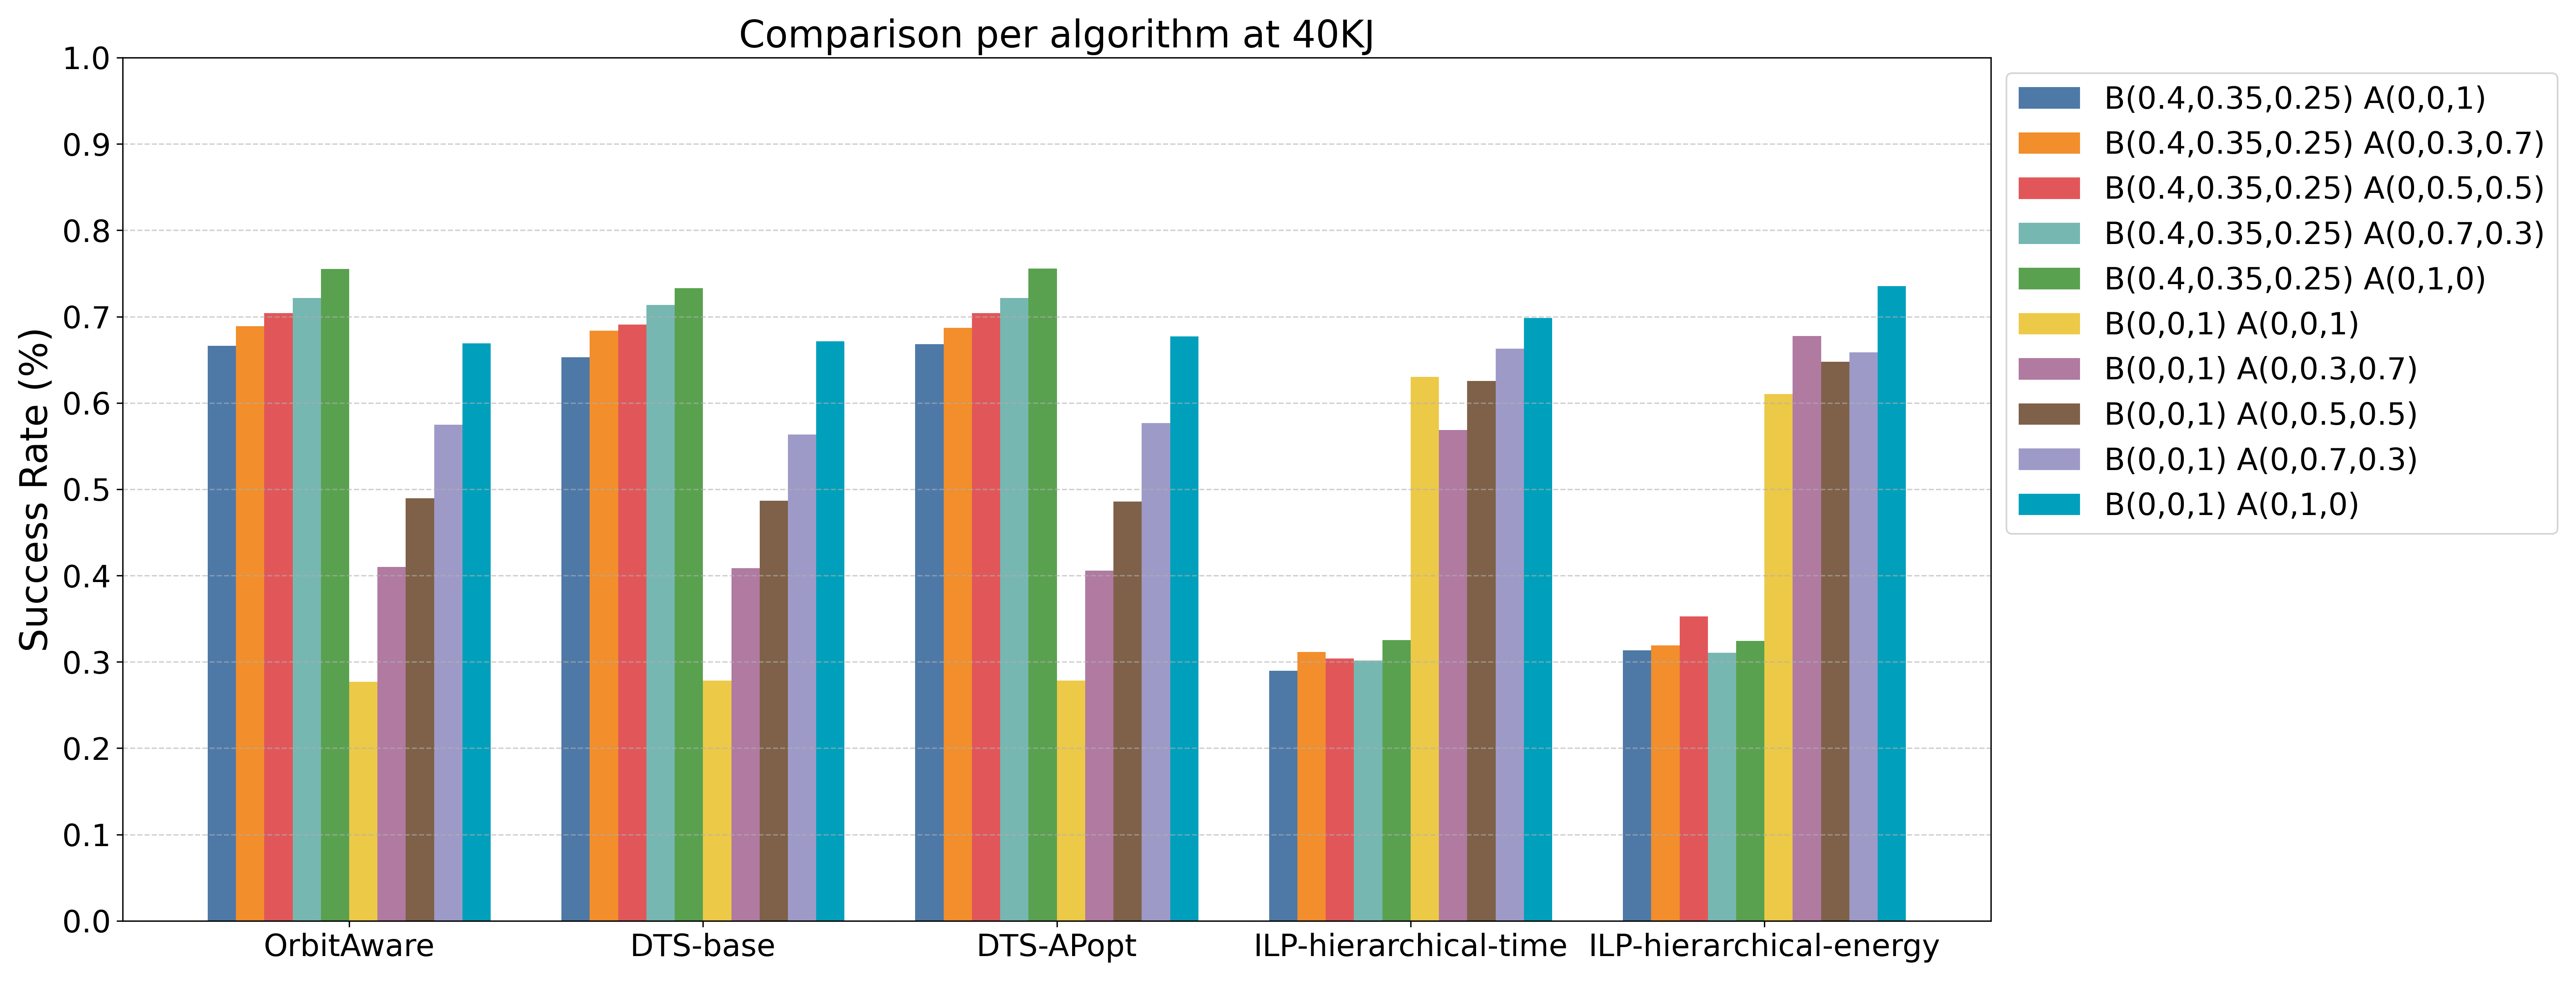
\includegraphics[width=0.9\paperwidth, height=0.4\textheight, keepaspectratio]{comparison_algos_40000.png} 
    \caption{Confronto algoritmi a 40KJ}
    \label{fig:grafico1}

    \vspace{1cm} % Spazio verticale tra i due grafici (regolalo a piacere)

    % --- SECONDO GRAFICO ---
    \noindent
    \hspace*{-3cm} 
    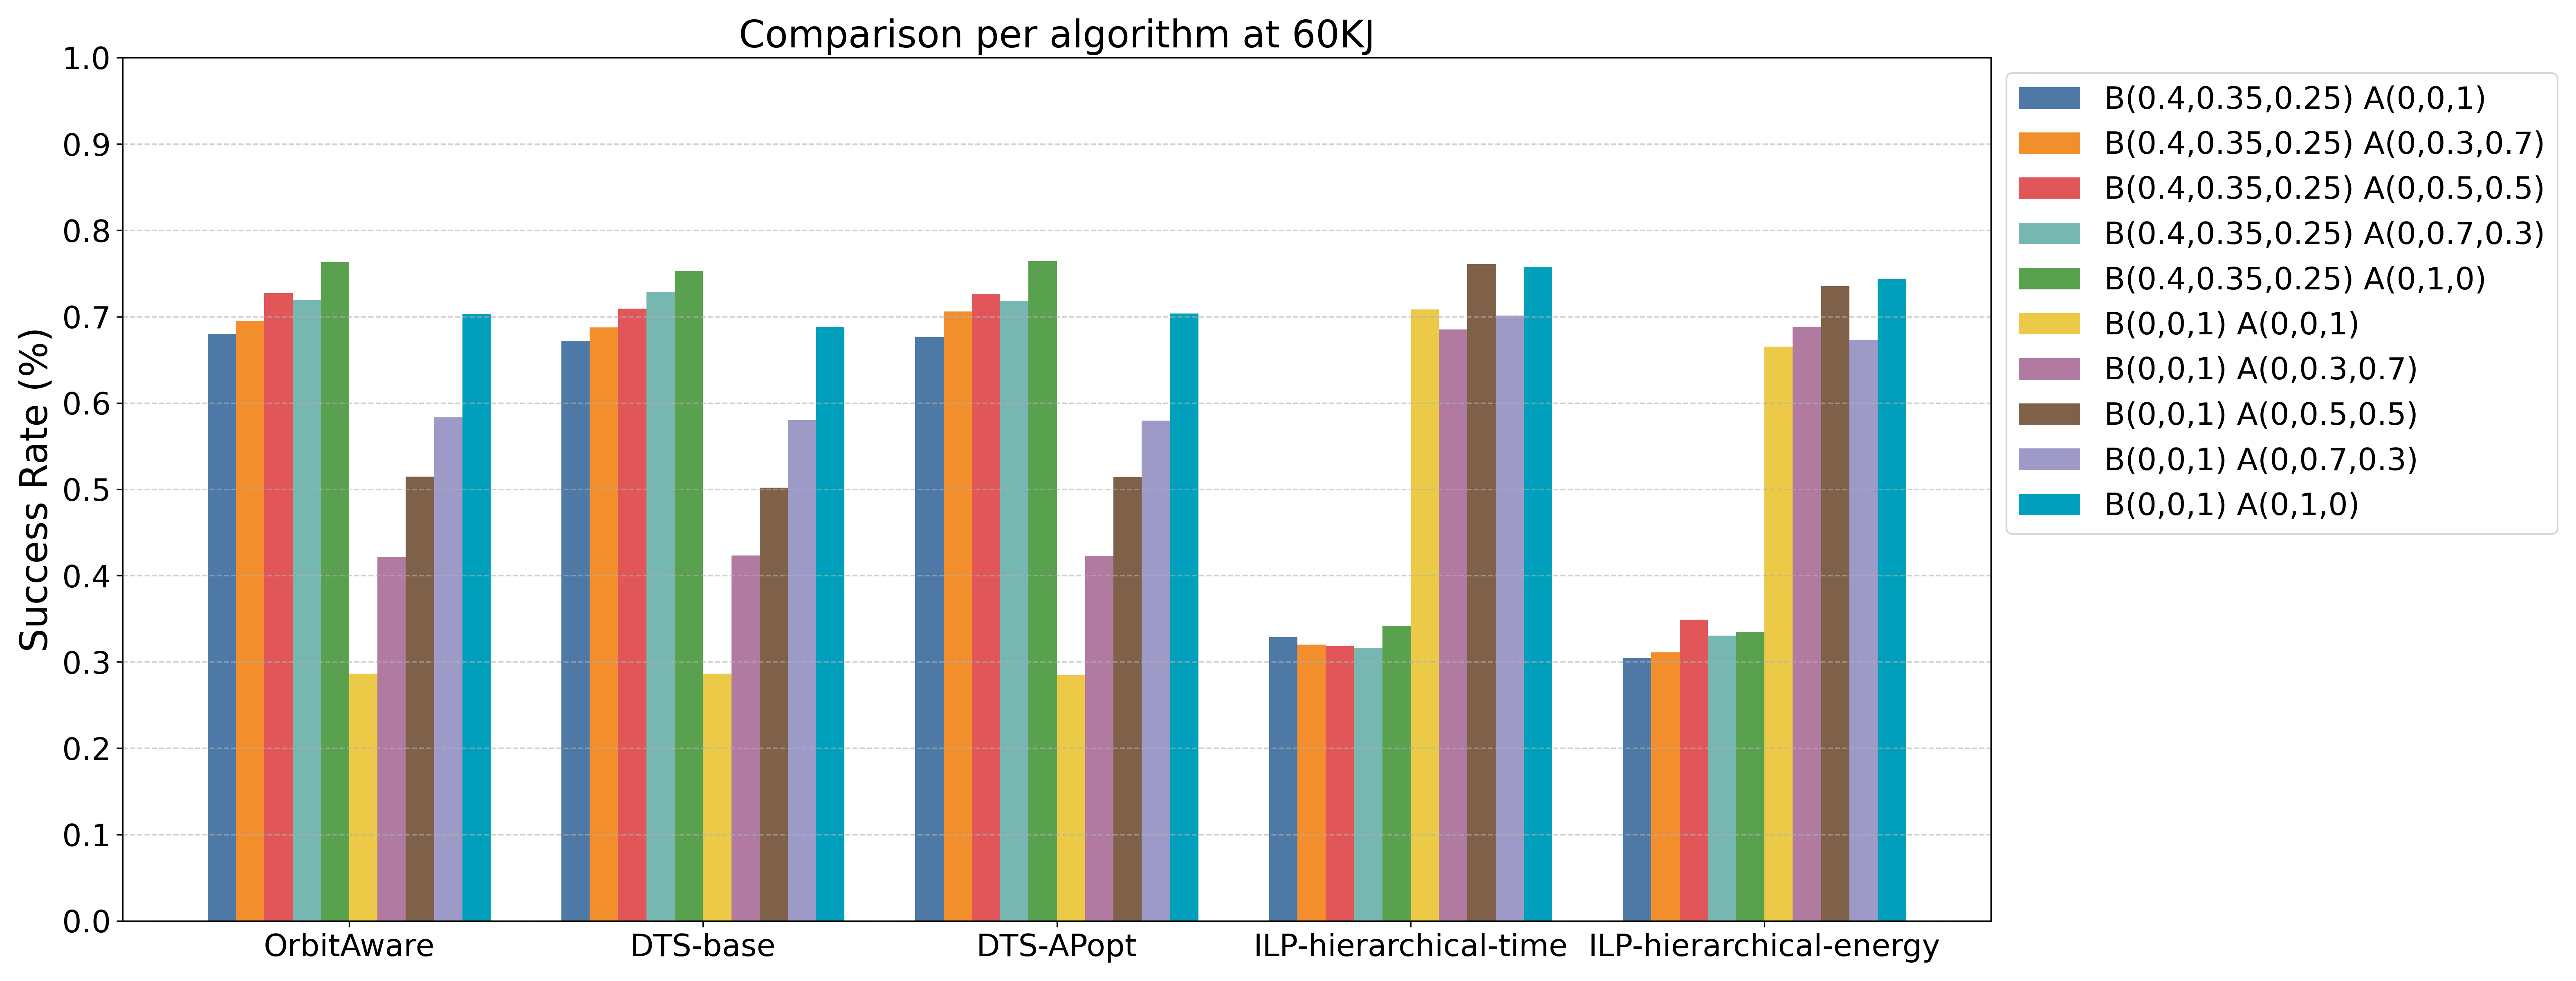
\includegraphics[width=0.9\paperwidth, height=0.4\textheight, keepaspectratio]{comparison_algos_60000.png} 
    \caption{Confronto algoritmi a 60KJ}
    \label{fig:grafico2}
\end{figure}

\begin{figure}[H] % Forza la posizione 'qui'
    \noindent 
    % --- PRIMO GRAFICO ---
    \hspace*{-3cm} 
    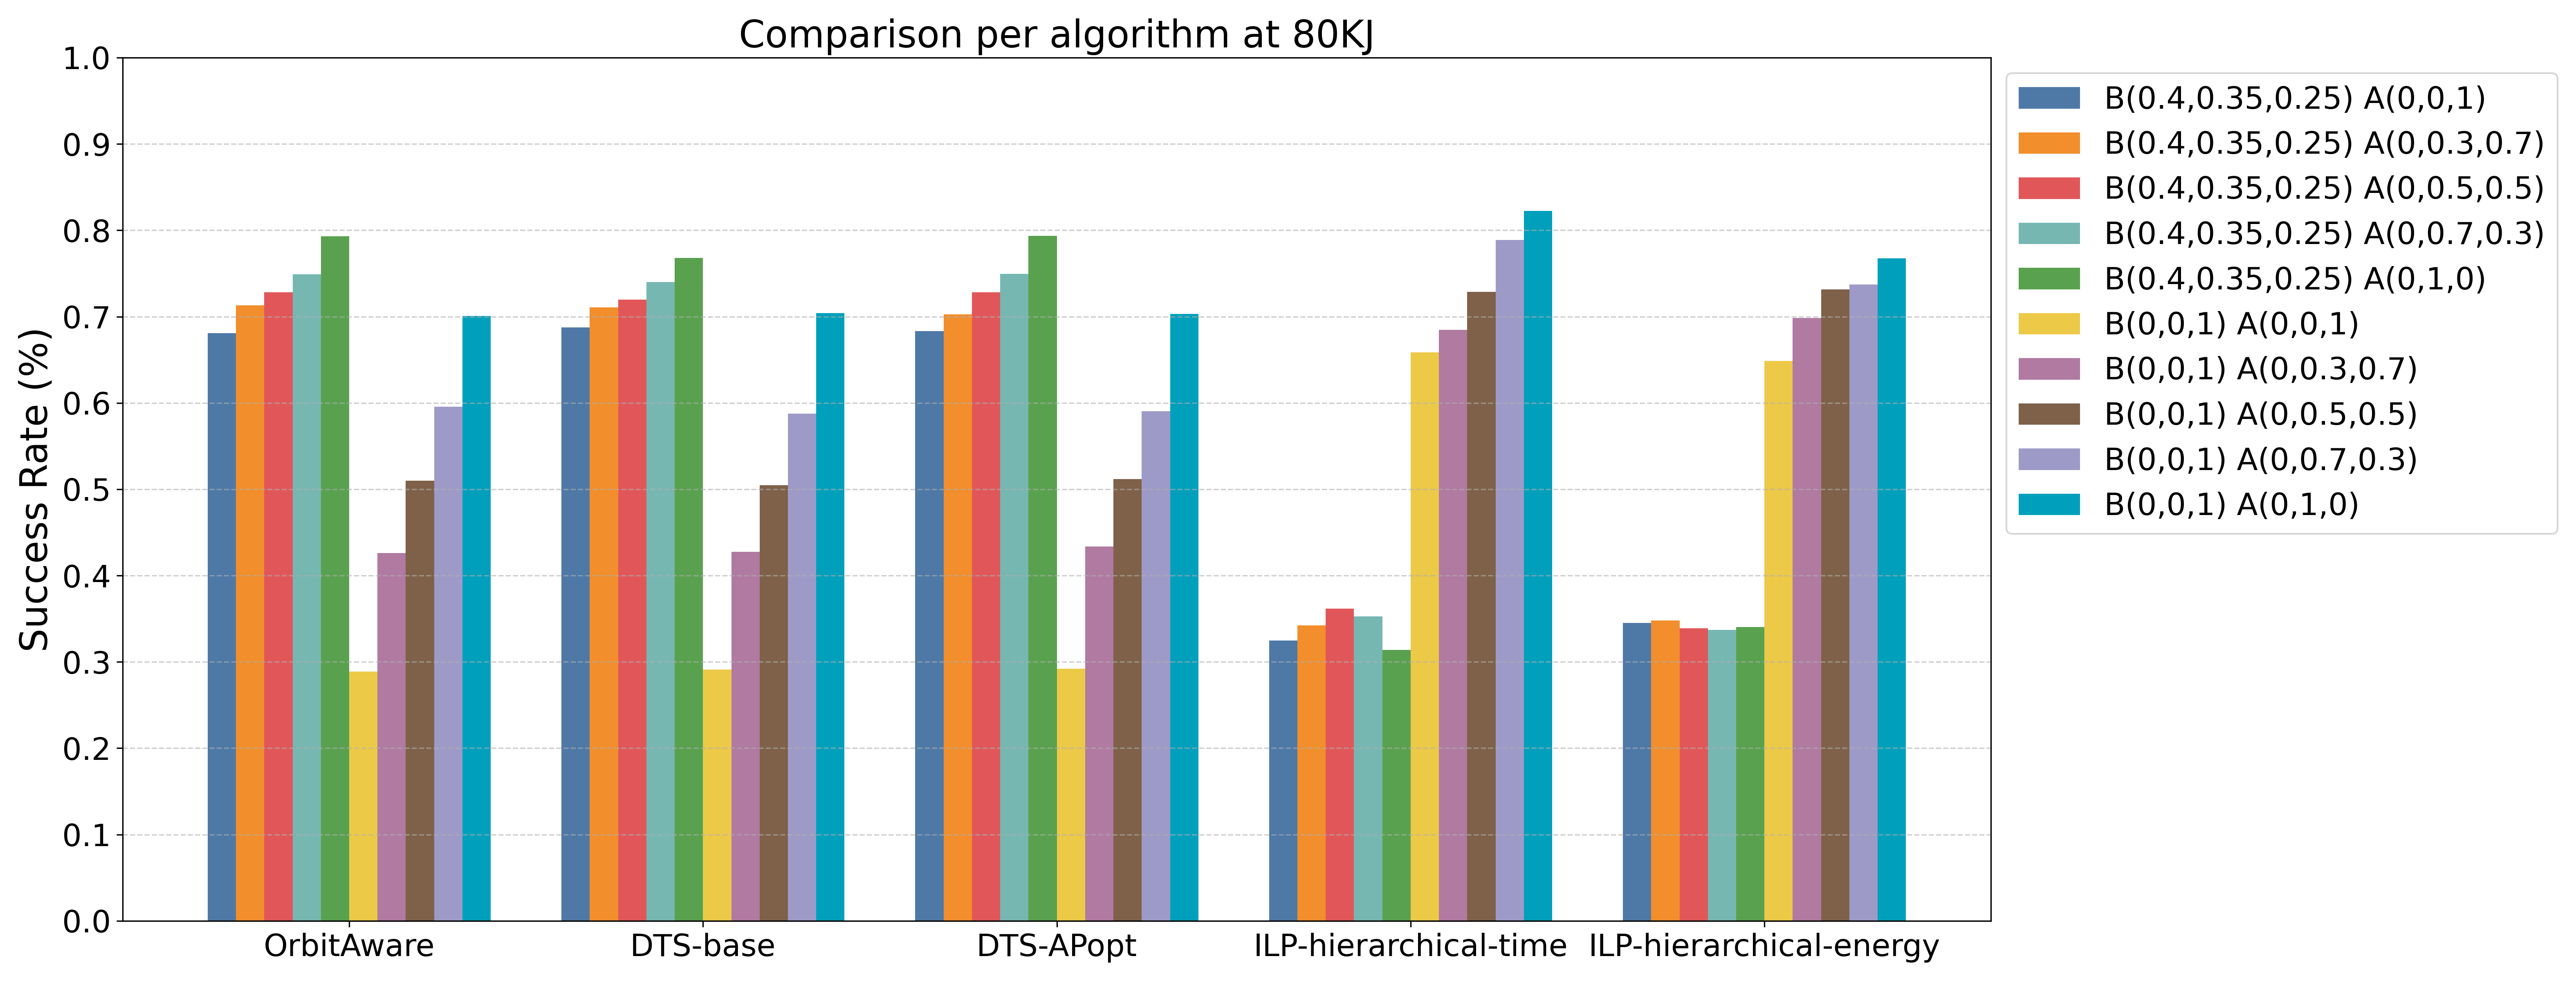
\includegraphics[width=0.9\paperwidth, height=0.4\textheight, keepaspectratio]{comparison_algos_80000.png} 
    \caption{Confronto algoritmi a 80KJ}
    \label{fig:grafico1}

    \vspace{1cm} % Spazio verticale tra i due grafici (regolalo a piacere)

    % --- SECONDO GRAFICO ---
    \noindent
    \hspace*{-3cm} 
    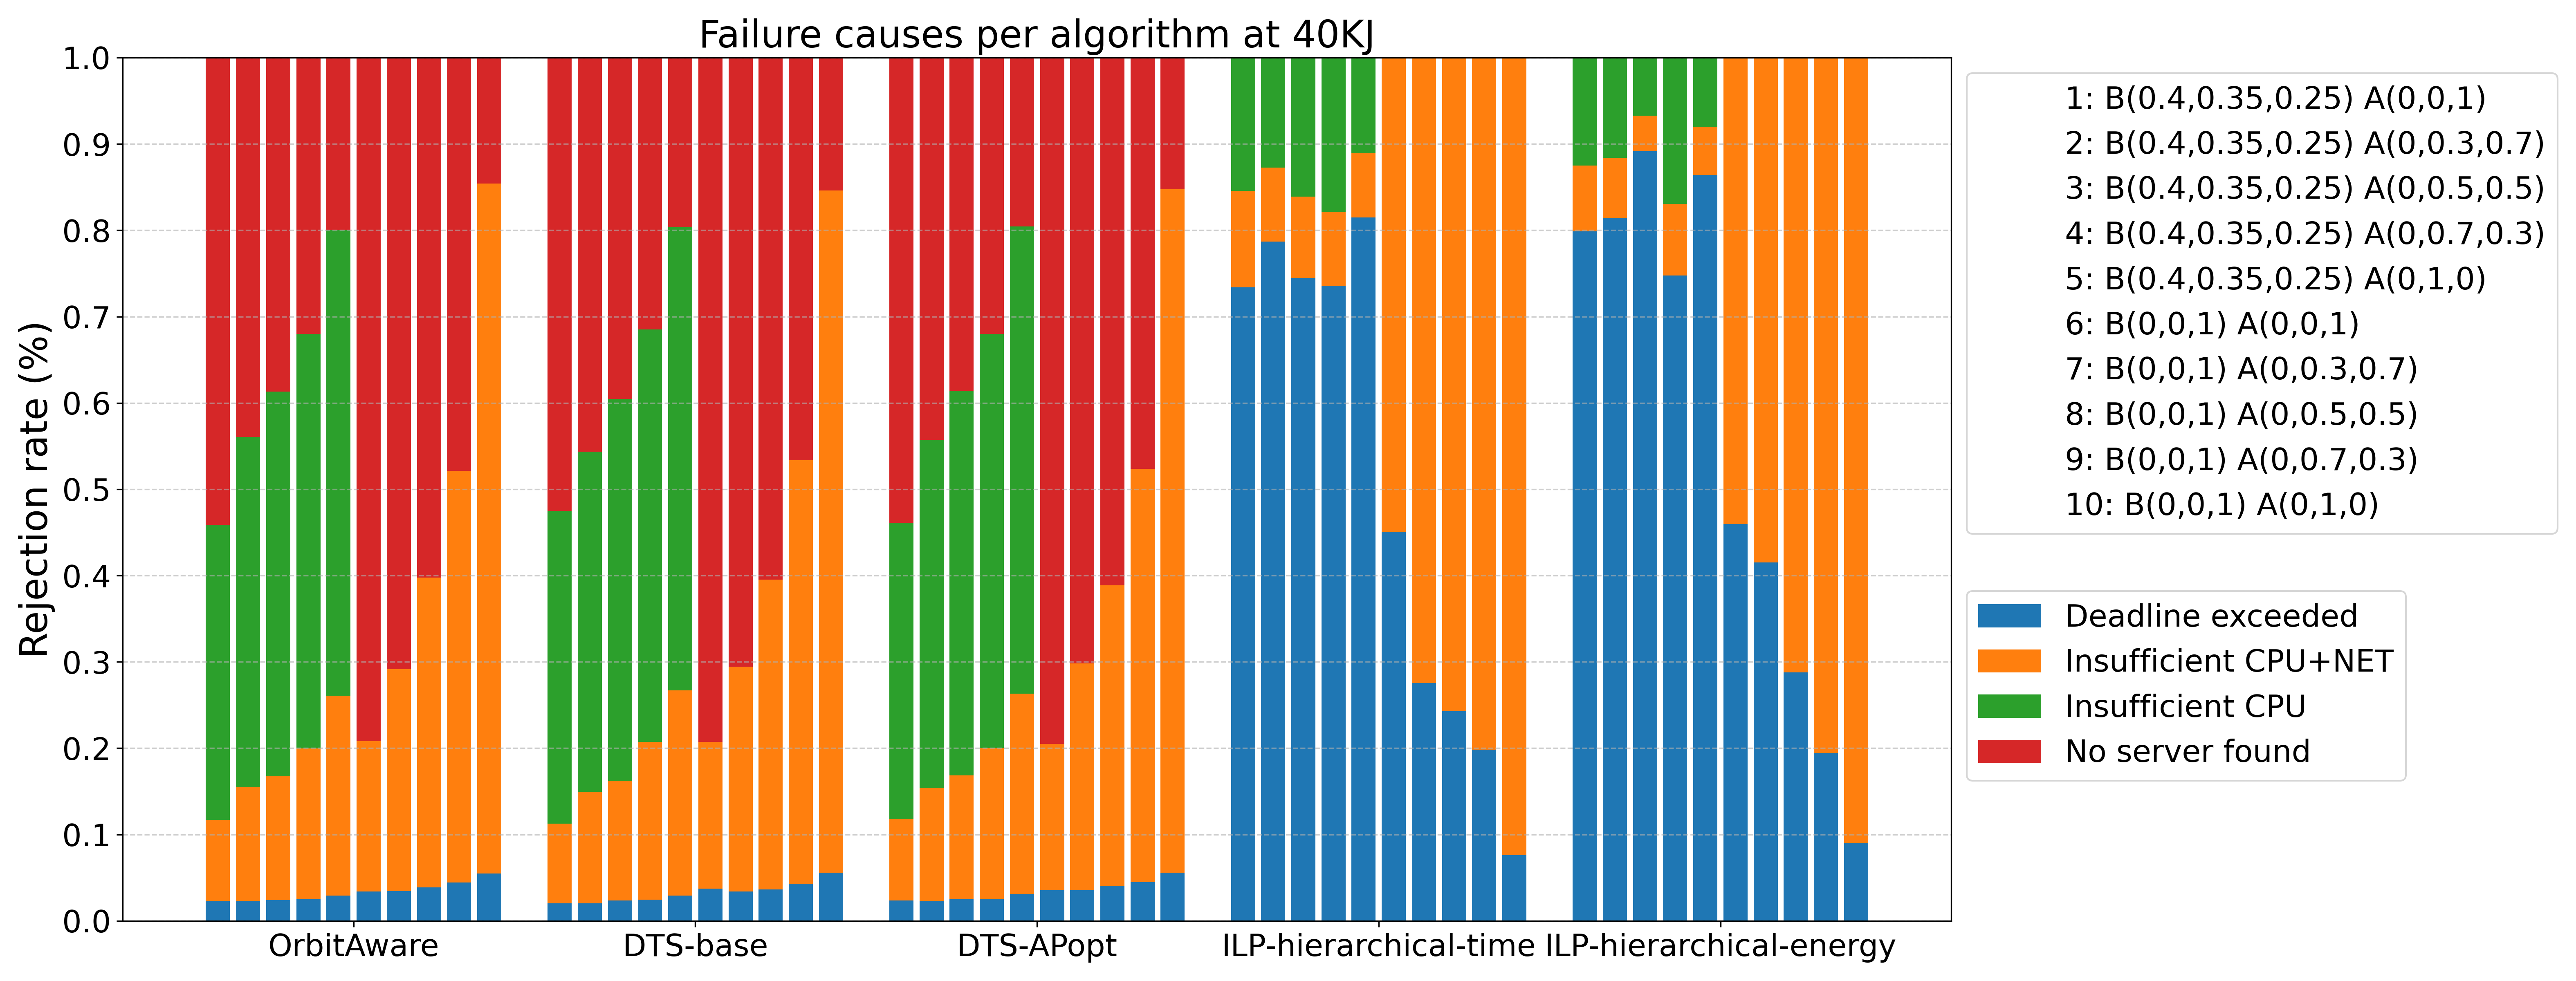
\includegraphics[width=0.9\paperwidth, height=0.4\textheight, keepaspectratio]{rejection_causes_40000.png} 
    \caption{Confronto rejection causes a 40KJ}
    \label{fig:grafico2}
\end{figure}

\begin{figure}[H] % Forza la posizione 'qui'
    \noindent 
    % --- PRIMO GRAFICO ---
    \hspace*{-3cm} 
    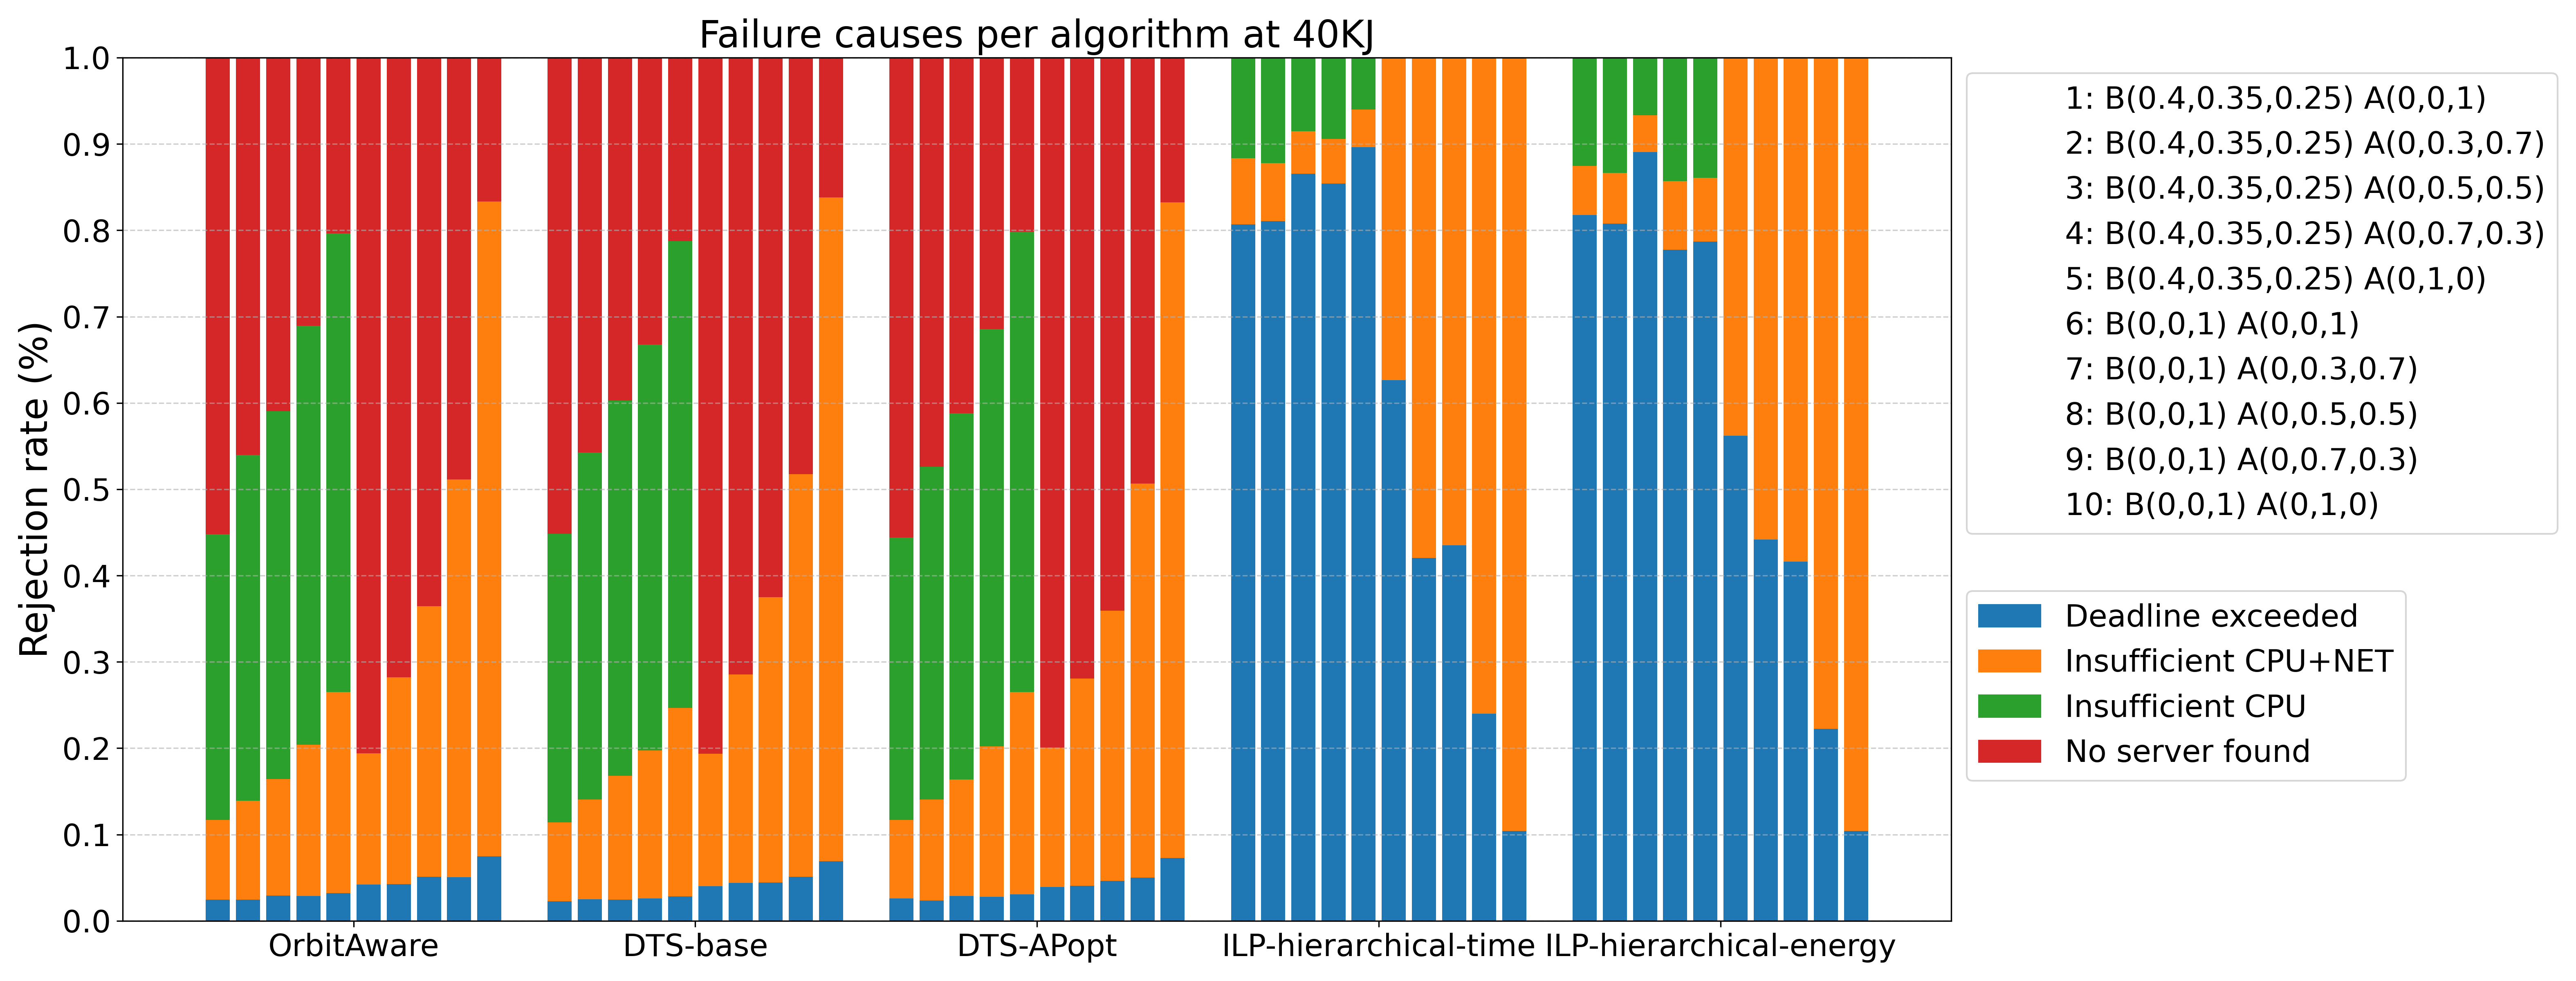
\includegraphics[width=0.9\paperwidth, height=0.4\textheight, keepaspectratio]{rejection_causes_60000.png} 
    \caption{Confronto rejection causes a 60KJ}
    \label{fig:grafico1}

    \vspace{1cm} % Spazio verticale tra i due grafici (regolalo a piacere)

    % --- SECONDO GRAFICO ---
    \noindent
    \hspace*{-3cm} 
    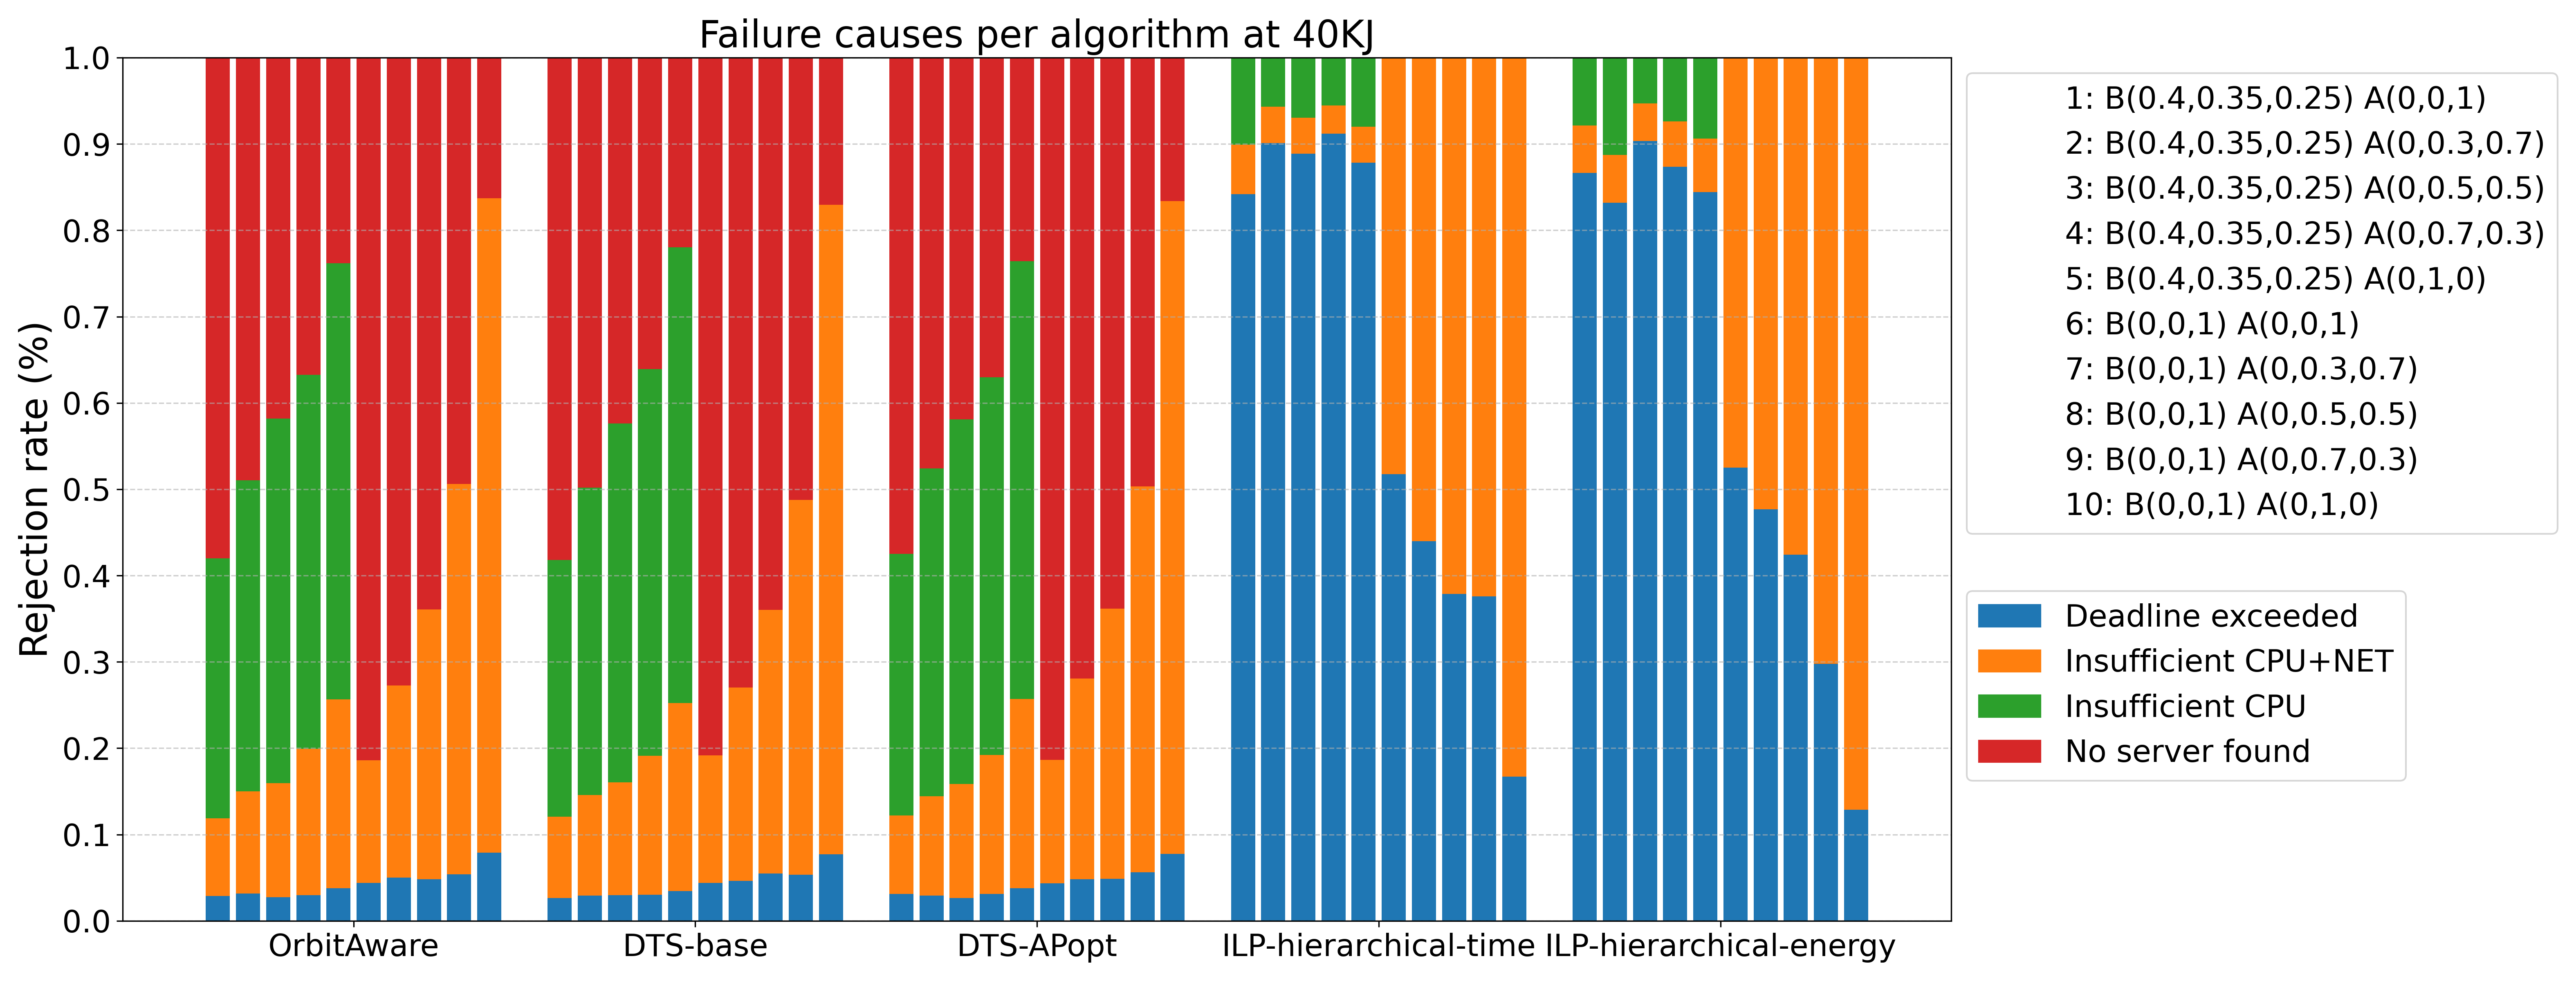
\includegraphics[width=0.9\paperwidth, height=0.4\textheight, keepaspectratio]{rejection_causes_80000.png} 
    \caption{Confronto rejection causes a 80KJ}
    \label{fig:grafico2}
\end{figure}

\begin{figure}[H] % Forza la posizione 'qui'
    \noindent 
    % --- PRIMO GRAFICO ---
    \hspace*{-3cm} 
    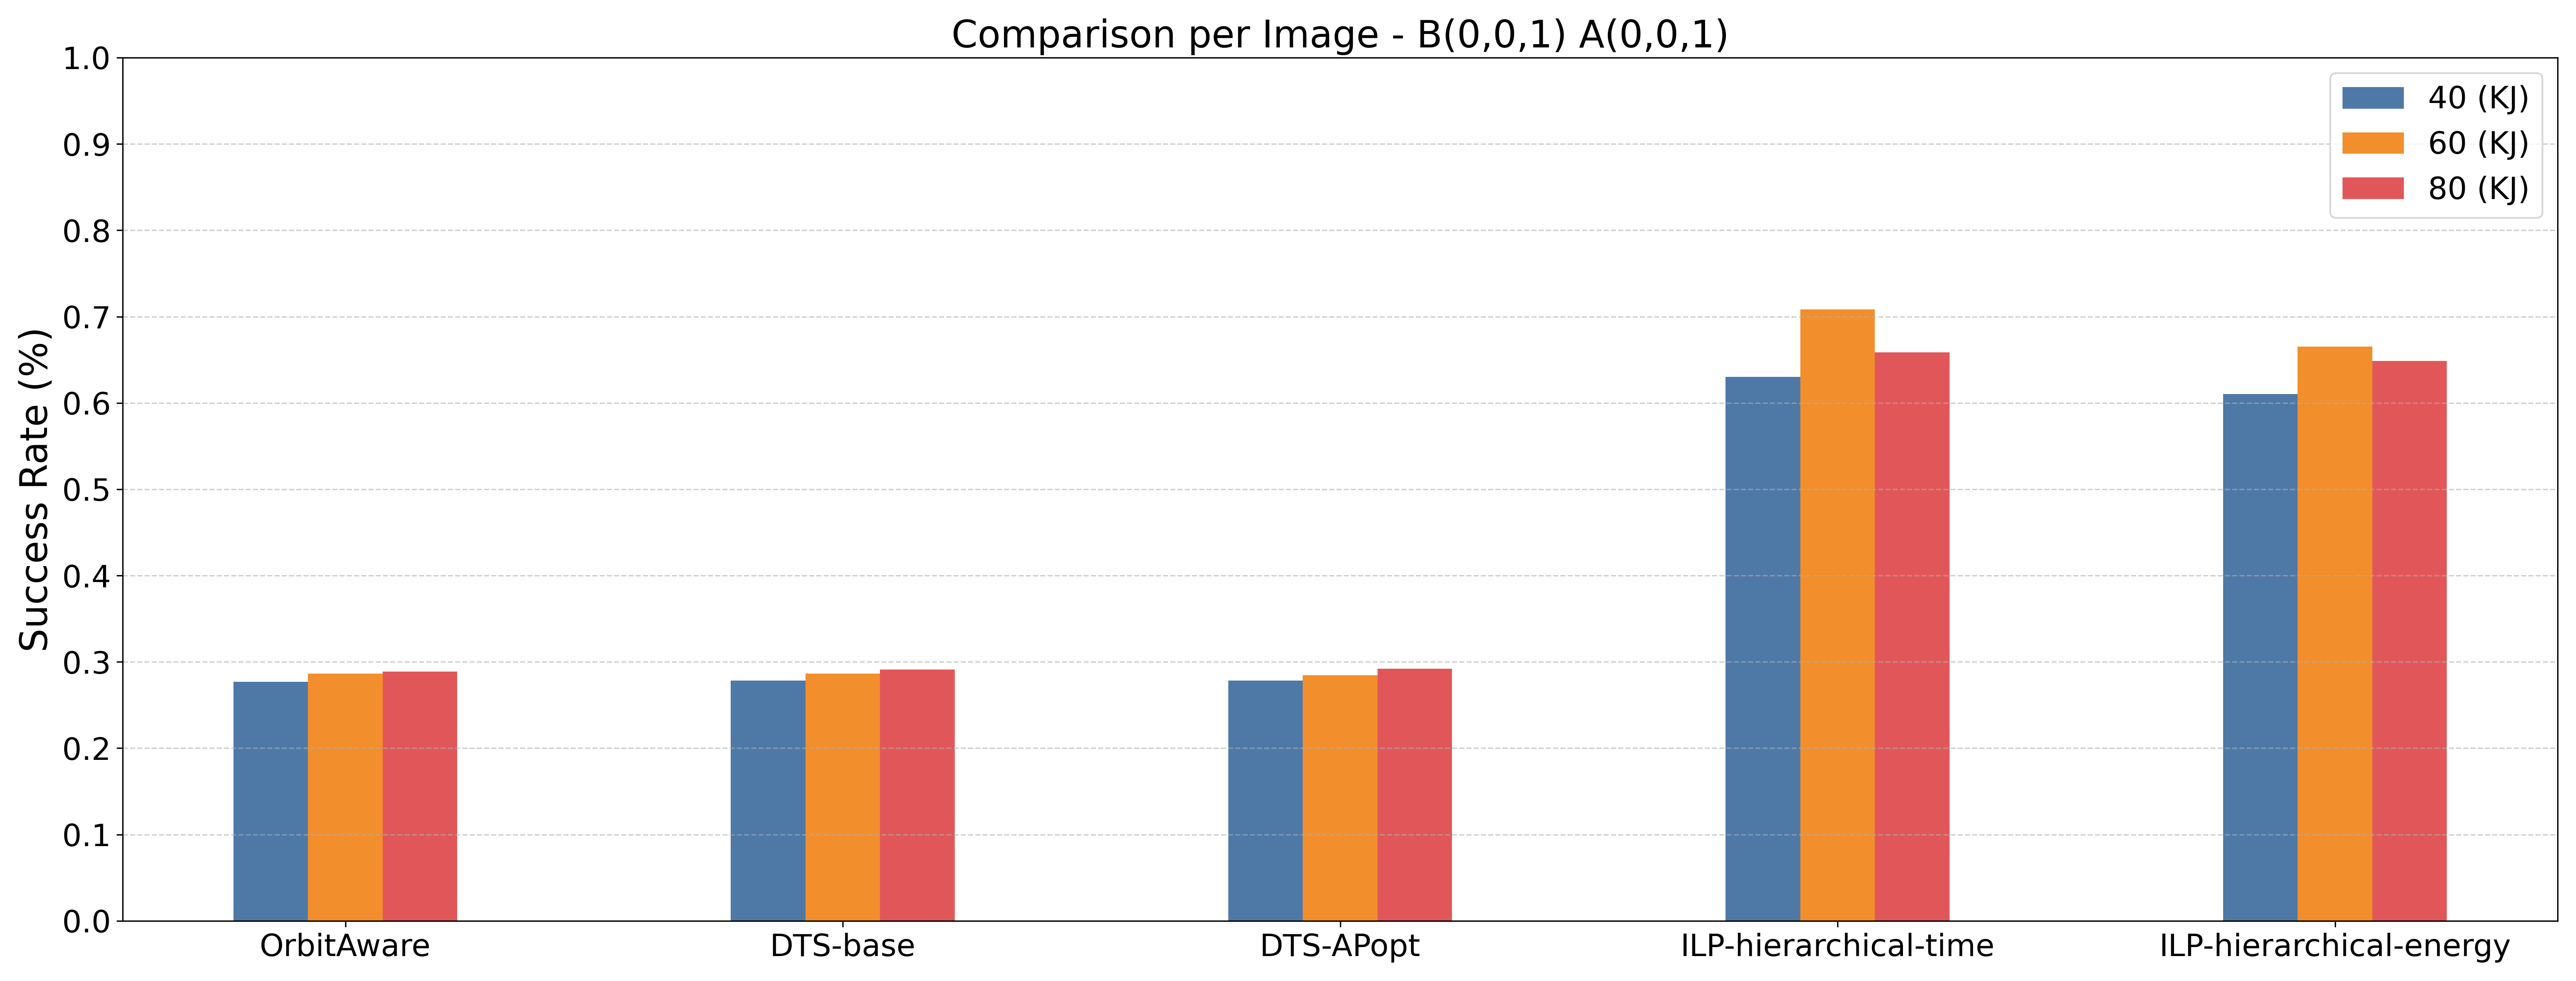
\includegraphics[width=0.9\paperwidth, height=0.4\textheight, keepaspectratio]{comparison_algos_img_0_0_1_0_0_1.png} 
    \caption{Confronto algoritmi con B(0,0,1) A(0,0,1)}
    \label{fig:grafico1}

    \vspace{1cm} % Spazio verticale tra i due grafici (regolalo a piacere)

    % --- SECONDO GRAFICO ---
    \noindent
    \hspace*{-3cm} 
    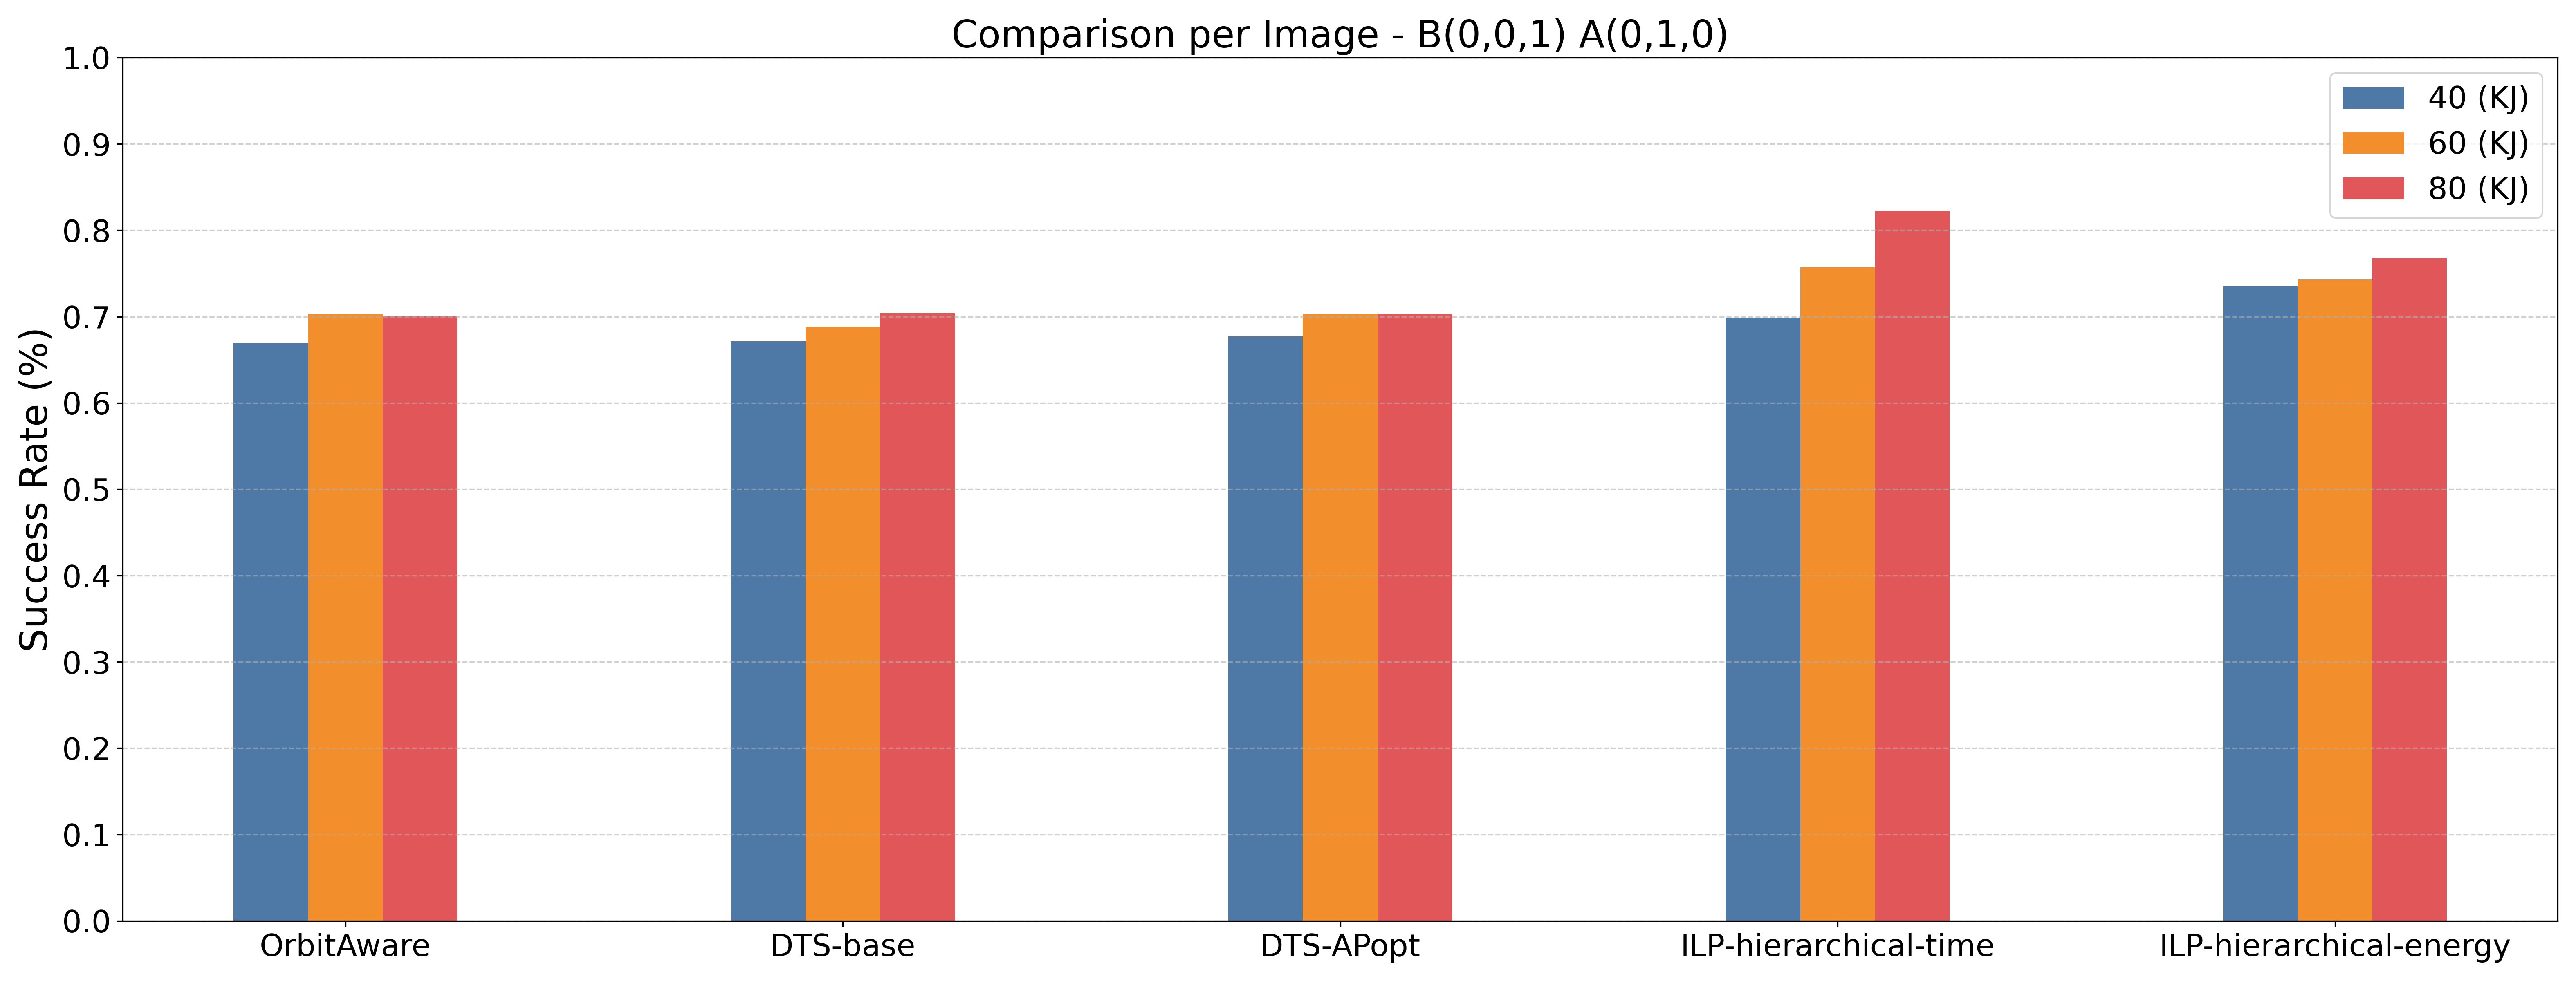
\includegraphics[width=0.9\paperwidth, height=0.4\textheight, keepaspectratio]{comparison_algos_img_0_0_1_0_1_0.png} 
    \caption{Confronto algoritmi con B(0,0,1) A(0,1,0)}
    \label{fig:grafico2}
\end{figure}

\begin{figure}[H] % Forza la posizione 'qui'
    \noindent 
    % --- PRIMO GRAFICO ---
    \hspace*{-3cm} 
    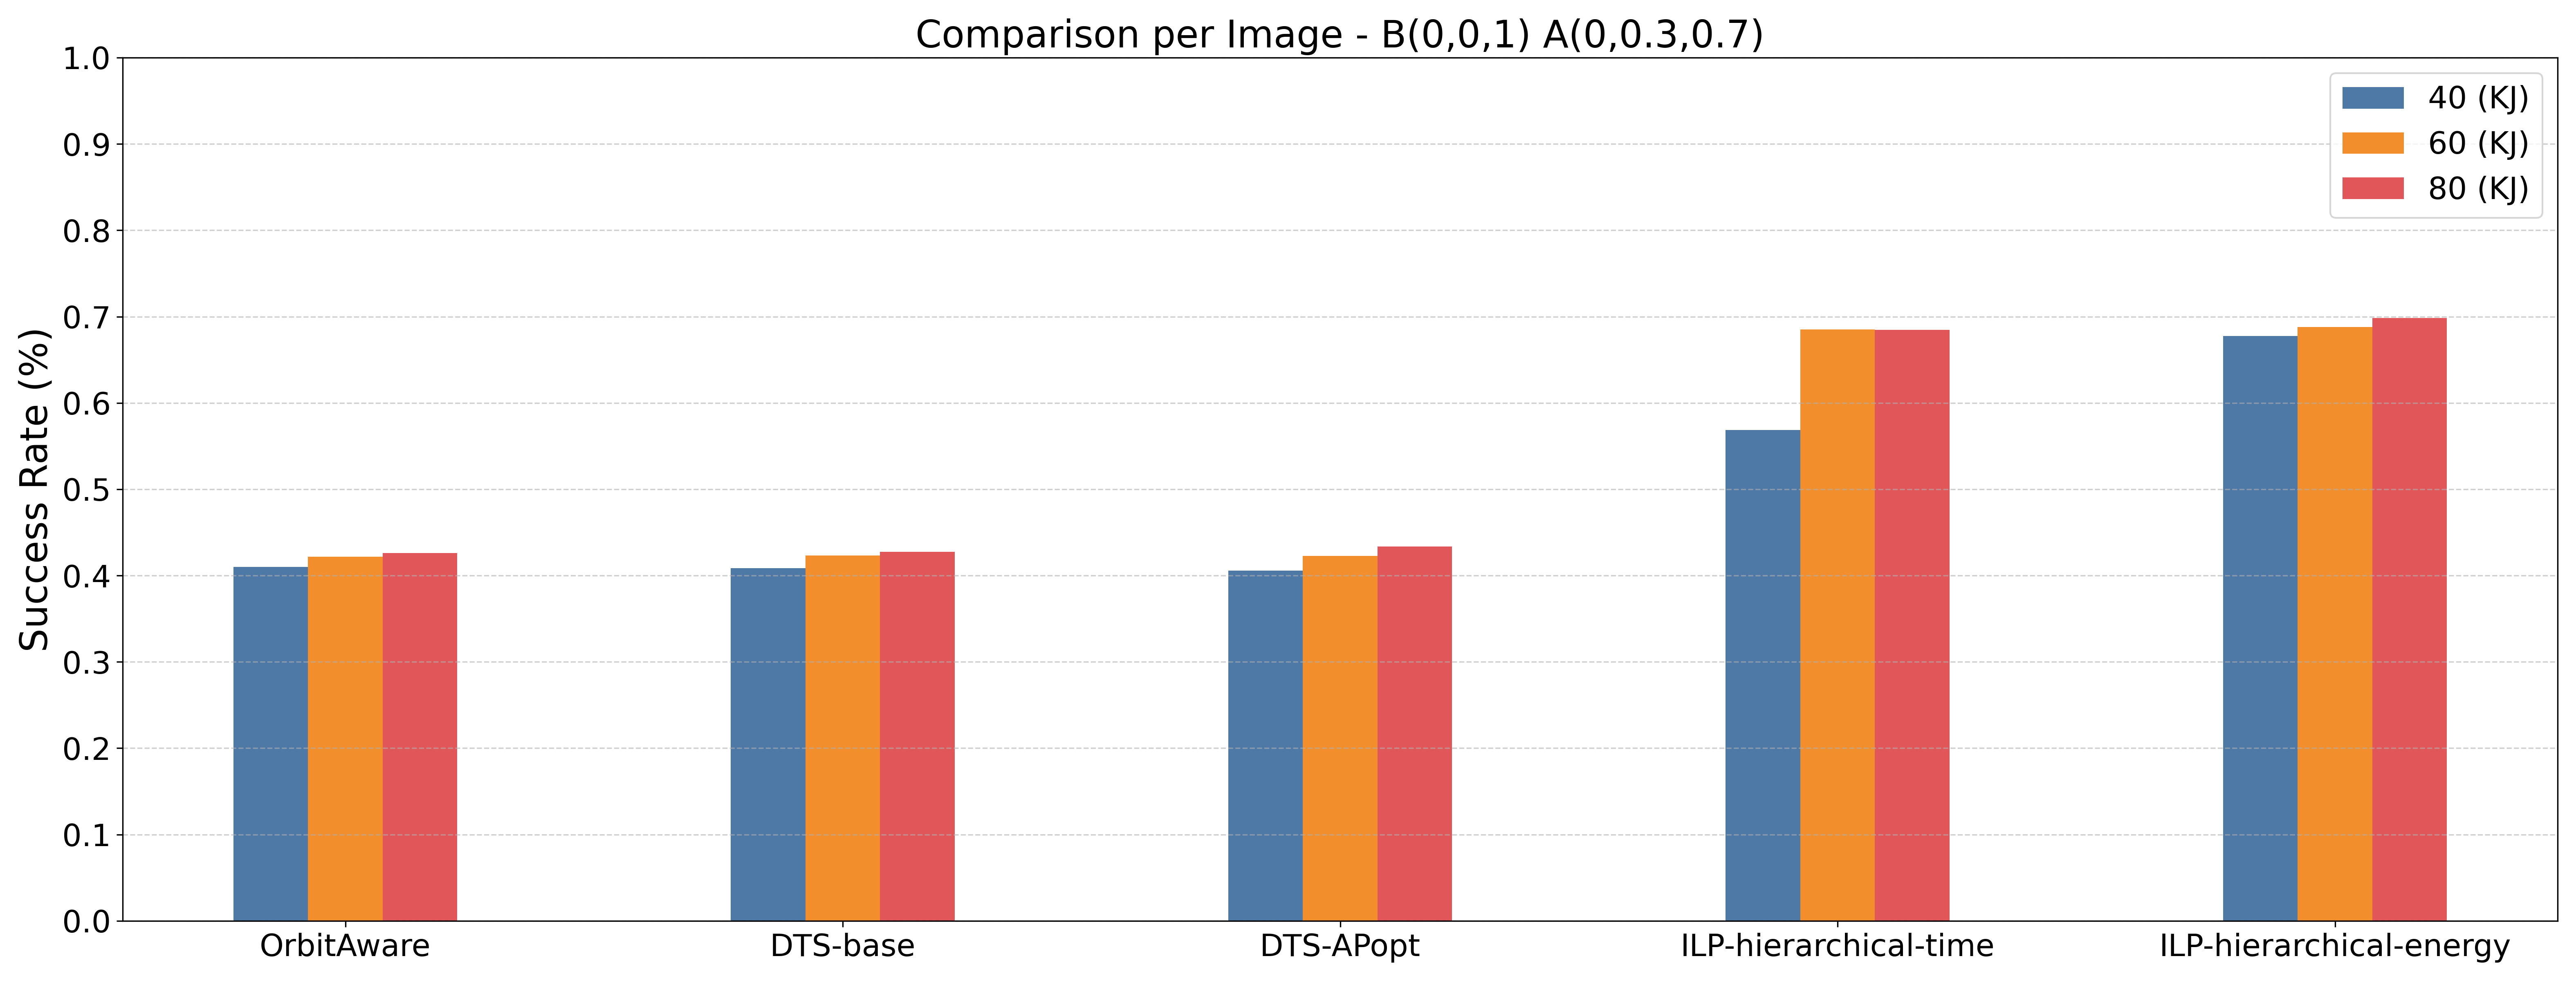
\includegraphics[width=0.9\paperwidth, height=0.4\textheight, keepaspectratio]{comparison_algos_img_0_0_1_0_0.3_0.7.png} 
    \caption{Confronto algoritmi con B(0,0,1) A(0,0.3,0.7)}
    \label{fig:grafico1}

    \vspace{1cm} % Spazio verticale tra i due grafici (regolalo a piacere)

    % --- SECONDO GRAFICO ---
    \noindent
    \hspace*{-3cm} 
    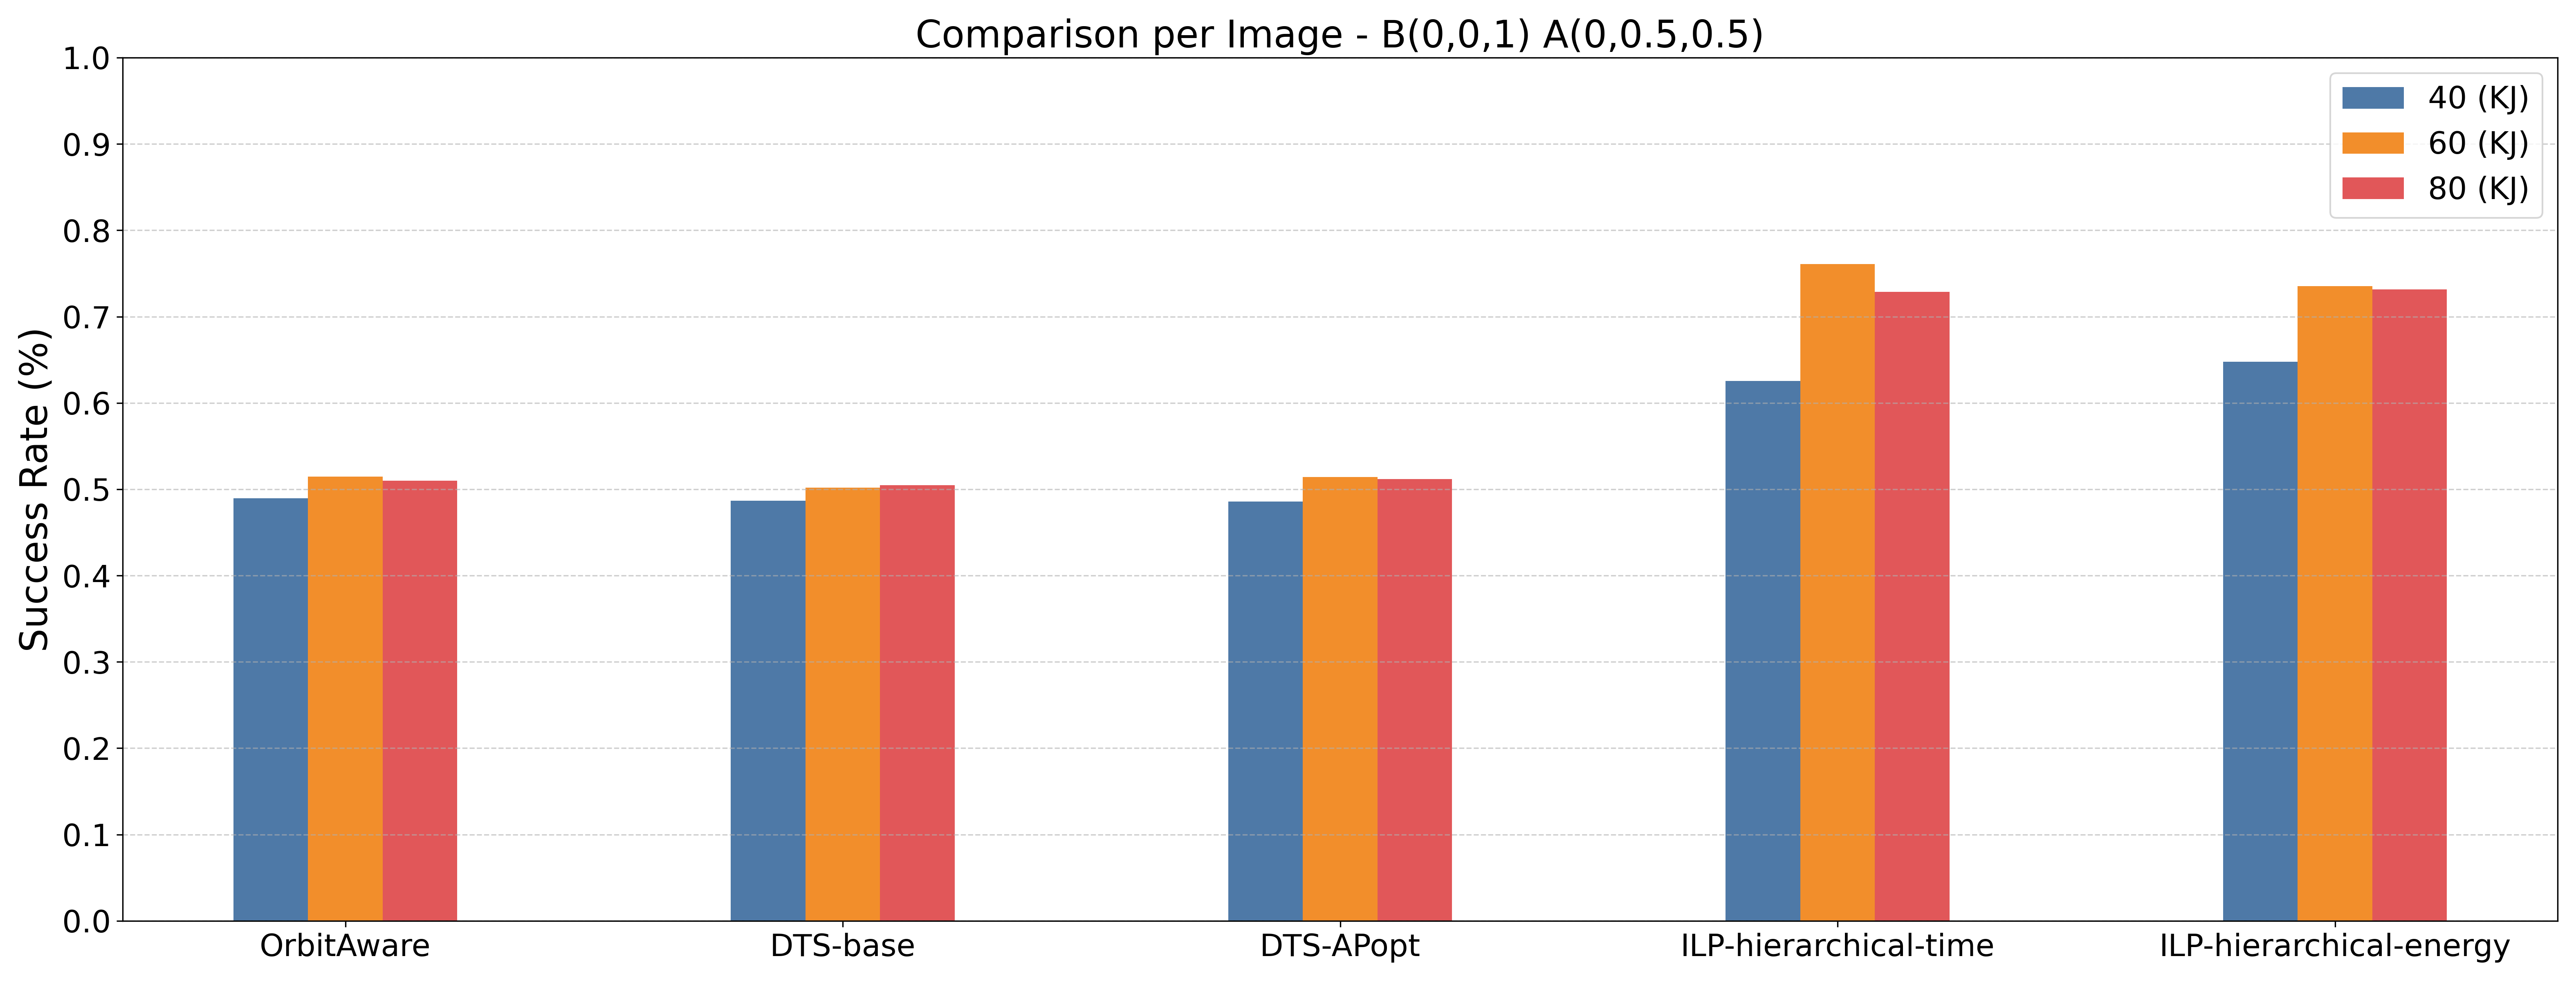
\includegraphics[width=0.9\paperwidth, height=0.4\textheight, keepaspectratio]{comparison_algos_img_0_0_1_0_0.5_0.5.png} 
    \caption{Confronto algoritmi con B(0,0,1) A(0,0.5,0.5)}
    \label{fig:grafico2}
\end{figure}

\begin{figure}[H] % Forza la posizione 'qui'
    \noindent 
    % --- PRIMO GRAFICO ---
    \hspace*{-3cm} 
    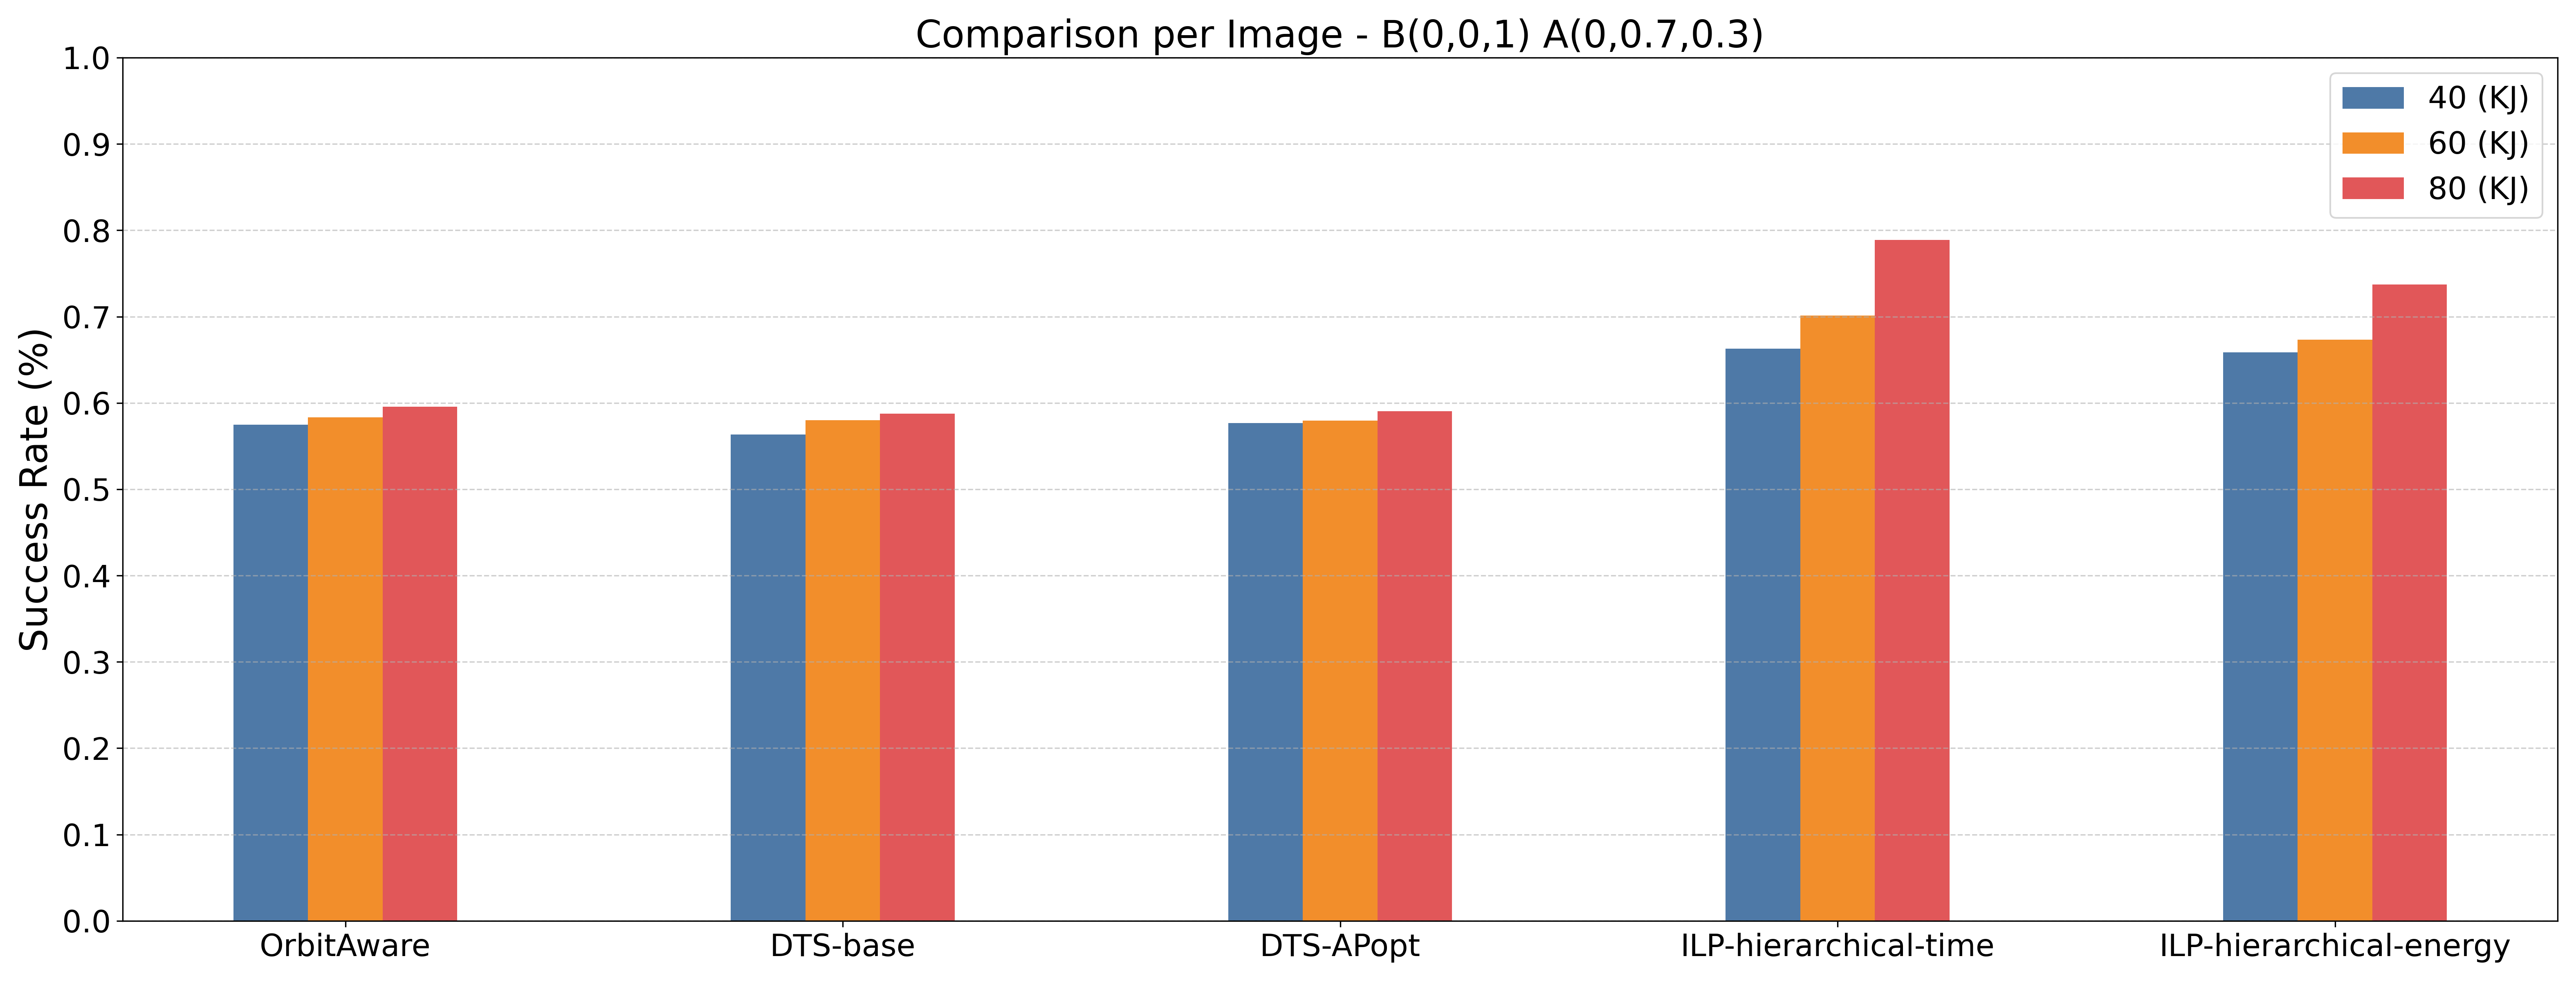
\includegraphics[width=0.9\paperwidth, height=0.4\textheight, keepaspectratio]{comparison_algos_img_0_0_1_0_0.7_0.3.png} 
    \caption{Confronto algoritmi con B(0,0,1) A(0,0.7,0.3)}
    \label{fig:grafico1}

    \vspace{1cm} % Spazio verticale tra i due grafici (regolalo a piacere)

    % --- SECONDO GRAFICO ---
    \noindent
    \hspace*{-3cm} 
    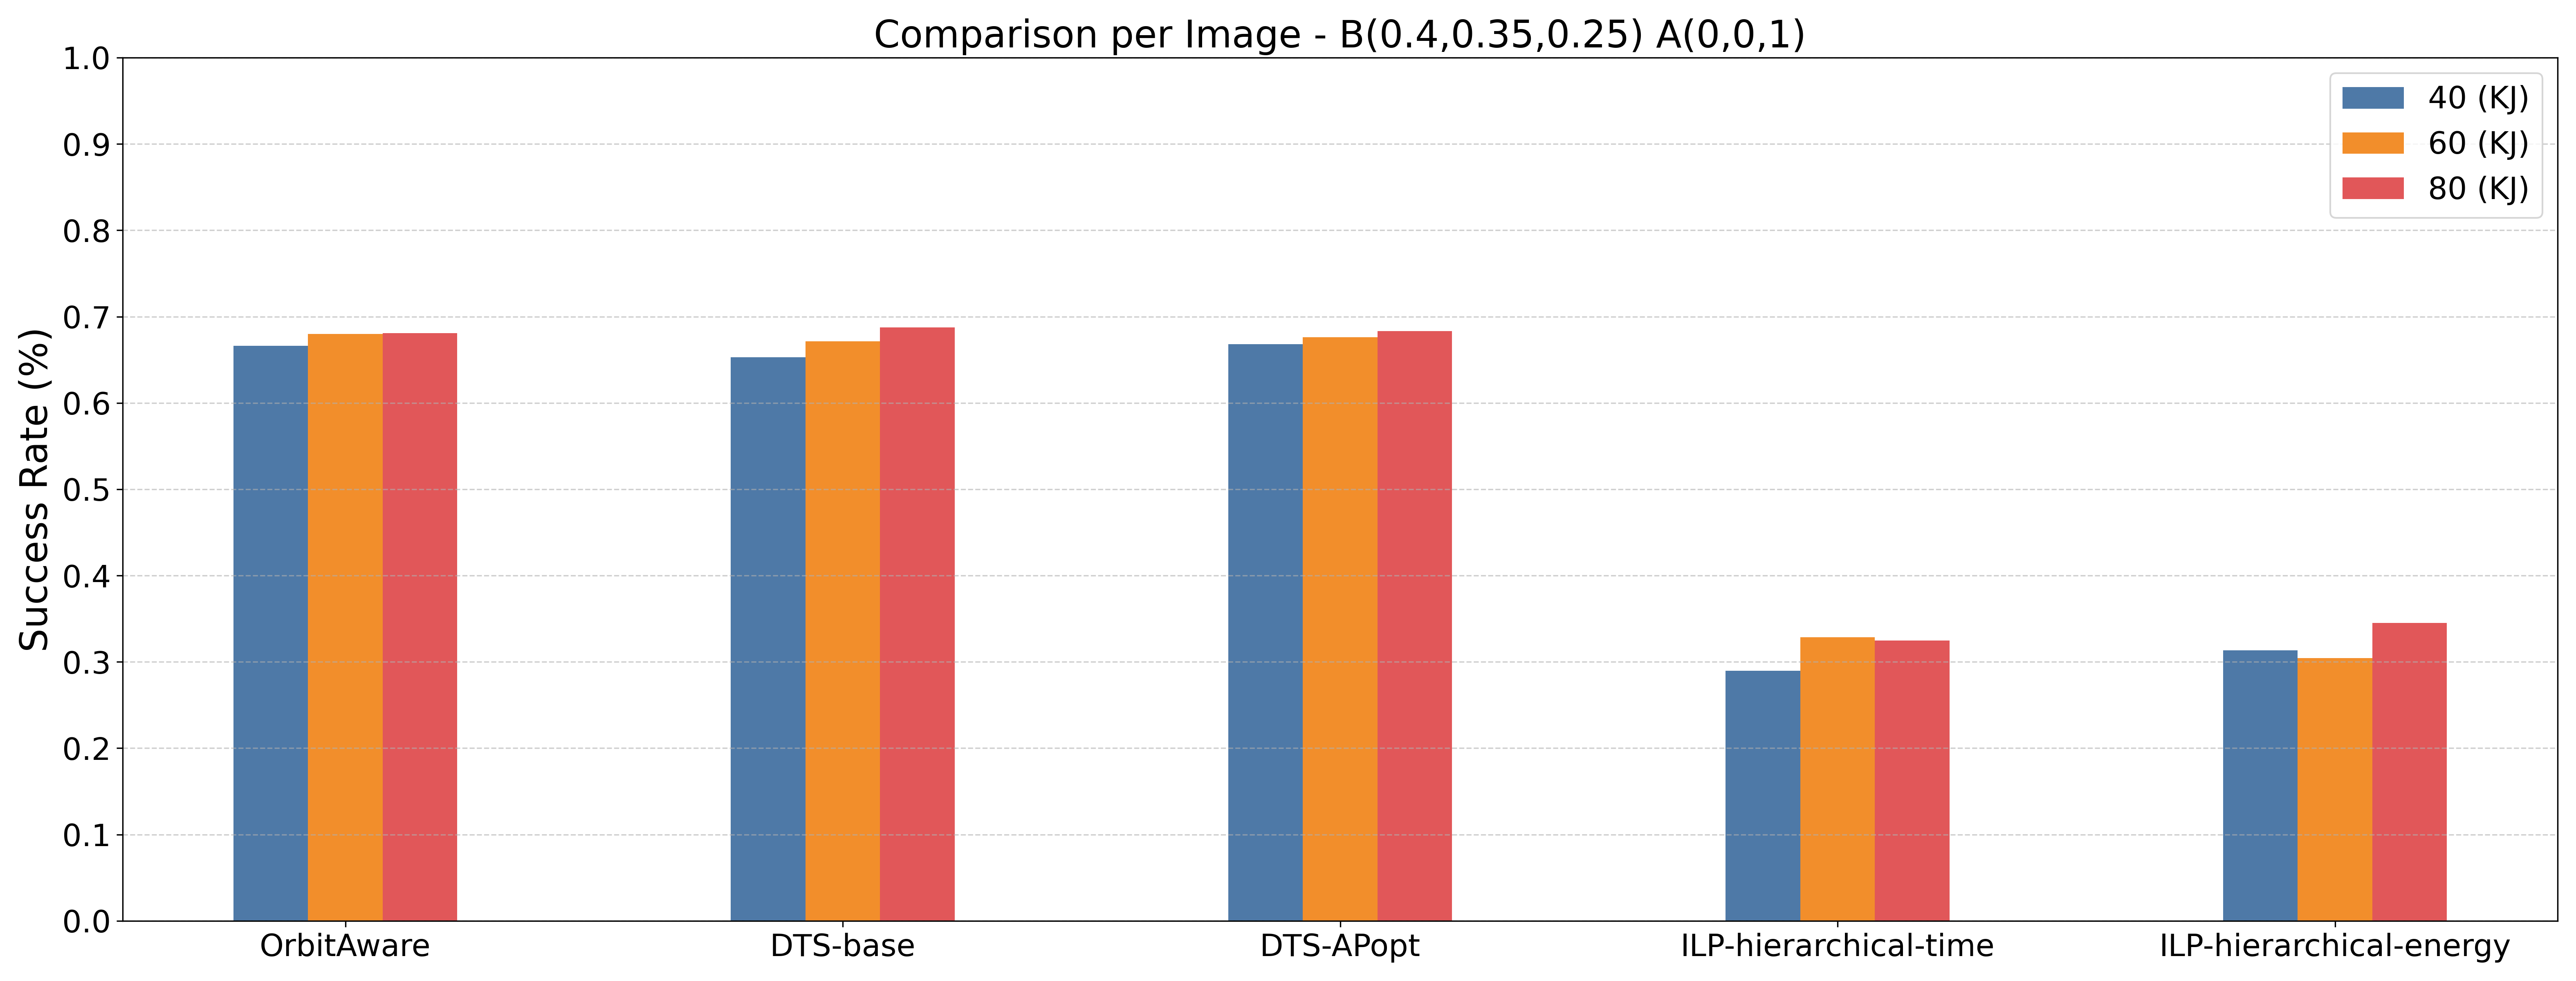
\includegraphics[width=0.9\paperwidth, height=0.4\textheight, keepaspectratio]{comparison_algos_img_0.45_0.35_0.25_0_0_1.png} 
    \caption{Confronto algoritmi con B(0.4,0.35,0.25) A(0,0,1)}
    \label{fig:grafico2}
\end{figure}

\begin{figure}[H] % Forza la posizione 'qui'
    \noindent 
    % --- PRIMO GRAFICO ---
    \hspace*{-3cm} 
    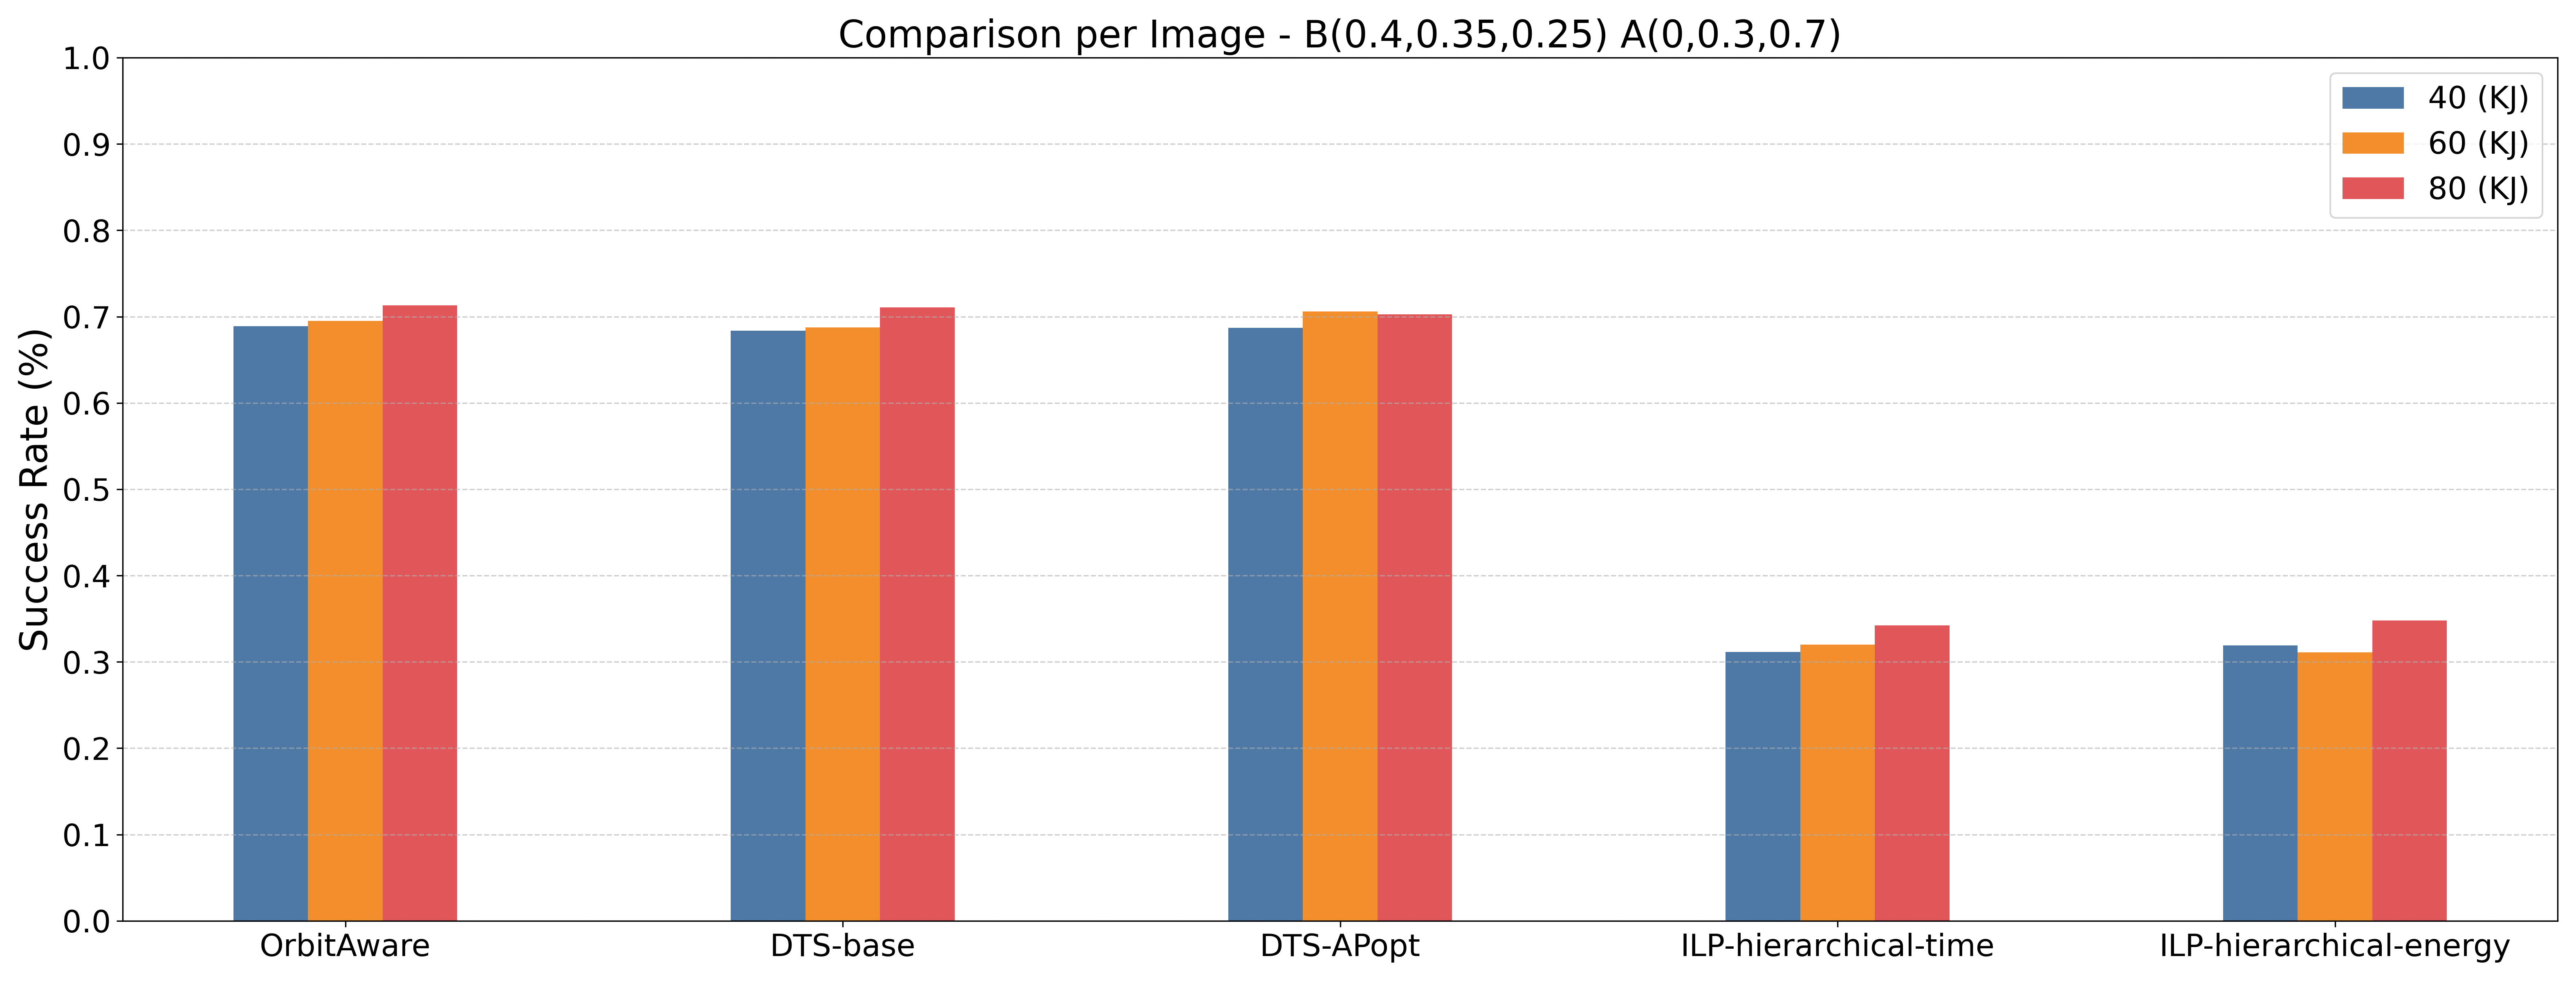
\includegraphics[width=0.9\paperwidth, height=0.4\textheight, keepaspectratio]{comparison_algos_img_0.45_0.35_0.25_0_0.3_0.7.png} 
    \caption{Confronto algoritmi con B(0.4,0.35,0.25) A(0,0.3,0.7)}
    \label{fig:grafico1}

    \vspace{1cm} % Spazio verticale tra i due grafici (regolalo a piacere)

    % --- SECONDO GRAFICO ---
    \noindent
    \hspace*{-3cm} 
    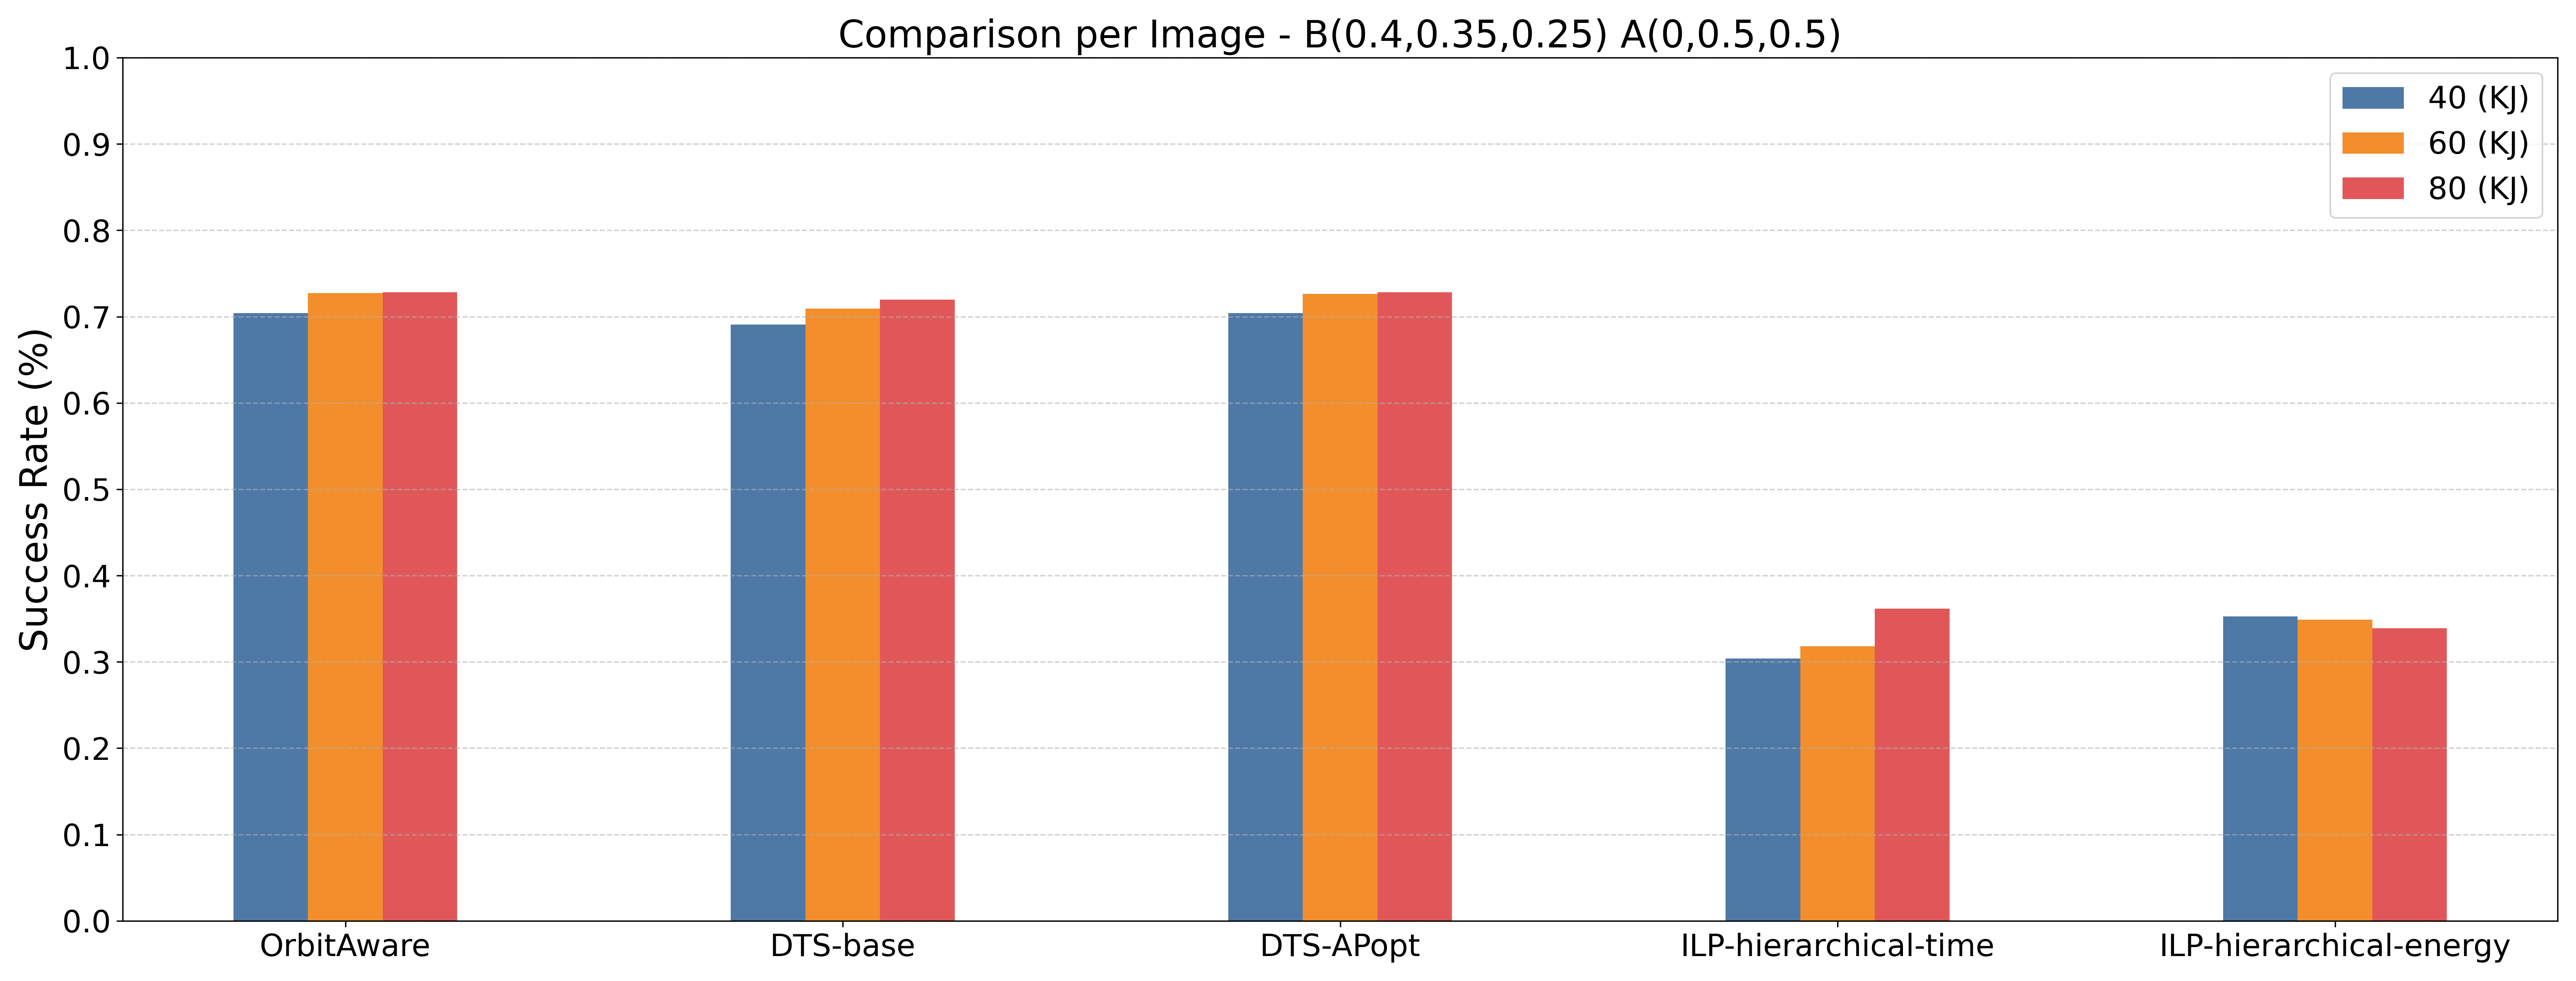
\includegraphics[width=0.9\paperwidth, height=0.4\textheight, keepaspectratio]{comparison_algos_img_0.45_0.35_0.25_0_0.5_0.5.png} 
    \caption{Confronto algoritmi con B(0.4,0.35,0.25) A(0,0.5,0.5)}
    \label{fig:grafico2}
\end{figure}

\begin{figure}[H] % Forza la posizione 'qui'
    \noindent 
    % --- PRIMO GRAFICO ---
    \hspace*{-3cm} 
    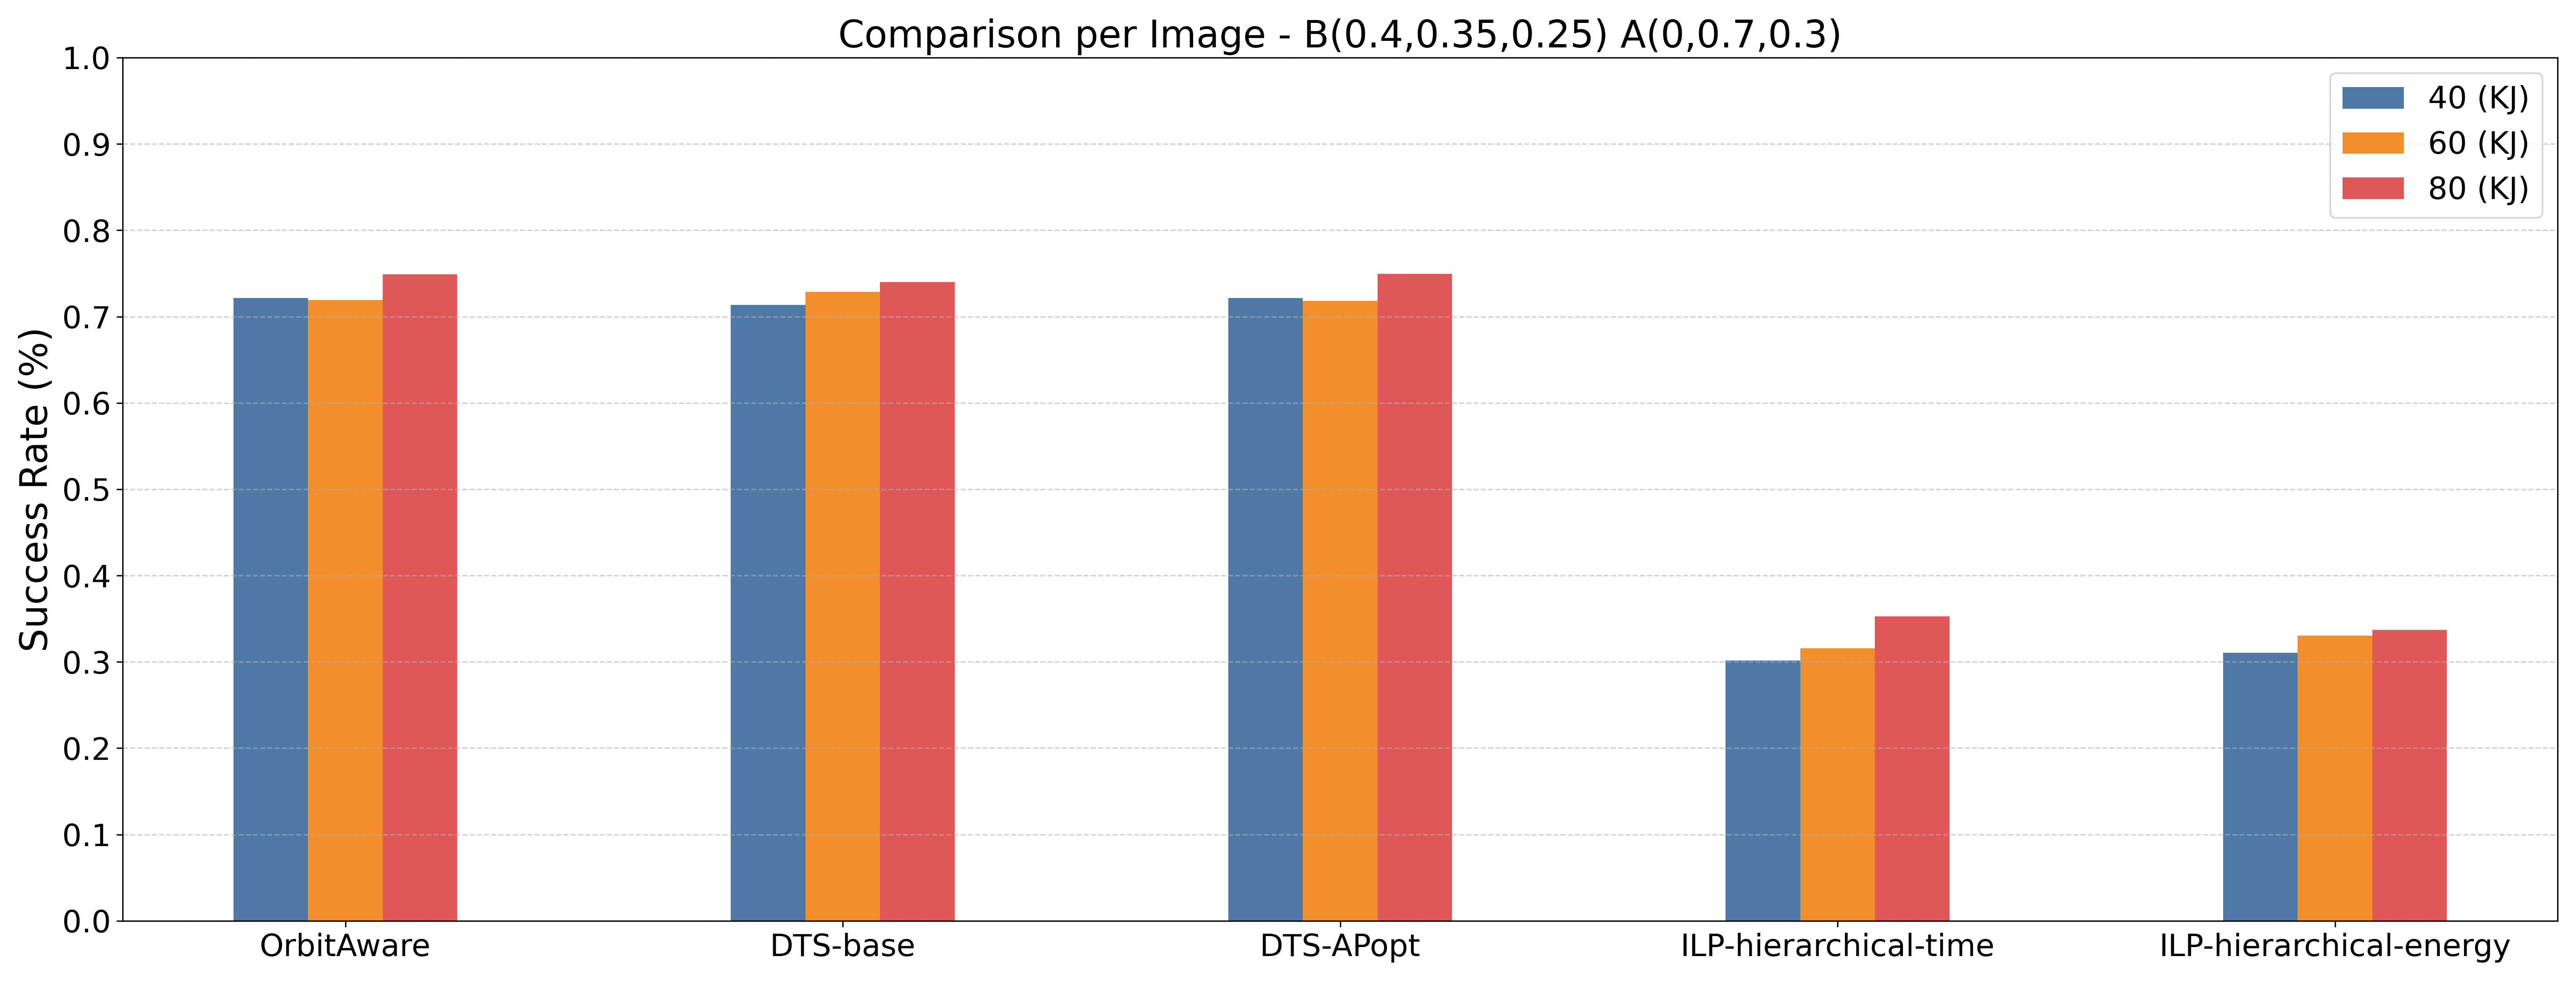
\includegraphics[width=0.9\paperwidth, height=0.4\textheight, keepaspectratio]{comparison_algos_img_0.45_0.35_0.25_0_0.7_0.3.png} 
    \caption{Confronto algoritmi con B(0.4,0.35,0.25) A(0,0.7,0.3)}
    \label{fig:grafico1}

    \vspace{1cm} % Spazio verticale tra i due grafici (regolalo a piacere)

    % --- SECONDO GRAFICO ---
    \noindent
    \hspace*{-3cm} 
    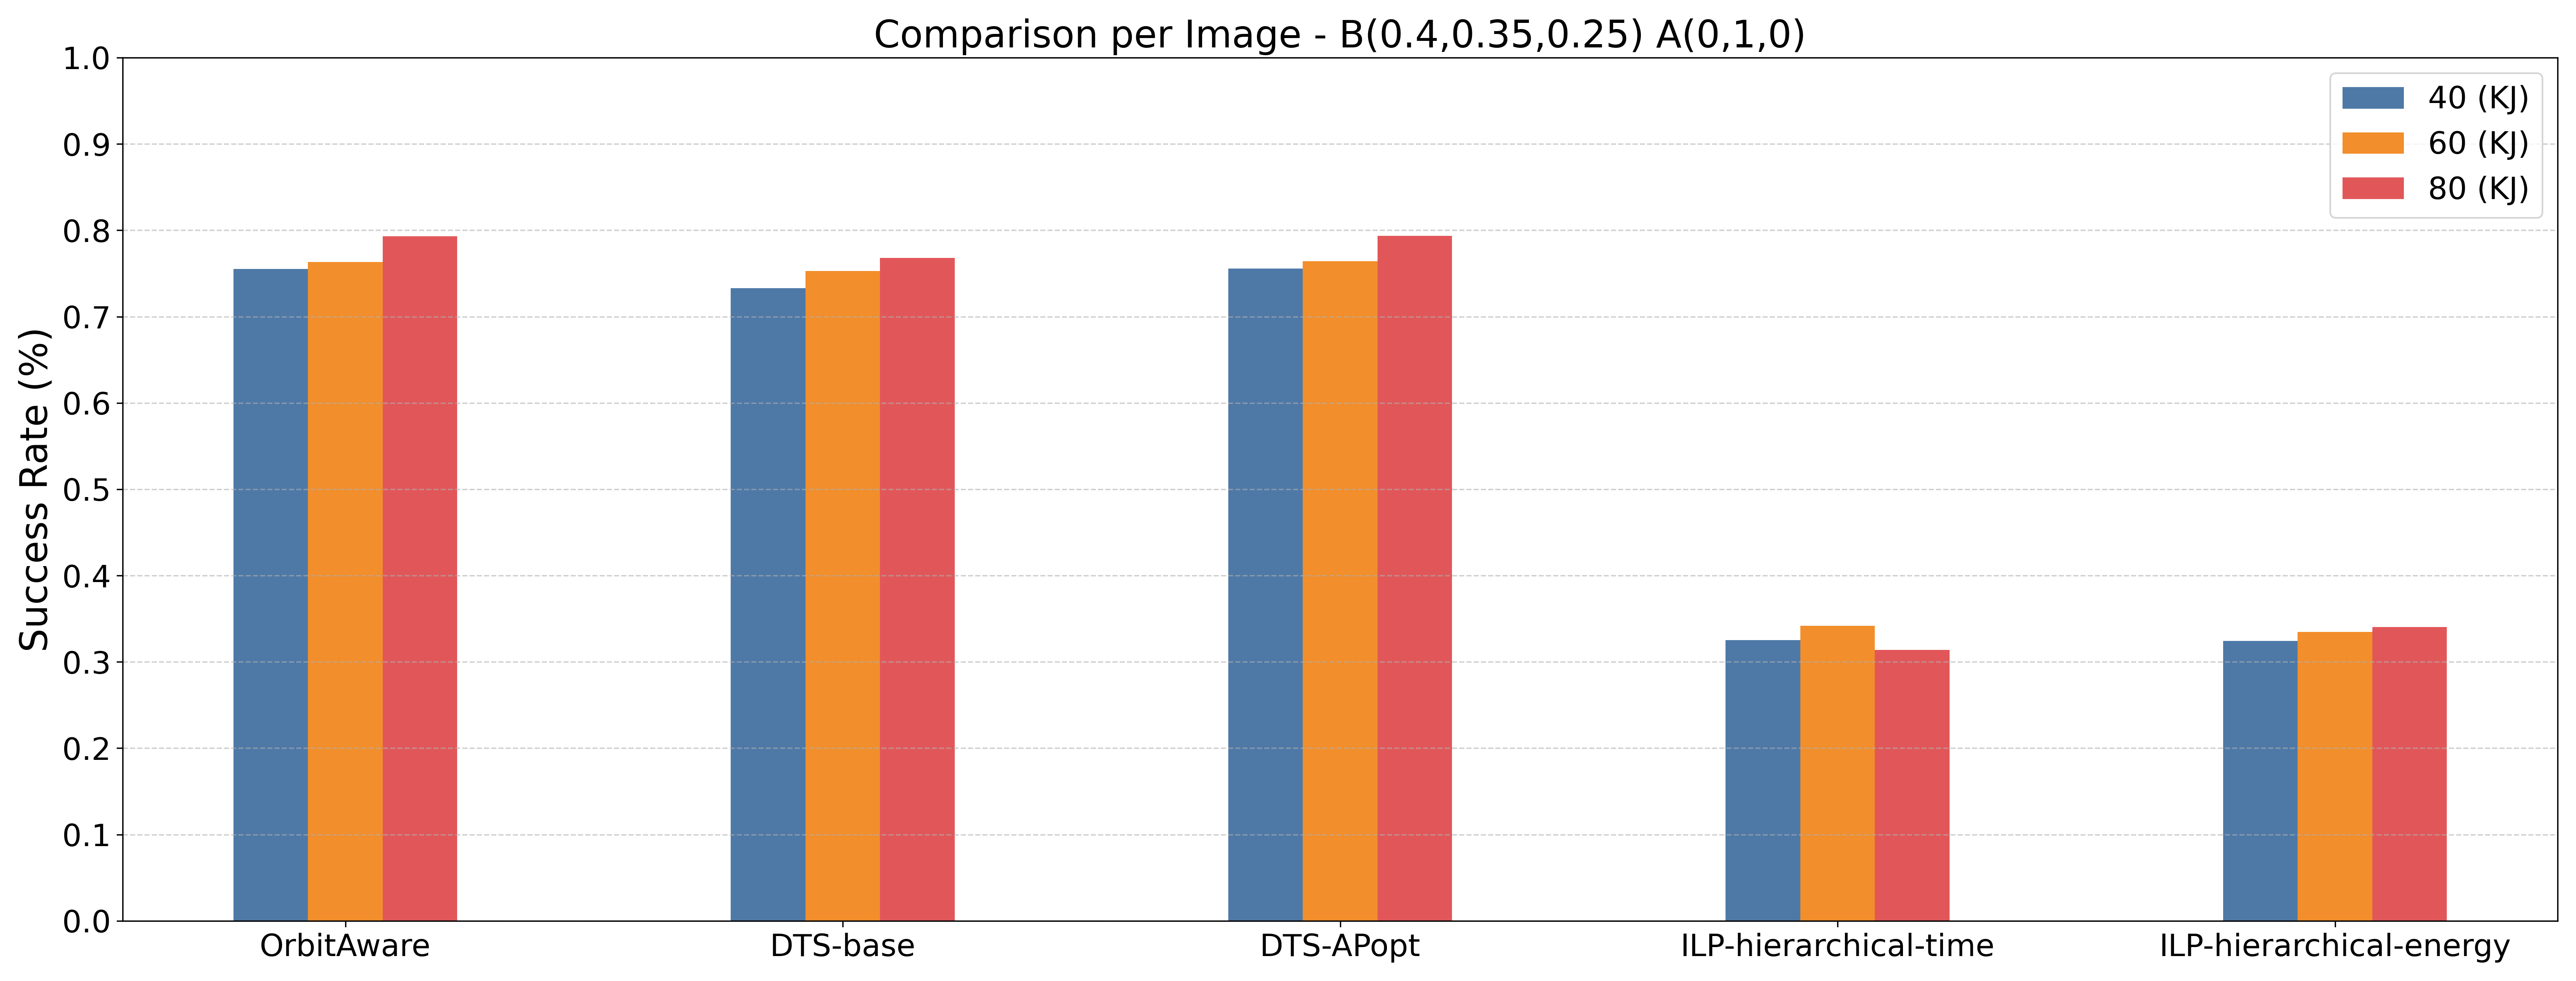
\includegraphics[width=0.9\paperwidth, height=0.4\textheight, keepaspectratio]{comparison_algos_img_0.45_0.35_0.25_0_1_0.png} 
    \caption{Confronto algoritmi con B(0.4,0.35,0.25) A(0,1,0)}
    \label{fig:grafico2}
\end{figure}




\begin{figure}[H] % Forza la posizione 'qui'
    \noindent 
    % --- PRIMO GRAFICO ---
    \hspace*{-3cm} 
    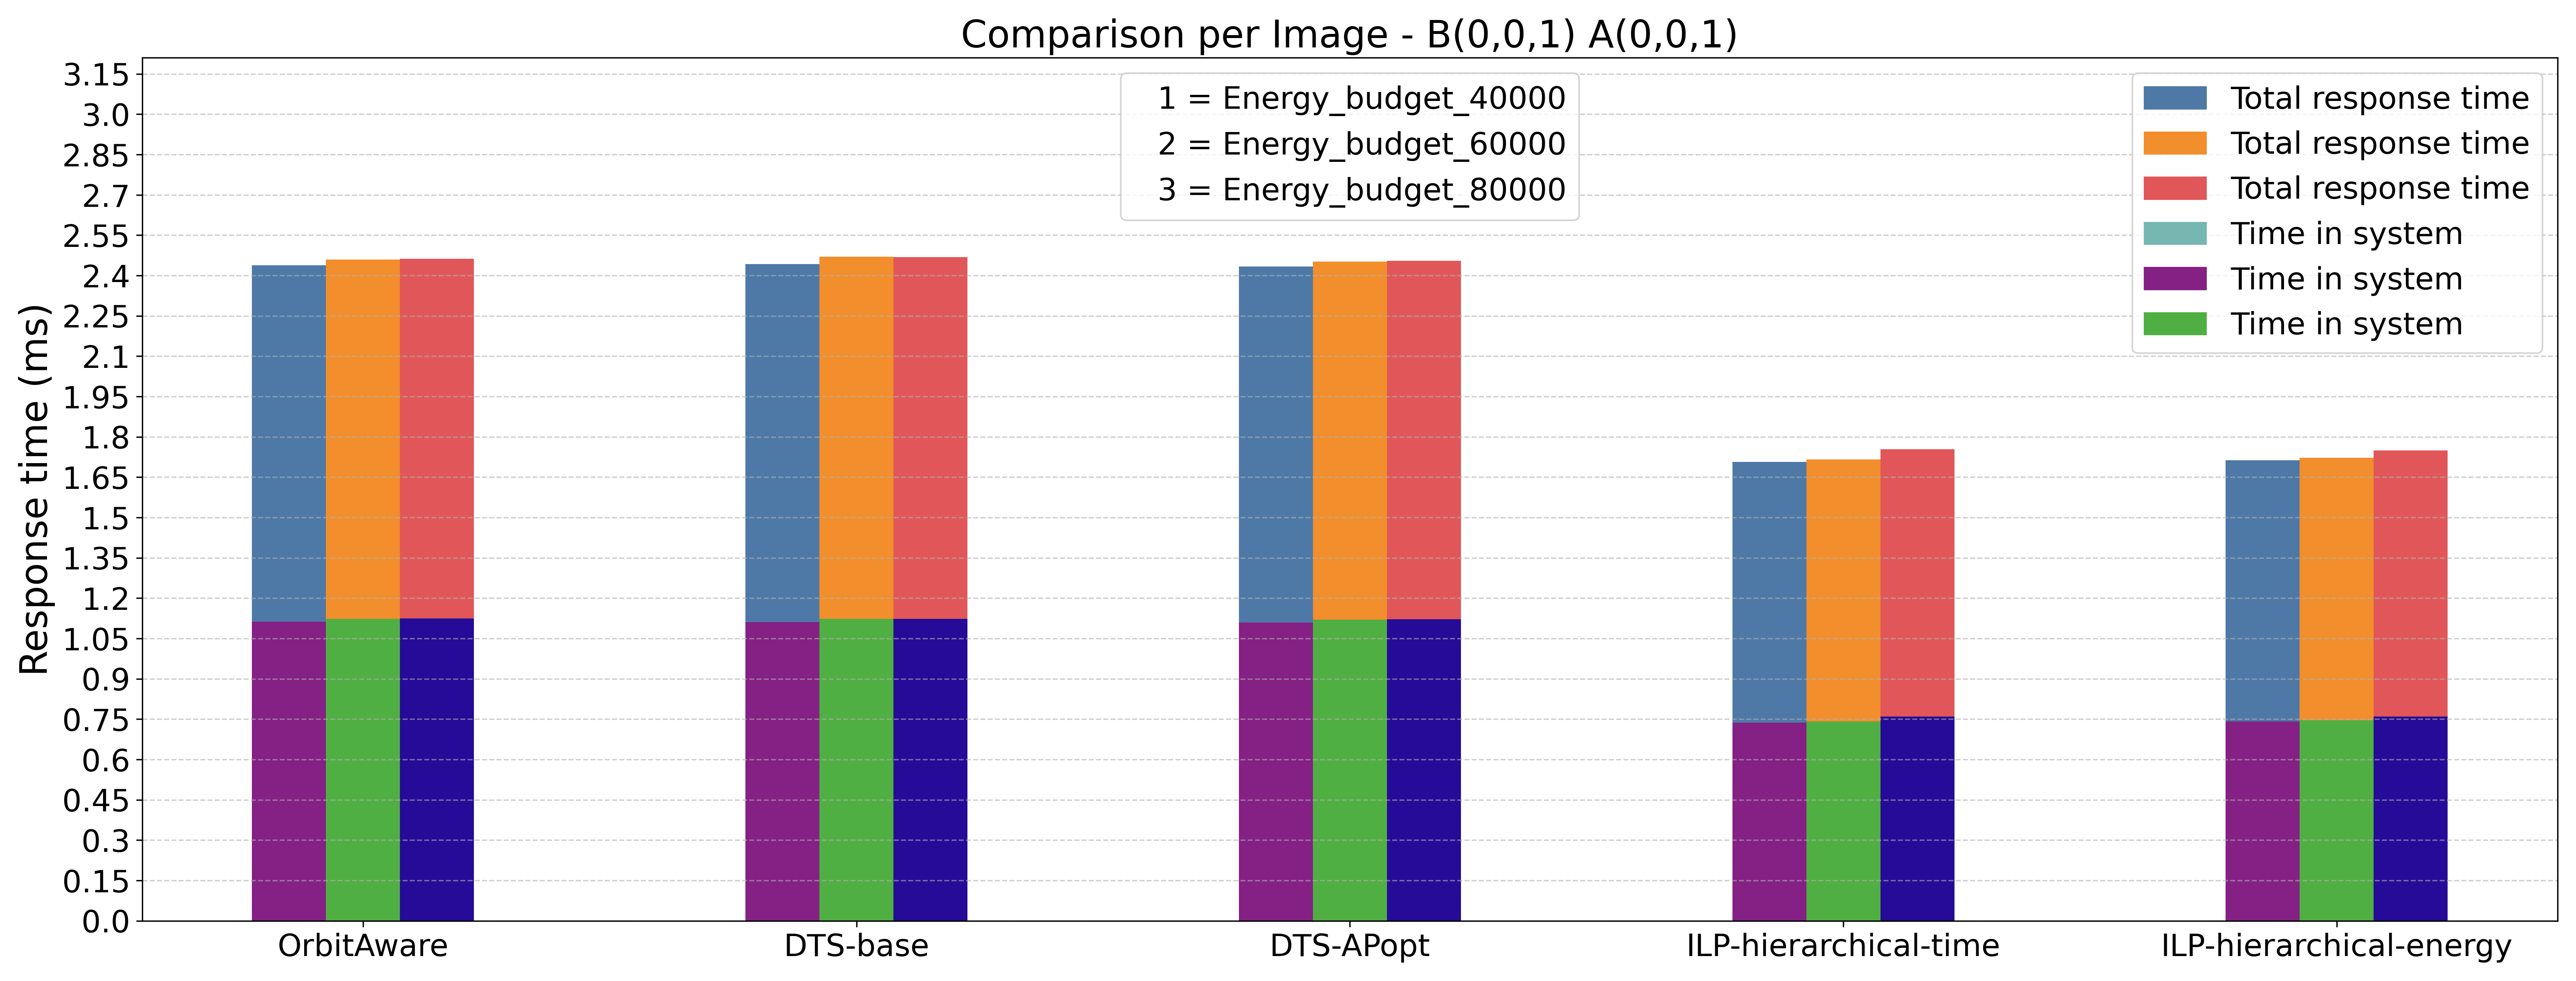
\includegraphics[width=0.9\paperwidth, height=0.4\textheight, keepaspectratio]{B0_0_1A0_0_1.png} 
    \caption{Confronto efficenzza con B(0,0,1) A(0,0,1)}
    \label{fig:grafico1}

    \vspace{1cm} % Spazio verticale tra i due grafici (regolalo a piacere)

    % --- SECONDO GRAFICO ---
    \noindent
    \hspace*{-3cm} 
    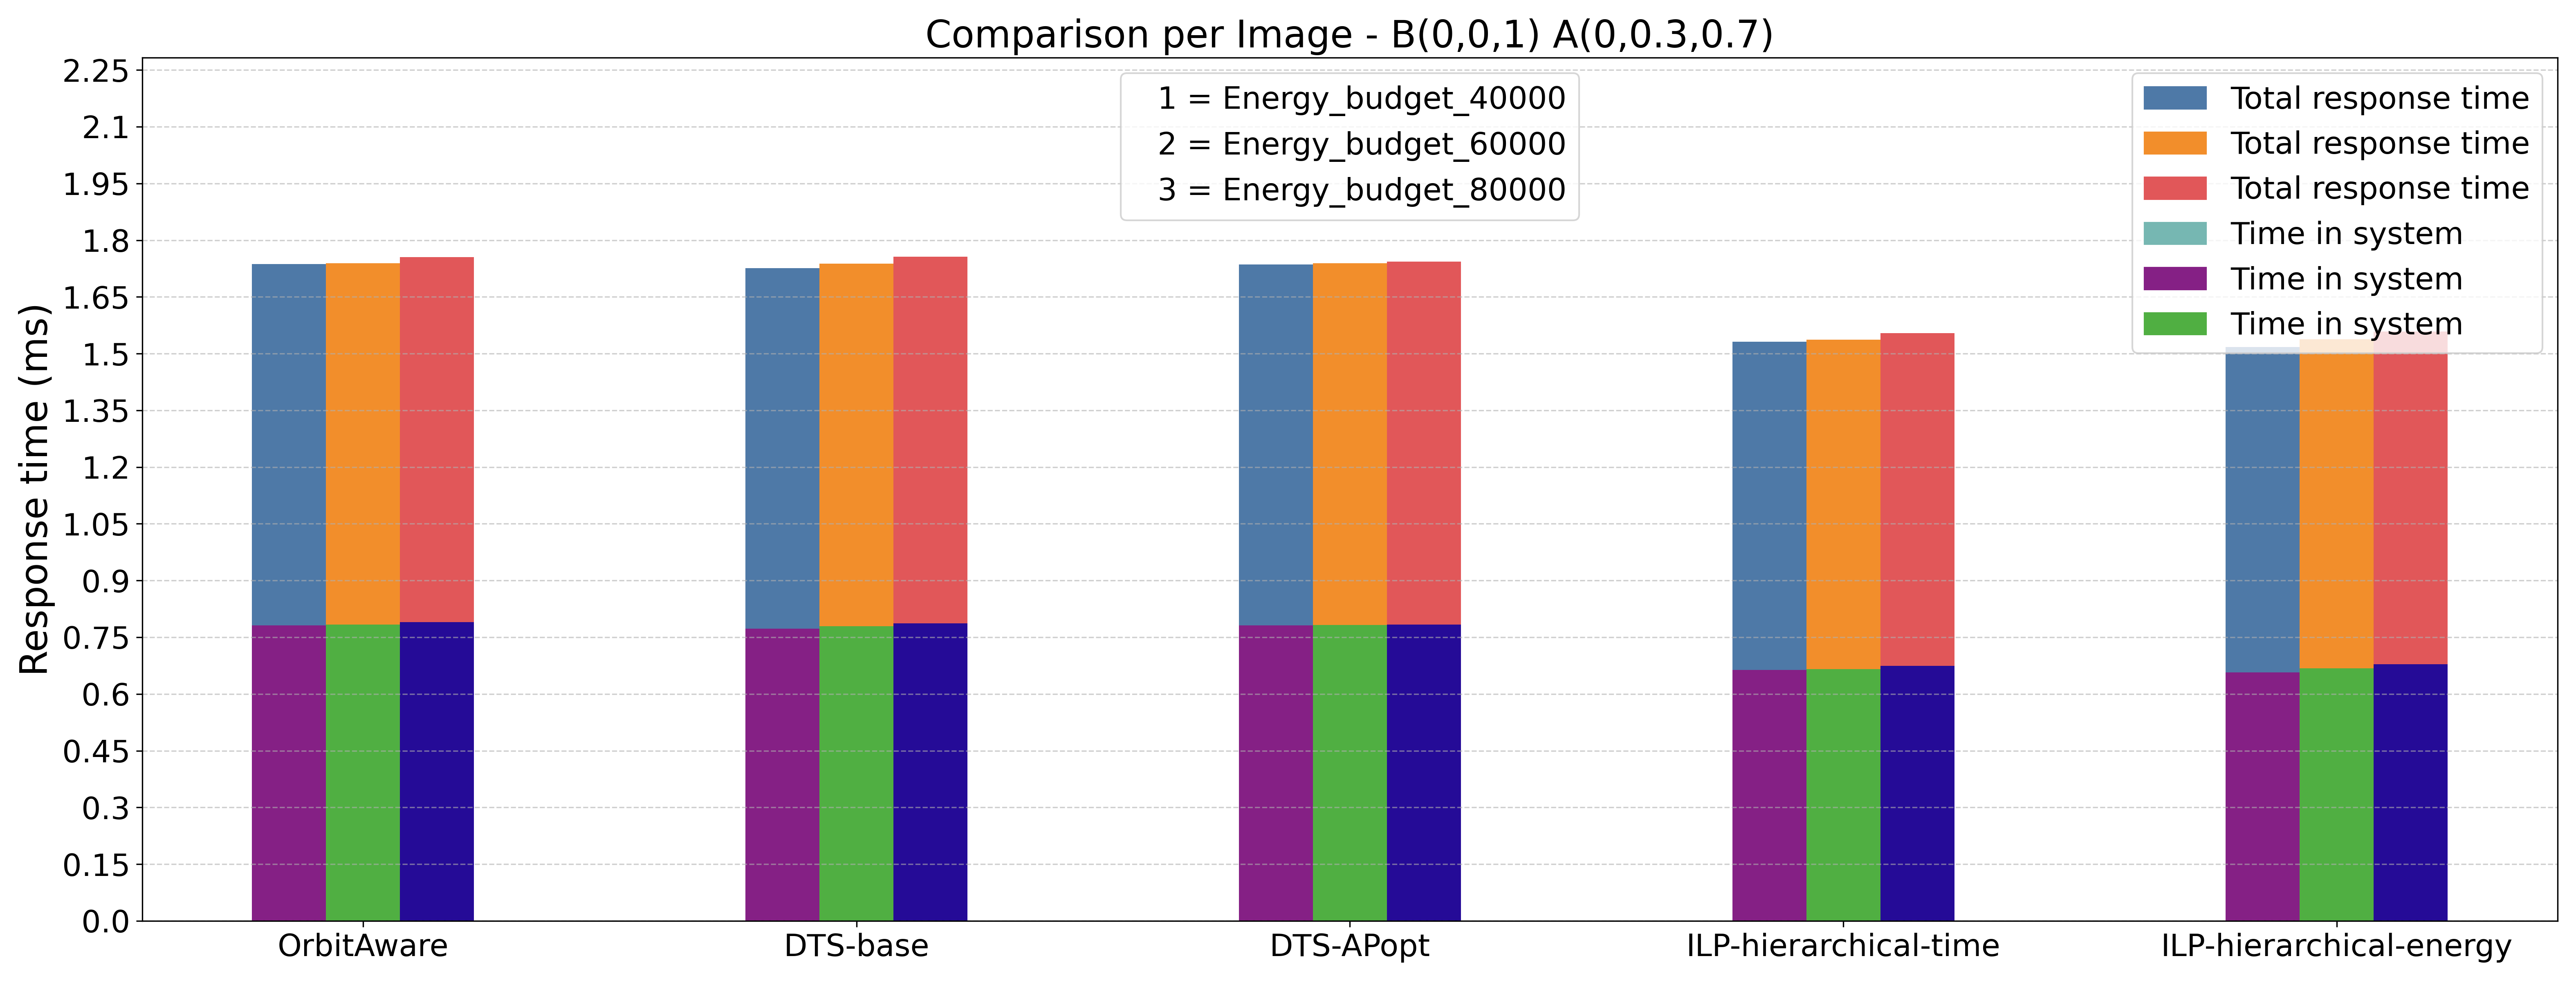
\includegraphics[width=0.9\paperwidth, height=0.4\textheight, keepaspectratio]{B0_0_1A0_0.3_0.7.png} 
    \caption{Confronto efficenza con B(0,0,1) A(0,0.3,0.7)}
    \label{fig:grafico2}
\end{figure}

\begin{figure}[H] % Forza la posizione 'qui'
    \noindent 
    % --- PRIMO GRAFICO ---
    \hspace*{-3cm} 
    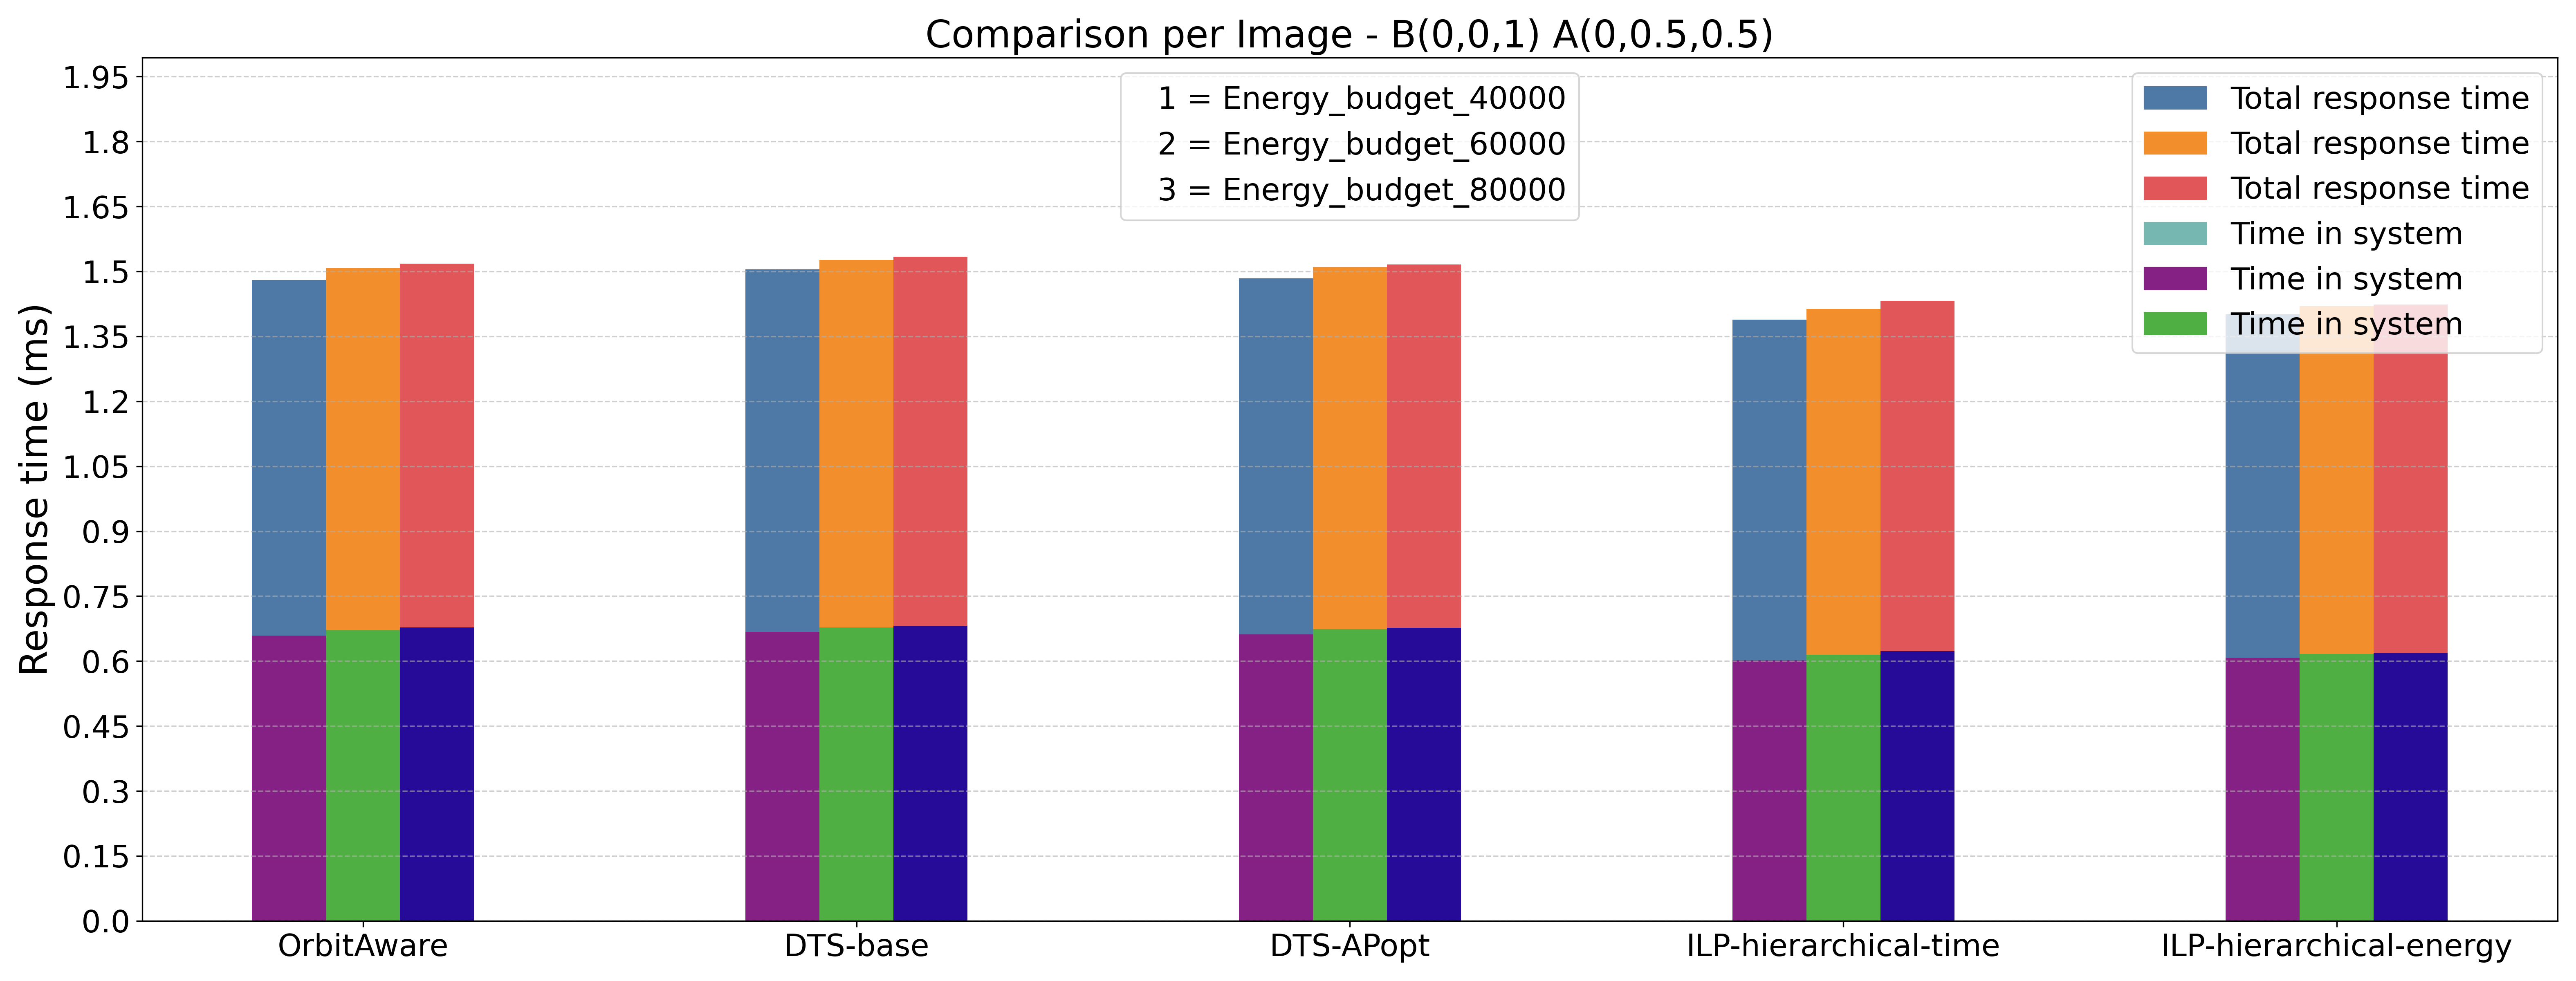
\includegraphics[width=0.9\paperwidth, height=0.4\textheight, keepaspectratio]{B0_0_1A0_0.5_0.5.png} 
    \caption{Confronto efficenza con B(0,0,1) A(0,0.5,0.5)}
    \label{fig:grafico1}

    \vspace{1cm} % Spazio verticale tra i due grafici (regolalo a piacere)

    % --- SECONDO GRAFICO ---
    \noindent
    \hspace*{-3cm} 
    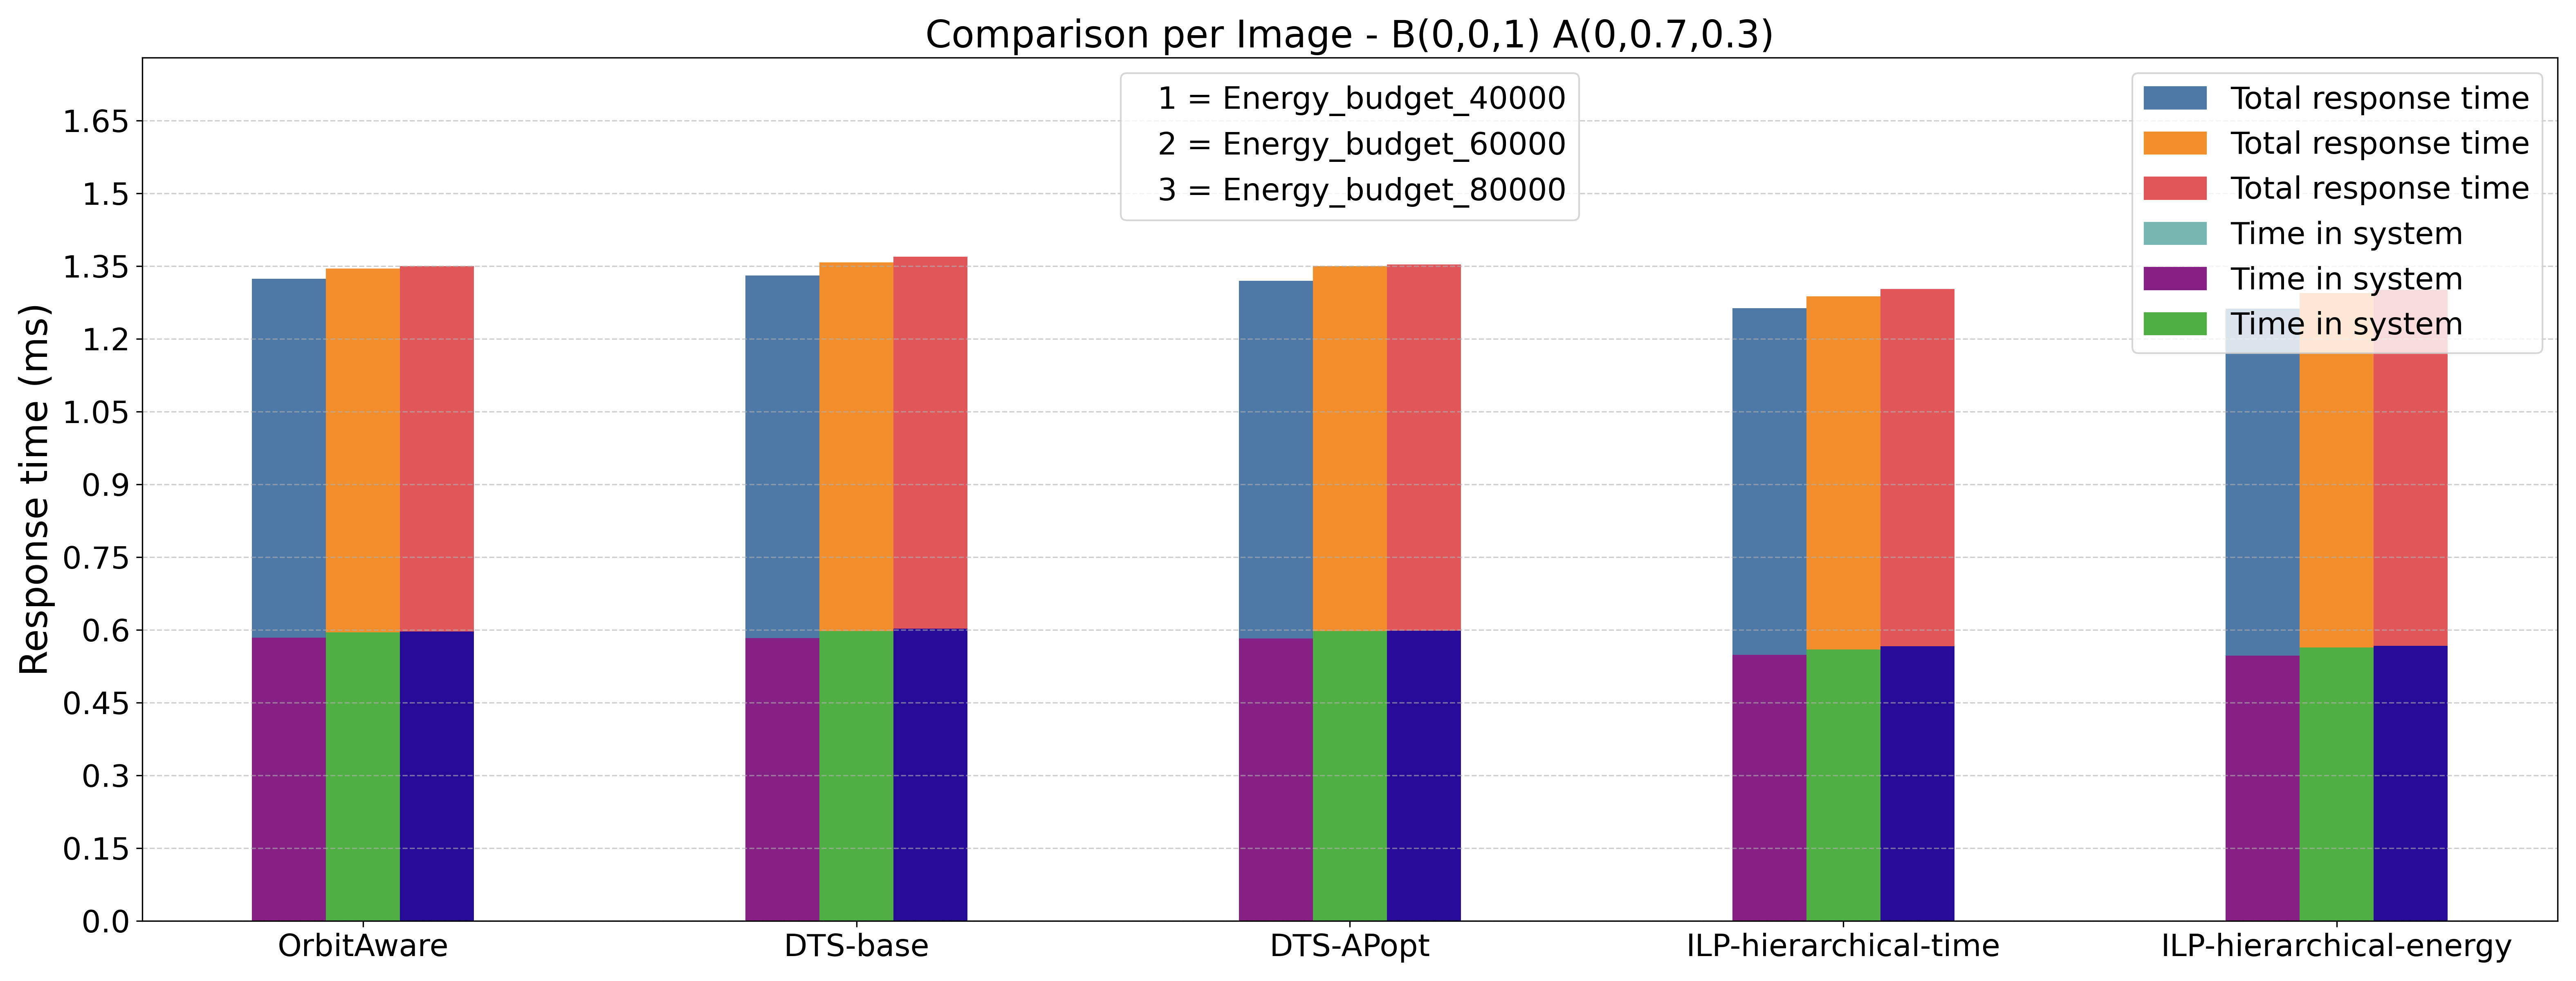
\includegraphics[width=0.9\paperwidth, height=0.4\textheight, keepaspectratio]{B0_0_1A0_0.7_0.3.png} 
    \caption{Confronto efficenza con B(0,0,1) A(0,0.7,0.3)}
    \label{fig:grafico2}
\end{figure}

\begin{figure}[H] % Forza la posizione 'qui'
    \noindent 
    % --- PRIMO GRAFICO ---
    \hspace*{-3cm} 
    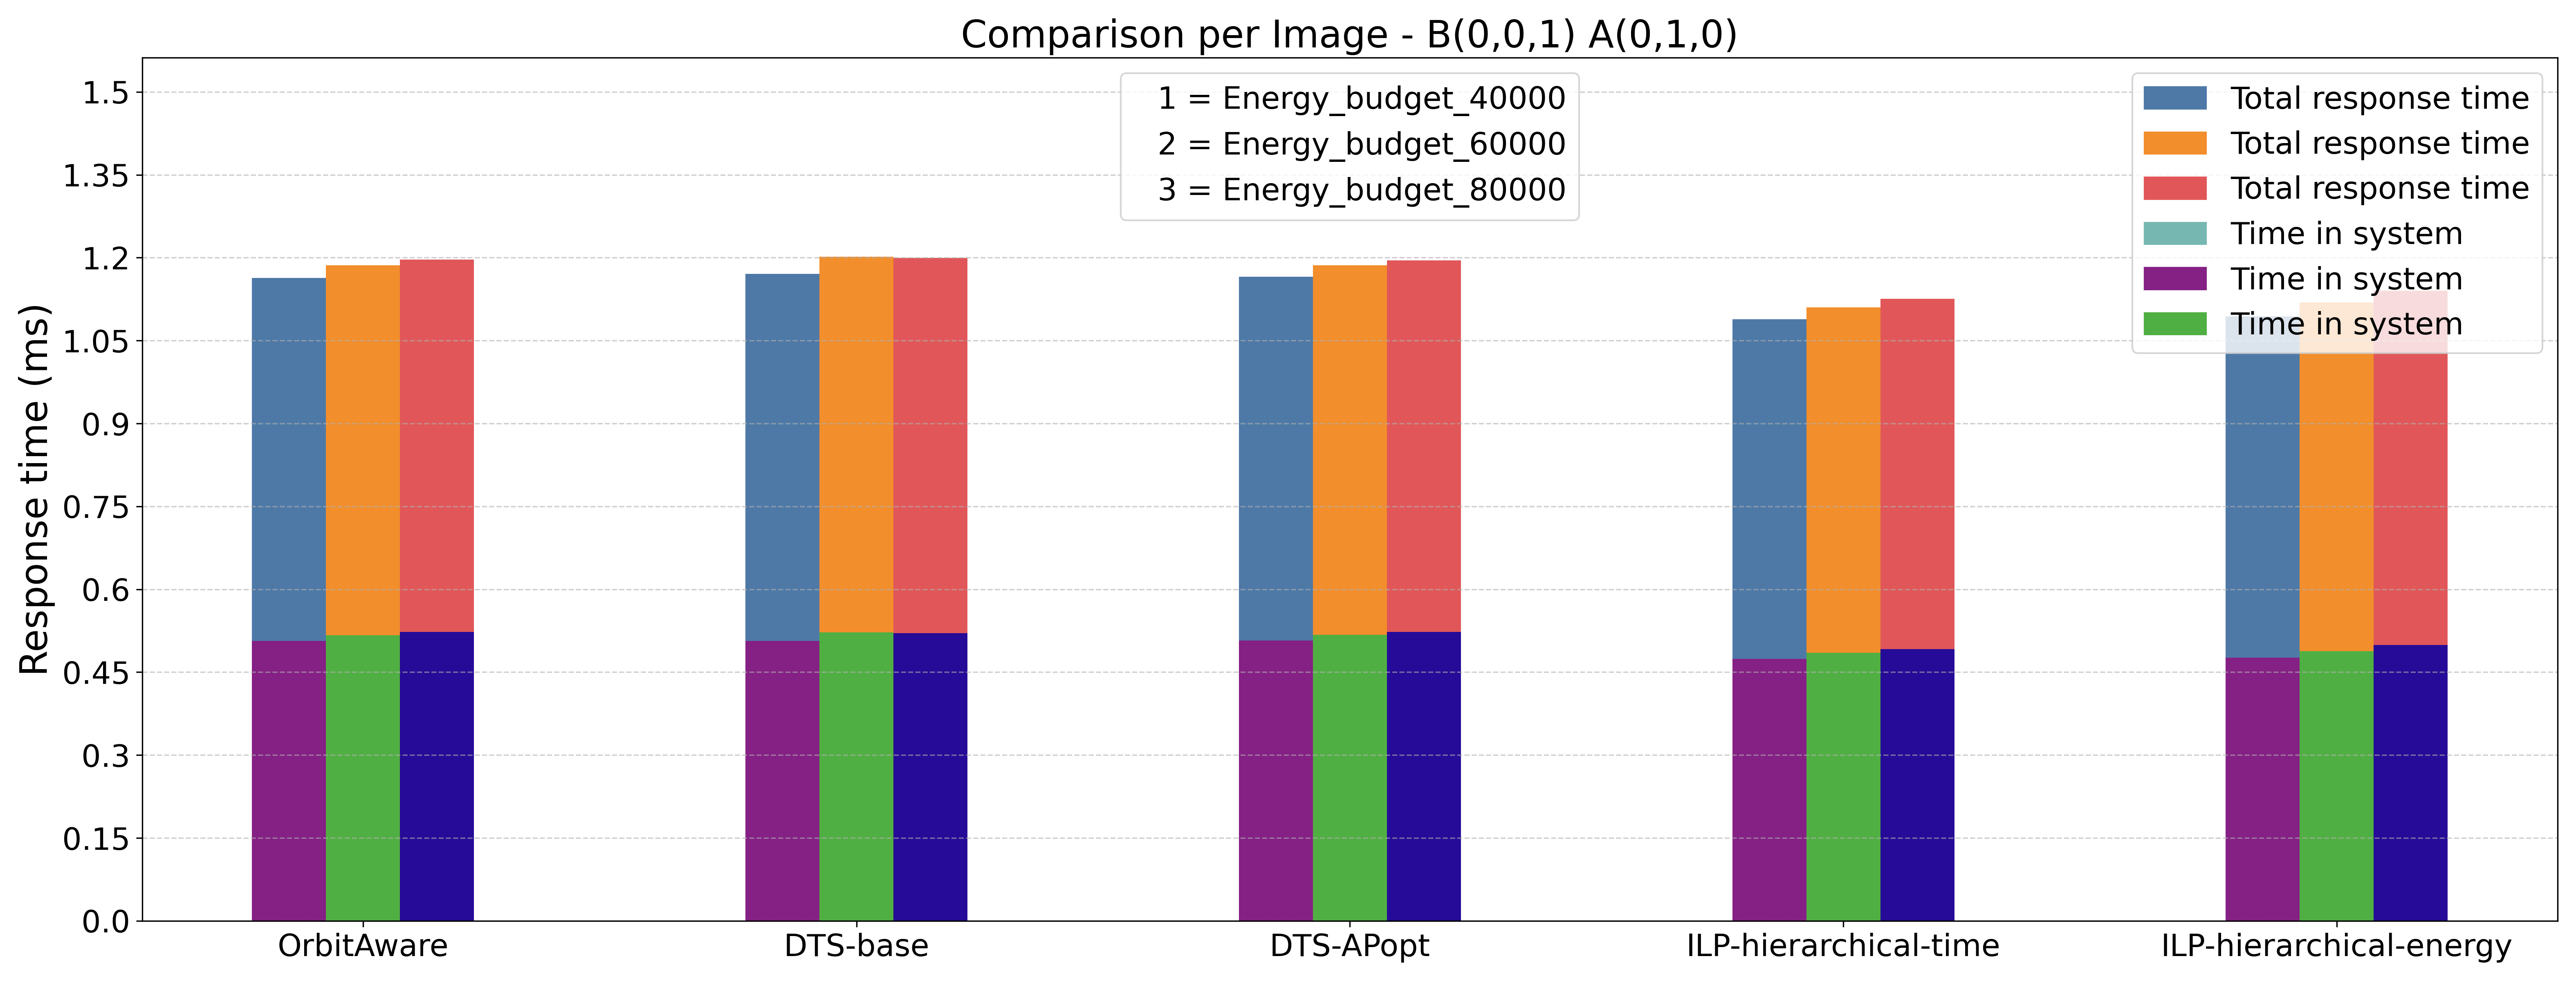
\includegraphics[width=0.9\paperwidth, height=0.4\textheight, keepaspectratio]{B0_0_1A0_1_0.png} 
    \caption{Confronto efficenza con B(0,0,1) A(0,1,0)}
    \label{fig:grafico1}

    \vspace{1cm} % Spazio verticale tra i due grafici (regolalo a piacere)

    % --- SECONDO GRAFICO ---
    \noindent
    \hspace*{-3cm} 
    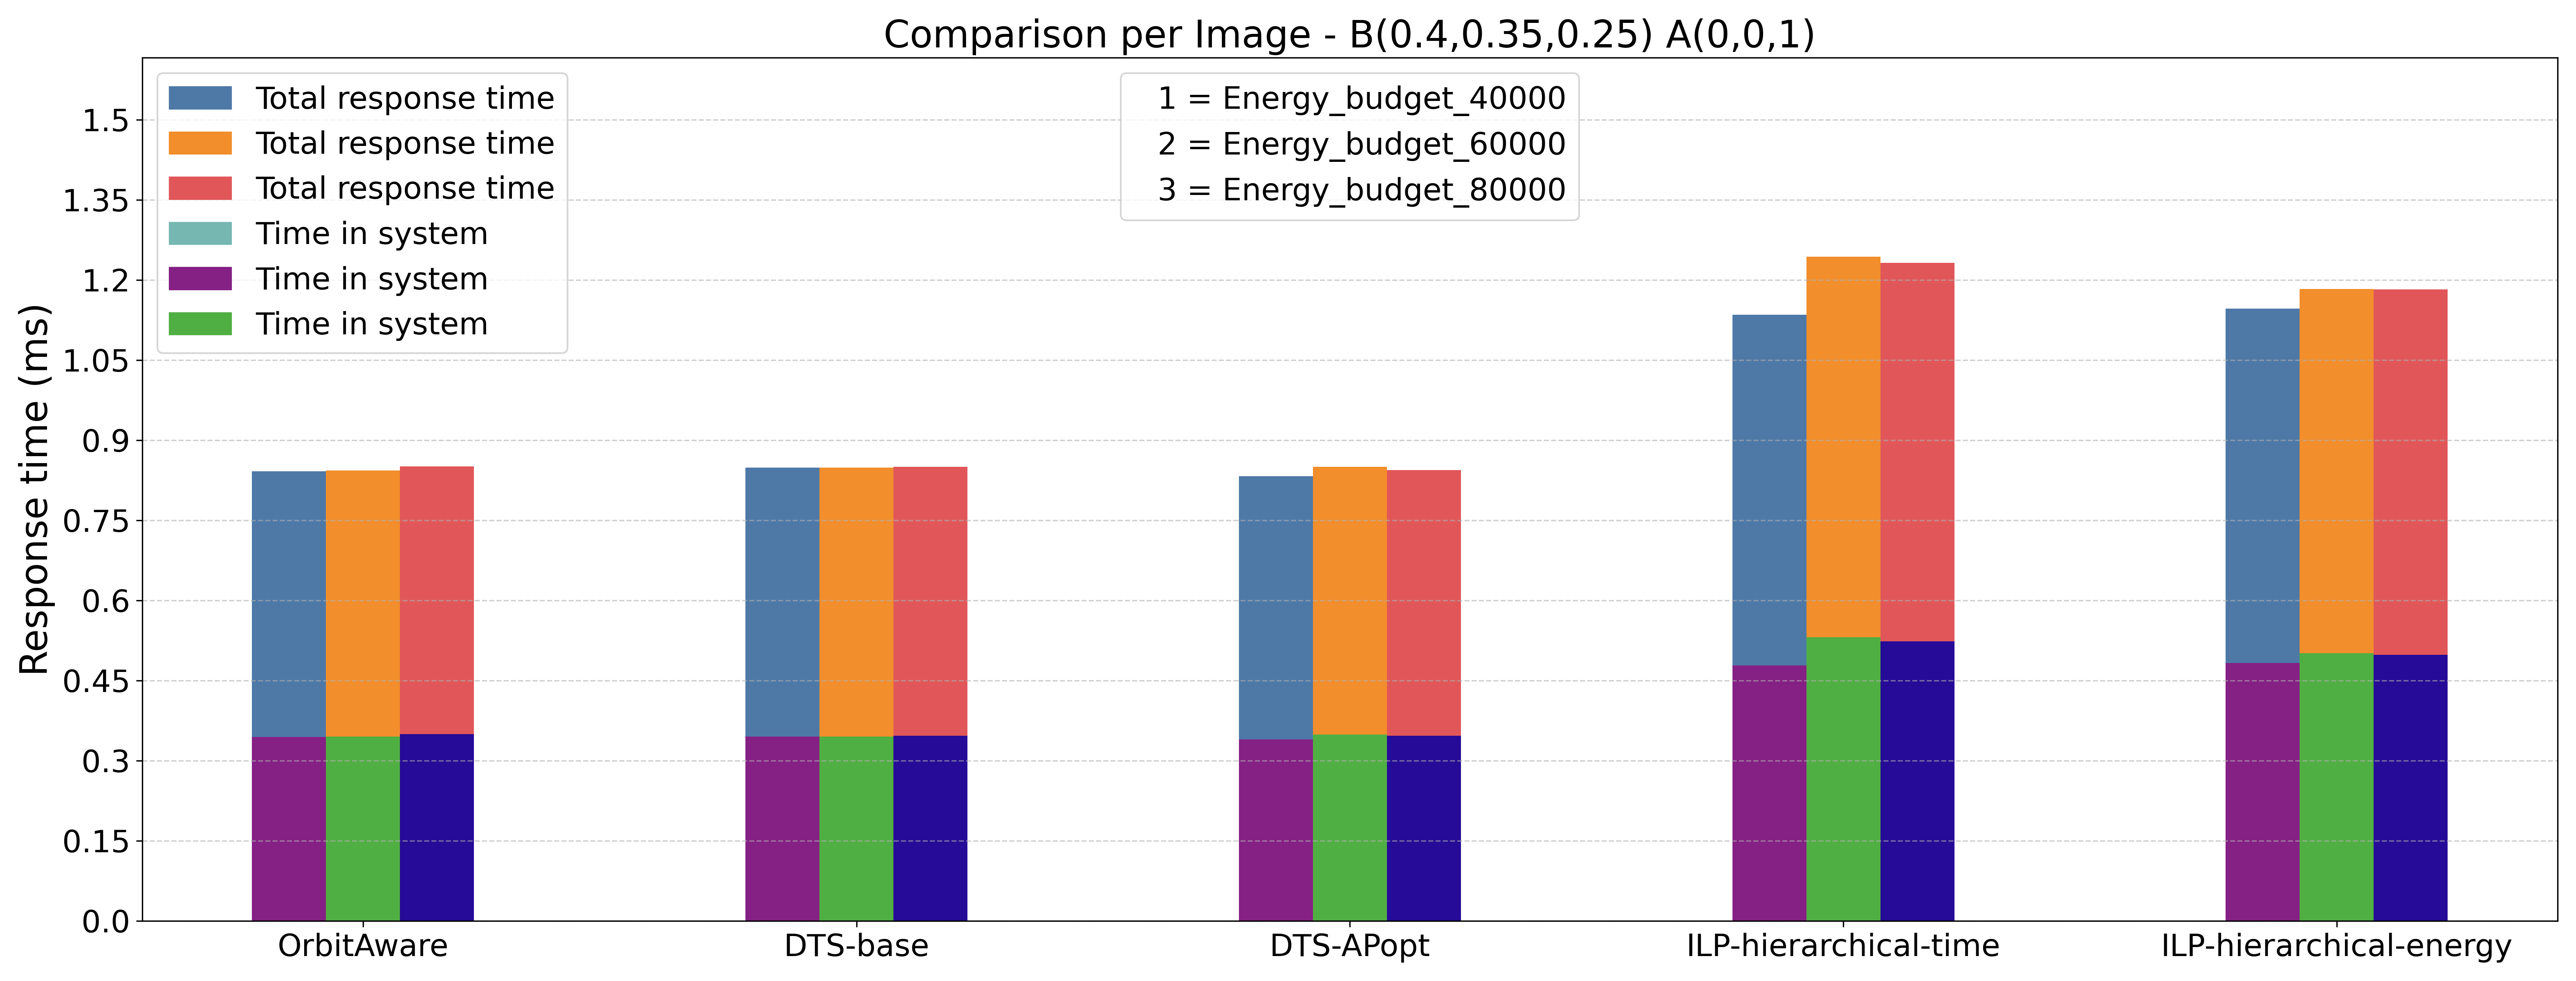
\includegraphics[width=0.9\paperwidth, height=0.4\textheight, keepaspectratio]{B0.4_0.35_0.25A0_0_1.png} 
    \caption{Confronto efficenza con B(0.4,0.35,0.25) A(0,0,1)}
    \label{fig:grafico2}
\end{figure}

\begin{figure}[H] % Forza la posizione 'qui'
    \noindent 
    % --- PRIMO GRAFICO ---
    \hspace*{-3cm} 
    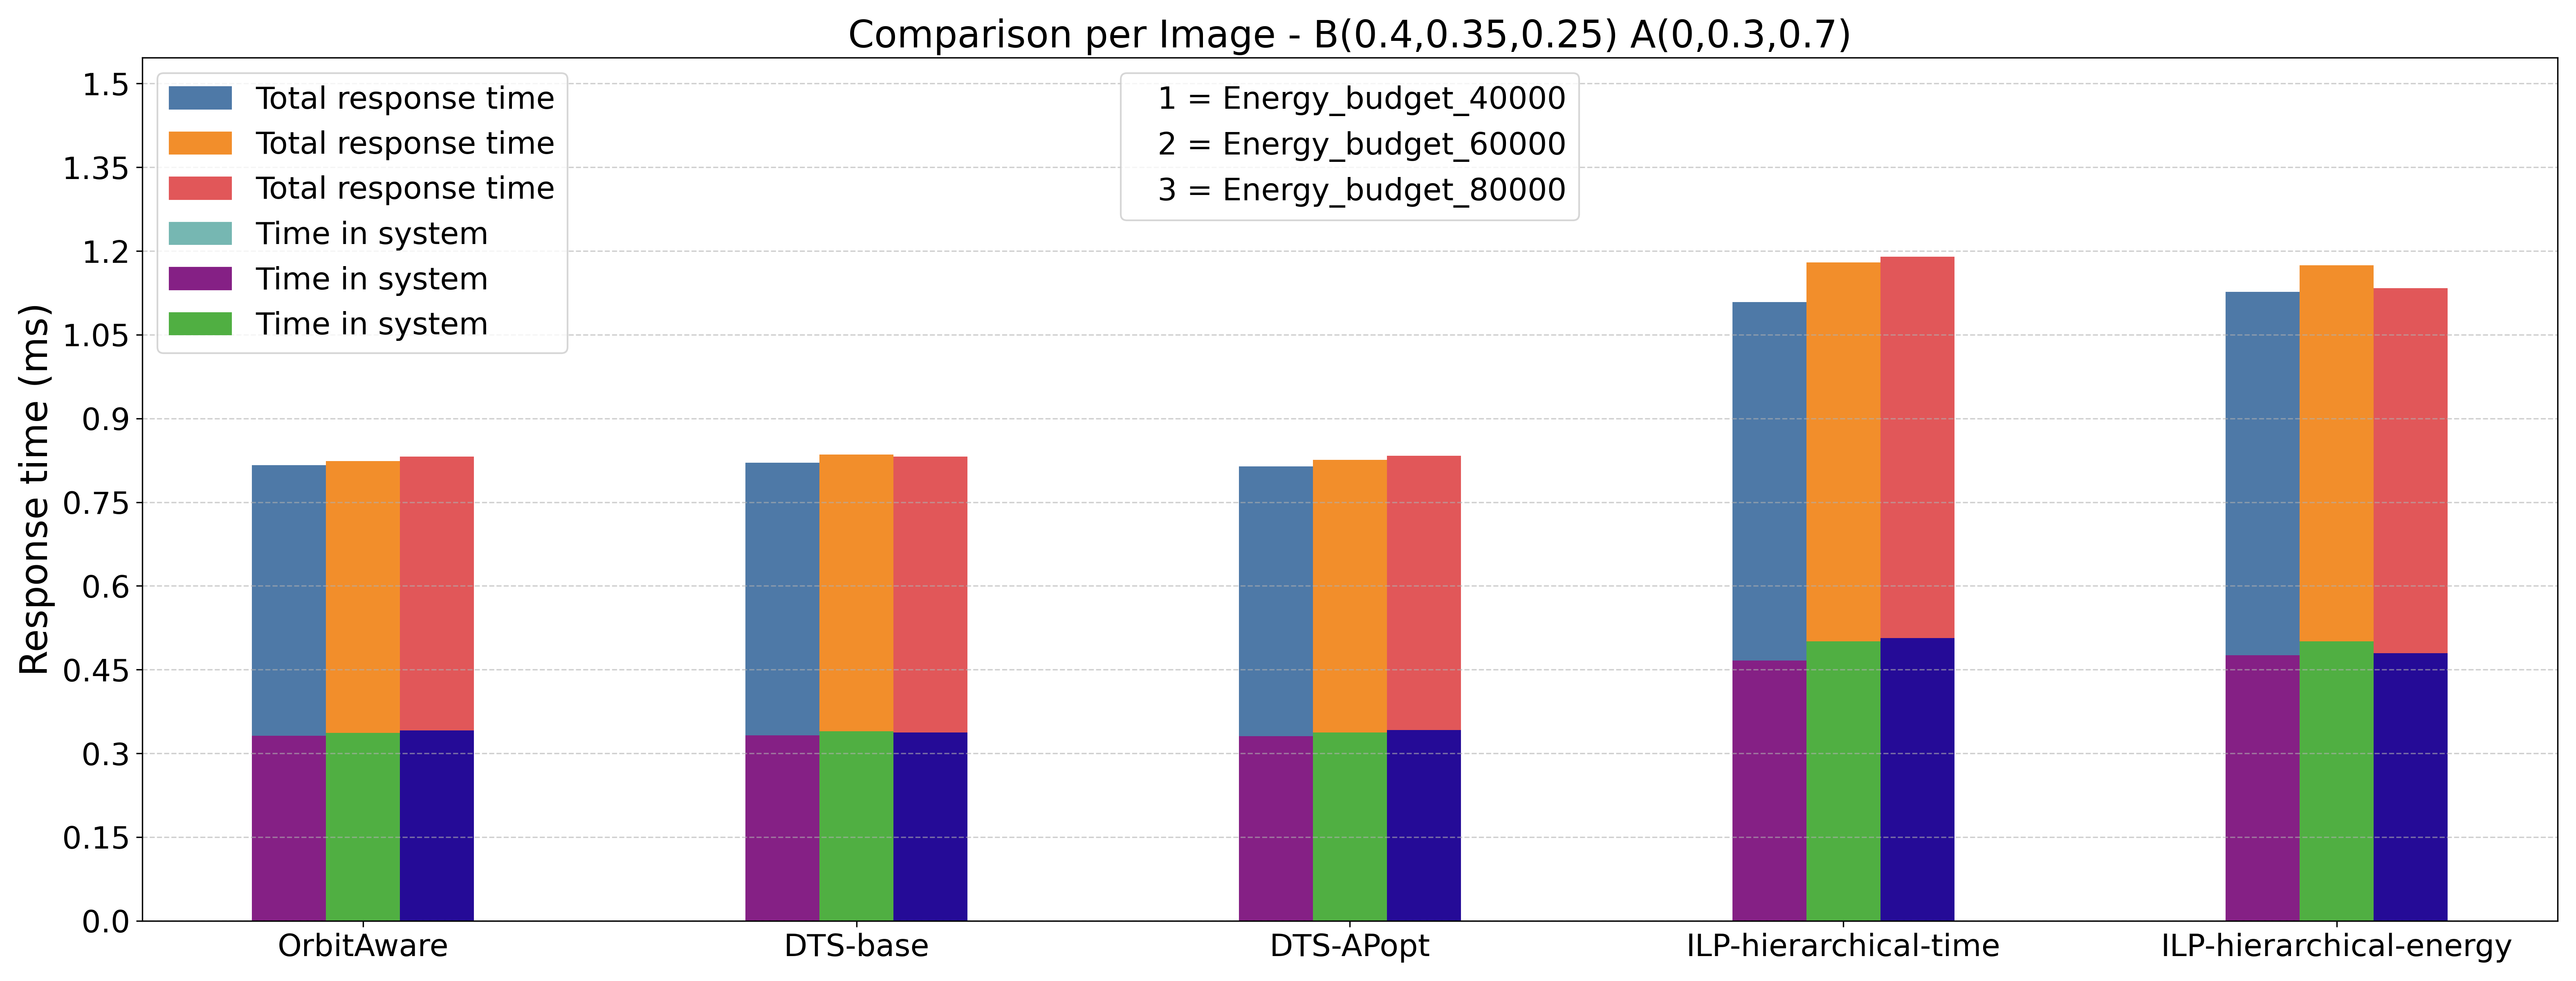
\includegraphics[width=0.9\paperwidth, height=0.4\textheight, keepaspectratio]{B0.4_0.35_0.25A0_0.3_0.7.png} 
    \caption{Confronto efficenza con B(0.4,0.35,0.25) A(0,0.3,0.7)}
    \label{fig:grafico1}

    \vspace{1cm} % Spazio verticale tra i due grafici (regolalo a piacere)

    % --- SECONDO GRAFICO ---
    \noindent
    \hspace*{-3cm} 
    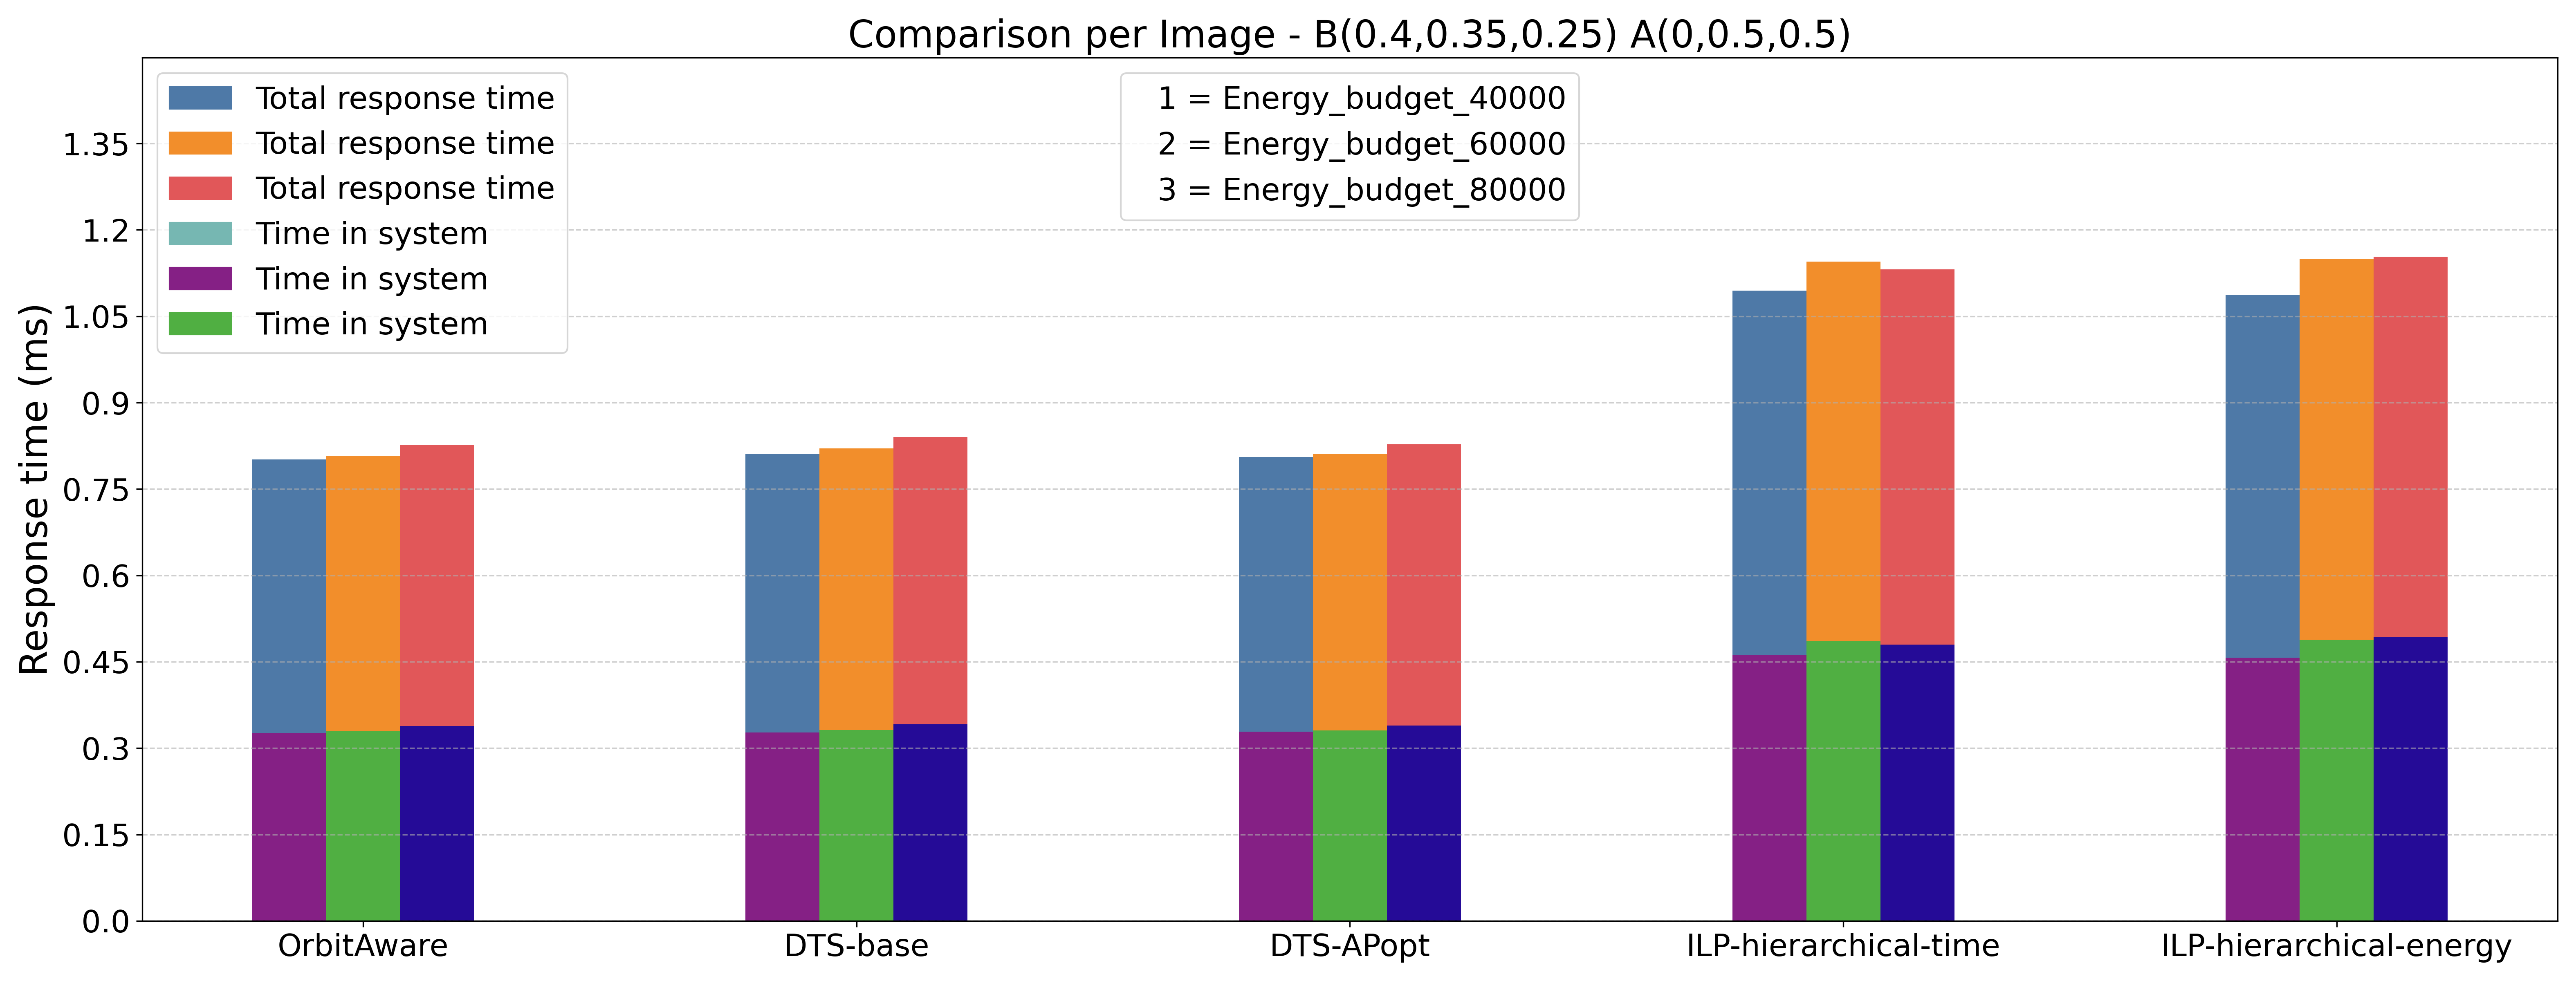
\includegraphics[width=0.9\paperwidth, height=0.4\textheight, keepaspectratio]{B0.4_0.35_0.25A0_0.5_0.5.png} 
    \caption{Confronto efficenza con B(0.4,0.35,0.25) A(0,0.5,0.5)}
    \label{fig:grafico2}
\end{figure}

\begin{figure}[H] % Forza la posizione 'qui'
    \noindent 
    % --- PRIMO GRAFICO ---
    \hspace*{-3cm} 
    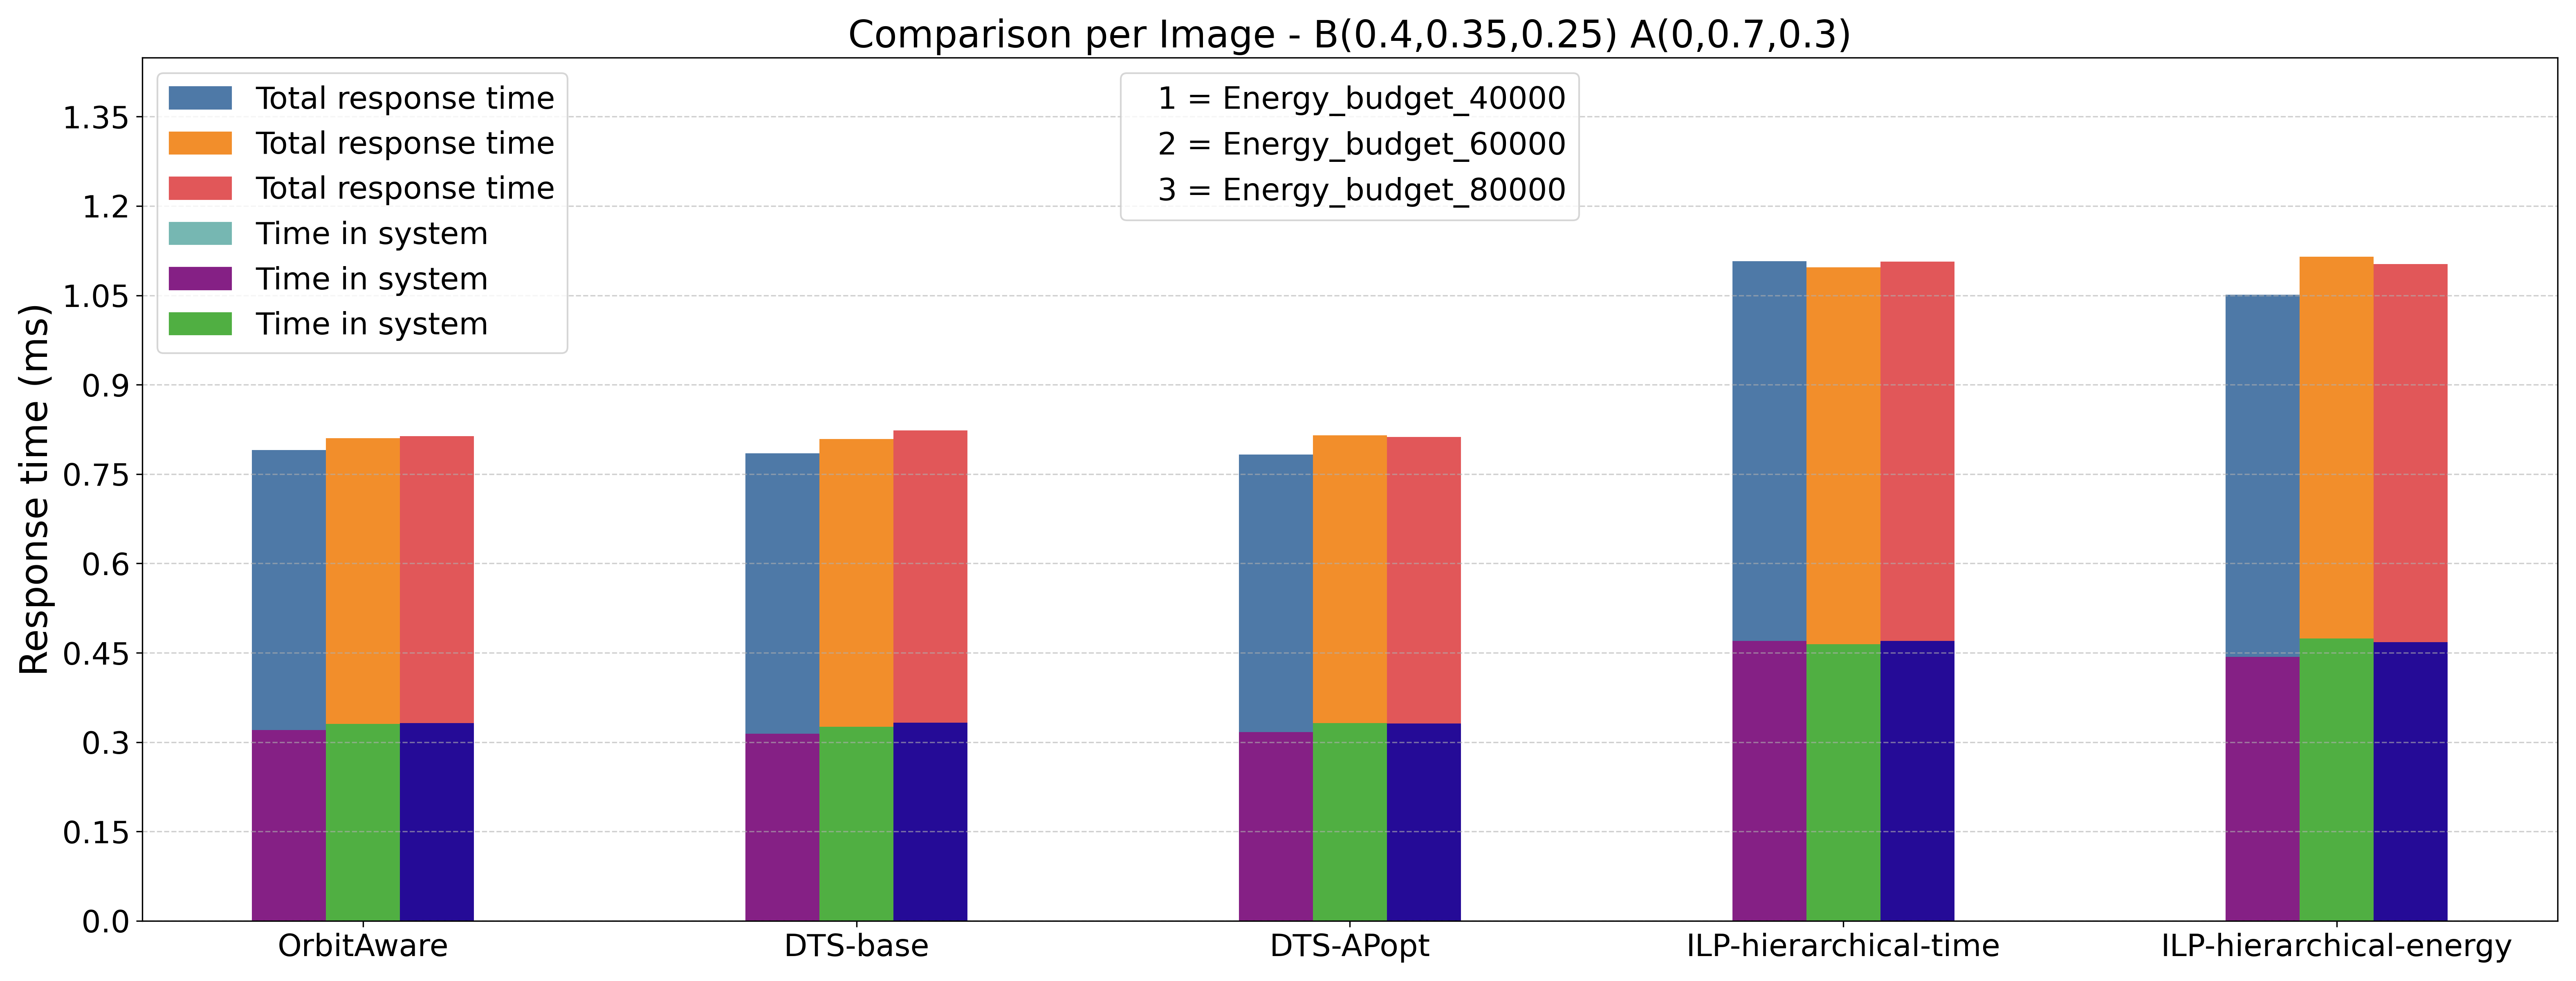
\includegraphics[width=0.9\paperwidth, height=0.4\textheight, keepaspectratio]{B0.4_0.35_0.25A0_0.7_0.3.png} 
    \caption{Confronto efficenza con B(0.4,0.35,0.25) A(0,0.7,0.3)}
    \label{fig:grafico1}

    \vspace{1cm} % Spazio verticale tra i due grafici (regolalo a piacere)

    % --- SECONDO GRAFICO ---
    \noindent
    \hspace*{-3cm} 
    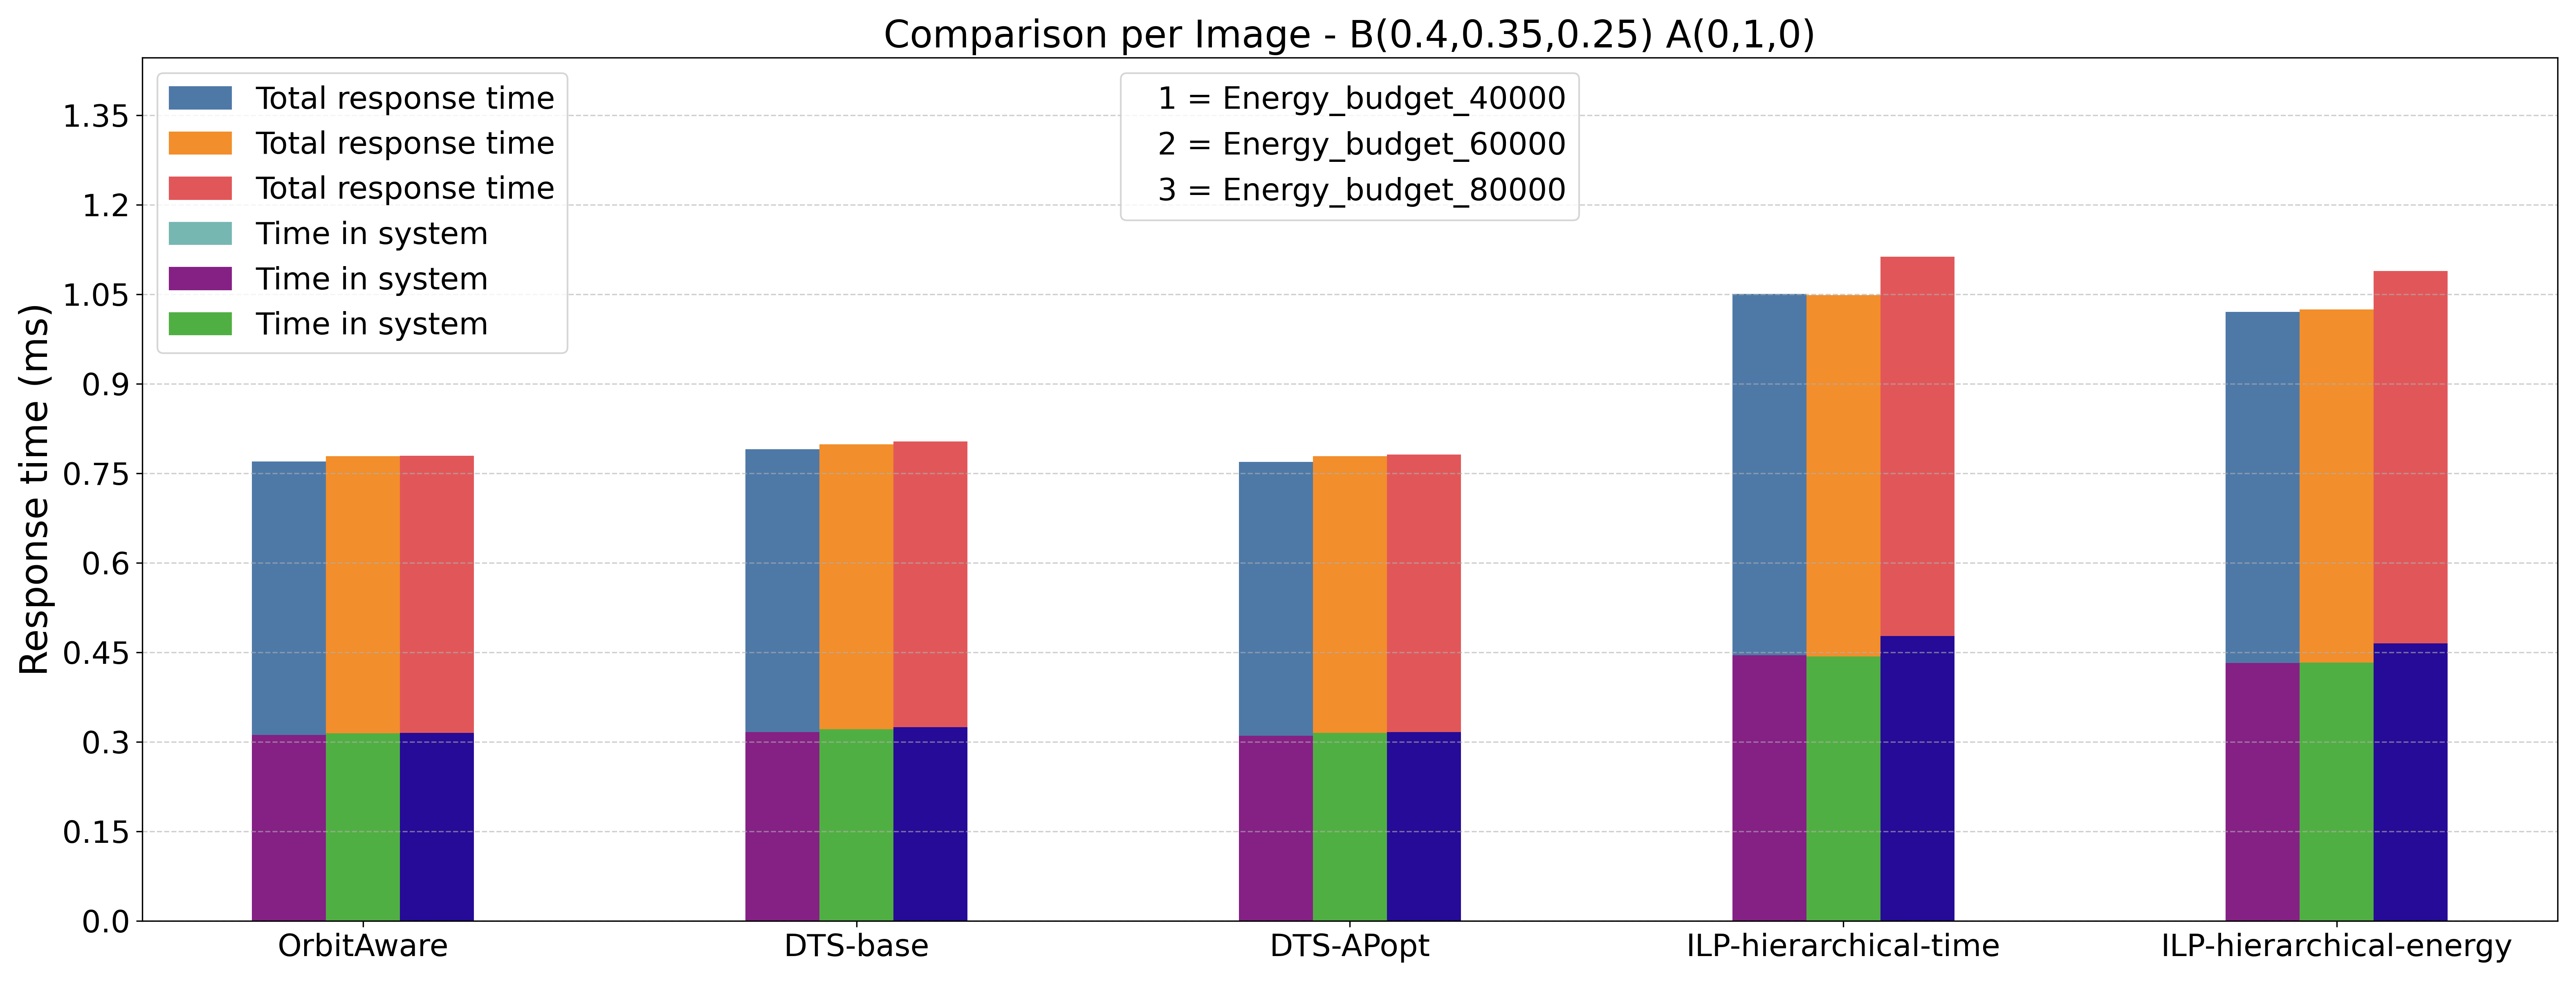
\includegraphics[width=0.9\paperwidth, height=0.4\textheight, keepaspectratio]{B0.4_0.35_0.25A0_1_0.png} 
    \caption{Confronto efficenza con B(0.4,0.35,0.25) A(0,1,0)}
    \label{fig:grafico2}
\end{figure}

\end{document}